\documentclass{cmspaper}
\usepackage{graphicx}
\usepackage{amsmath}
\usepackage{amssymb}
\usepackage{subfigure}
\usepackage{multirow}
\usepackage[pdfborder=0 0 0,
            colorlinks,
            urlcolor = blue,
            linkcolor = black,
            citecolor = black,
            menucolor = black,]
           {hyperref}
%% \usepackage[colorlinks]{hyperref}
%% \usepackage{url}
\usepackage[toc,page]{appendix}
\usepackage{varioref}
\renewcommand{\appendixname}{Appendix}
%% \renewcommand{\appendixtocname}{List of appendices}

% \input{privsym}
\newcommand{\CLs}{\ensuremath{CL_\mathrm{s}}}
\newcommand{\CLb}{\ensuremath{CL_\mathrm{b}}}
\newcommand{\CLsb}{\ensuremath{CL_\mathrm{s+b}}}

\newcommand{\GeV}{\ensuremath{\mathrm{Ge\kern -0.1em V}}}
\newcommand{\TeV}{\ensuremath{\mathrm{Te\kern -0.1em V}}}
\newcommand{\TeVcc}{\ensuremath{\,\mathrm{Te\kern -0.1em V\!/c}^2}}
\newcommand{\GeVcc}{\ensuremath{\,\mathrm{Ge\kern -0.1em V\!/c}^2}}
\newcommand{\MeVcc}{\ensuremath{\,\mathrm{Me\kern -0.1em V\!/c}^2}}
\newcommand{\GeVc}{\ensuremath{\mathrm{Ge\kern -0.1em V}\!/c}}
\newcommand{\nanob}{\mbox{{\rm ~nb}~}}
\newcommand{\fb}{\ensuremath{\mathrm{fb}}}
\newcommand{\pb}{\ensuremath{\mathrm{pb}}}
\newcommand{\ifb}{\ensuremath{\mathrm{fb^{-1}}}}
\newcommand{\ipb}{\ensuremath{\mathrm{pb^{-1}}}}
\newcommand{\grad}{\ensuremath{^{\circ}}}
%
% Special user made math symbols
%
\newcommand{\lsim}{\raisebox{-1.5mm}{$\:\stackrel{\textstyle{<}}{\textstyle{\sim}}\:$}}
\newcommand{\gsim}{\raisebox{-1.5mm}{$\:\stackrel{\textstyle{>}}{\textstyle{\sim}}\:$}}

% particles

\newcommand{\pipm}{\ensuremath{\pi^{\pm}}}
\newcommand{\pizero}{\ensuremath{\pi^{0}}}
\newcommand{\Hi}{\ensuremath{\mathrm{H}}}
\newcommand{\W}{\ensuremath{\mathrm{W}}}
\newcommand{\Wjets}{\ensuremath{\mathrm{W+jets}}}
\newcommand{\Zjets}{\ensuremath{\mathrm{Z+jets}}}
\newcommand{\Wt}{\ensuremath{\mathrm{Wt}}}
\newcommand{\Wstar}{\ensuremath{\mathrm{W}^{*}}}
\newcommand{\Wparenthesisstar}{\ensuremath{\mathrm{W}^{(*)}}}
\newcommand{\WW}{\ensuremath{\W^+\W^-}}
\newcommand{\Z}{\ensuremath{\mathrm{Z}}}
\newcommand{\Zstar}{\ensuremath{\mathrm{Z}^{*}}}
\newcommand{\Astar}{\ensuremath{\mathrm{\gamma}^{*}}}
\newcommand{\ZZ}{\ensuremath{\Z\Z}}
\newcommand{\WZ}{\ensuremath{\W\Z}}
\newcommand{\Wgstar}{\ensuremath{\W\Astar}}
\newcommand{\E}{\ensuremath{\mathrm{e}}}
\newcommand{\Ep}{\ensuremath{\mathrm{e}^{+}}}
\newcommand{\Em}{\ensuremath{\mathrm{e}^{-}}}
\newcommand{\Epm}{\ensuremath{\mathrm{e}^{\pm}}}
\newcommand{\Emp}{\ensuremath{\mathrm{e}^{\mp}}}
\newcommand{\M}{\ensuremath{\mu}}
\newcommand{\Mp}{\ensuremath{\mu^{+}}}
\newcommand{\Mm}{\ensuremath{\mu^{-}}}
\newcommand{\Mpm}{\ensuremath{\mu^{\pm}}}
\newcommand{\Mmp}{\ensuremath{\mu^{\mp}}}
\newcommand{\Tau}{\ensuremath{\tau}}
\newcommand{\Nu}{\ensuremath{\nu}}
\newcommand{\Nubar}{\ensuremath{\bar{\nu}}}
\newcommand{\Lep}{\ensuremath{\ell}}
\newcommand{\Lepp}{\ensuremath{\ell^{+}}}
\newcommand{\Lepm}{\ensuremath{\ell^{-}}}
\newcommand{\Lprime}{\ensuremath{\Lep^{\prime}}}
\newcommand{\Prot}{\ensuremath{\mathrm{p}}}
\newcommand{\Pbar}{\ensuremath{\bar{\mathrm{p}}}}
\newcommand{\PP}{\Prot\Prot}
\newcommand{\PPbar}{\Prot\Pbar}
\newcommand{\ttbar}{\ensuremath{\mathrm{t}\bar{\mathrm{t}}}}
\newcommand{\qq}{\ensuremath{\mathrm{q}\mathrm{q}}}
%\newcommand{\bbbar}{\ensuremath{\mathrm{b}\bar{\mathrm{b}}}}
\newcommand{\Wtb}{\ensuremath{\W\mathrm{t}\mathrm{b}}}
\newcommand{\Top}{\ensuremath{\mathrm{t}}}
\newcommand{\Bot}{\ensuremath{\mathrm{b}}}
\newcommand{\Atop}{\ensuremath{\bar{\mathrm{t}}}}
\newcommand{\Abot}{\ensuremath{\bar{\mathrm{b}}}}
% arrow
\newcommand{\To}{\ensuremath{\rightarrow}}

% masses
\newcommand{\mHi}{\ensuremath{m_{\mathrm{H}}}}
\newcommand{\mW}{\ensuremath{m_{\mathrm{W}}}}
\newcommand{\mZ}{\ensuremath{m_{\mathrm{Z}}}}
\newcommand{\mll}{\ensuremath{m_{\Lep\Lep}}}
\newcommand{\mt}{\ensuremath{m_{\mathrm{T}}}}

% kinematics
\newcommand{\pt}{\ensuremath{p_\mathrm{T}}}
\newcommand{\ptveto}{\ensuremath{\pt^\mathrm{veto}}}
\newcommand{\ptl}{\ensuremath{p_\perp^{\Lep}}}
\newcommand{\ptlmax}{\ensuremath{p_{\mathrm{T}}^{\Lep,\mathrm{max}}}}
\newcommand{\ptlmin}{\ensuremath{p_{\mathrm{T}}^{\Lep,\mathrm{min}}}}
\newcommand{\met}{\ensuremath{\Et^{\mathrm{miss}}}}
\newcommand{\delphill}{\ensuremath{\Delta\phi_{\Lep\Lep}}}
\newcommand{\deletall}{\ensuremath{\Delta\eta_{\Lep\Lep}}}
\newcommand{\delphimetl}{\ensuremath{\Delta\phi_{\met\Lep}}}
\newcommand{\Et}{\ensuremath{E_\mathrm{T}}}
\newcommand{\delR}{\ensuremath{\Delta R}}
\newcommand{\Eta}{\ensuremath{\eta}}

%efficiencies
\newcommand{\effsig}{\ensuremath{\varepsilon_{\mathrm{bkg}}^{\mathrm{S}}}}
\newcommand{\effnorm}{\ensuremath{\varepsilon_{\mathrm{bkg}}^{\mathrm{N}}}}
\newcommand{\Nsig}{\ensuremath{N_{\mathrm{bkg}}^{\mathrm{S}}}}
\newcommand{\Nnorm}{\ensuremath{N_{\mathrm{bkg}}^{\mathrm{N}}}}

% processes
\newcommand{\dyee}{\ensuremath{Z/\gamma^*\to ee}}
\newcommand{\dymm}{\ensuremath{Z/\gamma^*\to\mu\mu}}
\newcommand{\dytt}{\ensuremath{Z/\gamma^*\to\tau\tau}}
\newcommand{\dyll}{\ensuremath{Z/\gamma^*\to\ell\ell}}
\newcommand{\dy}{\ensuremath{Z/\gamma^*}}
\newcommand{\zee}{\ensuremath{Z\to ee}}
\newcommand{\zmm}{\ensuremath{Z\to\mu\mu}}
\newcommand{\ztt}{\ensuremath{Z\to\tau\tau}}
%\newcommand{\ttbar}{\ensuremath{t\bar{t}}}
\newcommand{\ppww}{\ensuremath{pp \to W^+W^-}}
\newcommand{\wwll}{\ensuremath{WW\to \ell^+\ell^-}}
\newcommand{\wwlnln}{\ensuremath{W^+W^-\to \ell^+\nu \ell^-\bar{\nu}}}
\newcommand{\ww}{\ensuremath{WW}}
\newcommand{\wwpm}{\ensuremath{W^+W^-}}
\newcommand{\hww}{\ensuremath{H\to W^+W^-}}
\newcommand{\wz}{\ensuremath{WZ}}
\newcommand{\zz}{\ensuremath{ZZ}}
\newcommand{\wgamma}{\ensuremath{W\gamma}}
\newcommand{\wjets}{\ensuremath{W+}jets} 
\newcommand{\tw}{\ensuremath{tW}} 
\newcommand{\singletopt}{\ensuremath{t} ($t$-chan)} 
\newcommand{\singletops}{\ensuremath{t} ($s$-chan)} 
\newcommand{\zx}{\ensuremath{\mathrm{DY/WZ/ZZ}}}
\newcommand{\zv}{\ensuremath{\mathrm{WZ/ZZ}}}
\newcommand{\z}{\ensuremath{\mathrm{Z}}}
\newcommand{\routin}{\ensuremath{R_{out/in}}}

%other 
\def\fixme{({\bf FixMe})}
\newcommand{\ee}{\ensuremath{ee}}
\newcommand{\emu}{\ensuremath{e\mu}}
\def\mm{\ensuremath{\mu\mu}}

% integrated luminosity
\newcommand{\intlumiSevenTeV}{4.92~\ifb}
\newcommand{\intlumiEightTeV}{5.1~\ifb}

% ww cross section
\newcommand{\wwCrossSectionMeasurement}{\ensuremath{\sigma_{WW}  = 68.51 \pm 2.75~\mathrm{(stat.)} \pm 6.28~\mathrm{(syst.)} \pm 3.43~\mathrm{(lumi.)~pb}}}

%%%%%%%%%%%
%
\newcounter{myfootertablecounter}

\newcommand\myfootnotemark{%
  %\refstepcounter{footnote}%
  \addtocounter{footnote}{1}%
  \footnotemark[\thefootnote]%
}%

\newcommand\myfootnotetext[1]{%
  \addtocounter{myfootertablecounter}{1}
  \footnotetext[\value{myfootertablecounter}]{#1}
}

% from now on, myfootnote has to be used rather than footnote to
% adapt the myfootercounter
\newcommand\myfootnote[1]{%
  \addtocounter{myfootertablecounter}{1}
  \footnote{#1}
}%



\setcounter{topnumber}{1}
\setcounter{bottomnumber}{1}
\setcounter{secnumdepth}{6}
%===================================================================================================
\begin{document}
\begin{titlepage}

  \analysisnote{2012/XXX}

  \date{\today}

  \title{A Higgs Boson Search in the Fully Leptonic $W^+W^-$ Final State \\ (update for ICHEP2012 conference)}

  \begin{Authlist}
%
L.~Bauerdick, K.~Burkett, I.~Fisk, Y.~Gao, O.~Gutsche, B.~Hooberman, S.~Jindariani, J.~Linacre, V.~Martinez~Outschoorn, S.~Tkaczyk
\Instfoot{fnal}{Fermilab National Accelerator Laboratory, Batavia, USA}
%
A.~Apyan, G.~Bauer, J.~Bendavid, E.~Butz, M.~Chan, V.~Dutta, G.~G\'omez-Ceballos, M.~Goncharov, K.~Hahn, P.~Harris, M.~Klute, A.~Levin, S.~Nahn, C.~Paus, D.~Ralph, F.~Stoeckli, K.~Sumorok, K.~Sung, R.~Wolf, S.~Xie, M.~Yang, M.~Zanetti
\Instfoot{mit}{Laboratory for Nuclear Science, Massachusetts Institute of Technology, Cambridge, USA}
%
D.~Barge, C.~Campagnari, D.~Kovalskyi, V.~Krutelyov
\Instfoot{ucsb}{University of California, Santa Barbara, Santa Barbara, USA}
%
W.~Andrews, G.~Cerati, D.~Evans, F.~Golf, I.~MacNeill, S.~Padhi, Y.~Tu, F.~W\"urthwein, A.~Yagil, J.~Yoo
\Instfoot{ucsd}{University of California, San Diego, San Diego, USA}
%
I.~Kravchenko
\Instfoot{unl}{University of Nebraska-Lincoln, USA}

\end{Authlist}


  \begin{abstract}
    This note describes a search for the Higgs boson in the $W^+W^- \to
    2\ell2\nu$ final state with 5.1 $\ifb$ of $pp$ collision
    data at $\sqrt s = 8~\TeV$ and 4.9 $\ifb$ at   
    $\sqrt{s}=7~\TeV$.  We search for Higgs candidate 
    events in $ee$, $\mu\mu$ and $e\mu$ channels with 0, 1 and 2 or 3
    reconstructed jets. We also measure the corresponding 
    $W^+W^-$ cross-section. The most precise measurement 
    using events with zero reconstructed jets
    is \wwCrossSectionMeasurement.
  \end{abstract} 

\end{titlepage}
\tableofcontents
%\listoftables
%\listoffigures
\newpage 

\section{Background Estimations}

\subsection{Drell-Yan}
%%%%%%%%%%%%%%%%%%%%%%%%%%%%%%
\begin{table}[!hbt]
\begin{center}
\begin{tabular}{c c c c c c}
\hline
       nJets & $N_{in}$(data)        & $R_{out/in}$        & $N_{out}$(data)  & $N_{out}$ (MC) \\ 
\hline
 0 & 360.5 $\pm$ 29.7 & 0.27 $\pm$ 0.02 $\pm$ 0.02 & 96.6 $\pm$ 10.6 $\pm$ 5.7 & 21.01 $\pm$ 2.85 \\
 1 & 507.0 $\pm$ 26.5 & 0.24 $\pm$ 0.01 $\pm$ 0.05 & 121.8 $\pm$ 9.4 $\pm$ 25.4  & 30.02 $\pm$ 4.09 \\
 2 & 879.7 $\pm$ 31.6 & 0.23 $\pm$ 0.02 $\pm$ 0.04 & 198.6 $\pm$ 15.0 $\pm$ 32.1  & 116.04 $\pm$ 11.27 \\
\hline
\end{tabular}
\caption{The Drell-Yan estimation in the same flavor final state at WW preselection level, using the min-pMET at 
0 and 1 Jet bins and the pfMET at the 2-jet bins. }
\label{tab:dy_wwlevel}
\end{center}
\end{table}

%%%%%%%%%%%%%%%%%%%%%%%%%%%%%%
\begin{table}
\begin{center}
\begin{tabular}{c c c c c c}
\hline
\hline
\multicolumn{5}{c}{0-jet} \\
\hline
       mass & $N_{in}$(data)        & $R_{out/in}$        & $N_{out}$(data)  & $N_{out}$ (MC) \\ 
\hline
\vspace{-3mm} && \\
 115 \GeV & 70.8 $\pm$ 9.9 & 0.35 $\pm$ 0.03 $\pm$ 0.05 & 24.6 $\pm$ 4.1 $\pm$ 3.6 & 5.61 $\pm$ 1.77 \\
 120 \GeV & 79.8 $\pm$ 11.2 & 0.35 $\pm$ 0.03 $\pm$ 0.05 & 27.8 $\pm$ 4.6 $\pm$ 4.1 & 5.80 $\pm$ 1.78 \\
 125 \GeV & 47.1 $\pm$ 8.2 & 0.74 $\pm$ 0.07 $\pm$ 0.22 & 34.7 $\pm$ 7.0 $\pm$ 10.3 & 5.88 $\pm$ 1.79 \\
 130 \GeV & 35.7 $\pm$ 7.3 & 1.07 $\pm$ 0.12 $\pm$ 0.37 & 38.1 $\pm$ 8.8 $\pm$ 13.2 & 4.40 $\pm$ 1.47 \\
 135 \GeV & 36.3 $\pm$ 7.3 & 1.01 $\pm$ 0.11 $\pm$ 0.41 & 36.5 $\pm$ 8.4 $\pm$ 15.0 & 3.89 $\pm$ 1.42 \\
 140 \GeV & 35.6 $\pm$ 7.0 & 0.90 $\pm$ 0.11 $\pm$ 0.38 & 32.1 $\pm$ 7.4 $\pm$ 13.6 & 3.89 $\pm$ 1.42 \\
 145 \GeV & 68.9 $\pm$ 9.5 & 0.68 $\pm$ 0.08 $\pm$ 0.28 & 46.6 $\pm$ 8.7 $\pm$ 19.0 & 8.86 $\pm$ 1.79 \\
 150 \GeV & 48.0 $\pm$ 9.3 & 0.27 $\pm$ 0.06 $\pm$ 0.16 & 12.7 $\pm$ 4.0 $\pm$ 7.9 & 5.68 $\pm$ 1.58 \\
 160 \GeV & 21.3 $\pm$ 6.3 & 0.43 $\pm$ 0.12 $\pm$ 0.60 & 9.1 $\pm$ 3.7 $\pm$ 12.9 & 4.06 $\pm$ 1.38 \\
 170 \GeV & 10.7 $\pm$ 5.5 & 0.26 $\pm$ 0.09 $\pm$ 1.07 & 2.8 $\pm$ 1.7 $\pm$ 11.4 & 2.03 $\pm$ 0.58 \\
 180 \GeV & 8.2 $\pm$ 5.7 & 0.21 $\pm$ 0.06 $\pm$ 0.79 & 1.7 $\pm$ 1.3 $\pm$ 6.5 & 2.95 $\pm$ 0.86 \\
 190 \GeV & 21.7 $\pm$ 8.1 & 0.24 $\pm$ 0.06 $\pm$ 0.21 & 5.2 $\pm$ 2.4 $\pm$ 4.5 & 3.20 $\pm$ 0.88 \\
 200 \GeV & 37.3 $\pm$ 10.9 & 0.17 $\pm$ 0.04 $\pm$ 0.10 & 6.5 $\pm$ 2.4 $\pm$ 3.6 & 3.20 $\pm$ 0.88 \\
 250 \GeV & 72.3 $\pm$ 15.7 & 0.05 $\pm$ 0.01 $\pm$ 0.04 & 3.5 $\pm$ 1.1 $\pm$ 3.2 & 2.77 $\pm$ 1.28 \\
 300 \GeV & 32.9 $\pm$ 11.9 & 0.12 $\pm$ 0.03 $\pm$ 0.03 & 4.0 $\pm$ 1.8 $\pm$ 1.1 & 1.23 $\pm$ 0.51 \\
\hline
\multicolumn{5}{c}{1-jet} \\
\hline
       mass & $N_{in}$(data)        & $R_{out/in}$        & $N_{out}$(data)  & $N_{out}$ (MC) \\ 
\hline
 115 \GeV & 17.1 $\pm$ 4.5 & 0.37 $\pm$ 0.09 $\pm$ 0.19 & 6.4 $\pm$ 2.2 $\pm$ 3.2  & 0.00 $\pm$ 0.00 \\
 120 \GeV & 26.9 $\pm$ 5.7 & 0.37 $\pm$ 0.09 $\pm$ 0.19 & 10.0 $\pm$ 3.1 $\pm$ 5.1  & 0.00 $\pm$ 0.00 \\
 125 \GeV & 12.6 $\pm$ 4.3 & 0.59 $\pm$ 0.14 $\pm$ 0.30 & 7.4 $\pm$ 3.1 $\pm$ 3.8  & 0.00 $\pm$ 0.00 \\
 130 \GeV & 9.4 $\pm$ 3.8 & 0.81 $\pm$ 0.21 $\pm$ 0.42 & 7.6 $\pm$ 3.6 $\pm$ 4.0  & 0.00 $\pm$ 0.00 \\
 135 \GeV & 11.2 $\pm$ 4.0 & 0.78 $\pm$ 0.21 $\pm$ 0.41 & 8.7 $\pm$ 3.9 $\pm$ 4.6  & 0.00 $\pm$ 0.00 \\
 140 \GeV & 8.1 $\pm$ 3.9 & 0.72 $\pm$ 0.20 $\pm$ 0.36 & 5.8 $\pm$ 3.2 $\pm$ 2.9  & 0.00 $\pm$ 0.00 \\
 145 \GeV & 97.1 $\pm$ 10.6 & 0.33 $\pm$ 0.03 $\pm$ 0.15 & 31.9 $\pm$ 4.5 $\pm$ 14.3  & 10.20 $\pm$ 2.28 \\
 150 \GeV & 142.9 $\pm$ 13.0 & 0.18 $\pm$ 0.02 $\pm$ 0.09 & 25.3 $\pm$ 4.0 $\pm$ 13.1  & 9.04 $\pm$ 2.02 \\
 160 \GeV & 61.1 $\pm$ 8.3 & 0.44 $\pm$ 0.07 $\pm$ 0.15 & 27.0 $\pm$ 5.5 $\pm$ 9.2  & 8.31 $\pm$ 2.00 \\
 170 \GeV & 60.6 $\pm$ 8.4 & 0.39 $\pm$ 0.06 $\pm$ 0.15 & 23.9 $\pm$ 5.0 $\pm$ 9.2  & 6.22 $\pm$ 1.85 \\
 180 \GeV & 75.5 $\pm$ 9.7 & 0.31 $\pm$ 0.05 $\pm$ 0.11 & 23.2 $\pm$ 4.5 $\pm$ 8.5  & 4.67 $\pm$ 1.60 \\
 190 \GeV & 158.3 $\pm$ 14.1 & 0.20 $\pm$ 0.02 $\pm$ 0.08 & 32.3 $\pm$ 4.8 $\pm$ 13.3  & 6.27 $\pm$ 1.79 \\
 200 \GeV & 208.2 $\pm$ 16.2 & 0.15 $\pm$ 0.02 $\pm$ 0.05 & 30.4 $\pm$ 4.3 $\pm$ 11.0  & 6.27 $\pm$ 1.79 \\
 250 \GeV & 243.2 $\pm$ 18.0 & 0.09 $\pm$ 0.01 $\pm$ 0.01 & 20.8 $\pm$ 3.0 $\pm$ 3.6  & 6.28 $\pm$ 1.76 \\
 300 \GeV & 184.9 $\pm$ 15.3 & 0.08 $\pm$ 0.01 $\pm$ 0.06 & 14.6 $\pm$ 2.5 $\pm$ 11.0  & 1.87 $\pm$ 0.58 \\
\hline
\multicolumn{5}{c}{2-jet} \\
\hline
       mass & $N_{in}$(data)        & $R_{out/in}$        & $N_{out}$(data)  & $N_{out}$ (MC) \\ 
\hline
 115 \GeV & 10.9 $\pm$ 3.3 & 0.25 $\pm$ 0.09 $\pm$ 0.20 & 2.8 $\pm$ 1.3 $\pm$ 2.1  & 0.43 $\pm$ 0.23 \\
 120 \GeV & 11.9 $\pm$ 3.5 & 0.25 $\pm$ 0.09 $\pm$ 0.20 & 3.0 $\pm$ 1.4 $\pm$ 2.3  & 0.43 $\pm$ 0.23 \\
 125 \GeV & 12.9 $\pm$ 3.6 & 0.25 $\pm$ 0.09 $\pm$ 0.20 & 3.3 $\pm$ 1.5 $\pm$ 2.5  & 0.43 $\pm$ 0.23 \\
 130 \GeV & 15.9 $\pm$ 4.0 & 0.25 $\pm$ 0.09 $\pm$ 0.20 & 4.0 $\pm$ 1.8 $\pm$ 3.1  & 0.43 $\pm$ 0.23 \\
 135 \GeV & 15.8 $\pm$ 4.0 & 0.25 $\pm$ 0.09 $\pm$ 0.20 & 4.0 $\pm$ 1.8 $\pm$ 3.1  & 0.43 $\pm$ 0.23 \\
 140 \GeV & 17.8 $\pm$ 4.2 & 0.25 $\pm$ 0.09 $\pm$ 0.20 & 4.5 $\pm$ 1.9 $\pm$ 3.5  & 0.43 $\pm$ 0.23 \\
 145 \GeV & 17.8 $\pm$ 4.2 & 0.25 $\pm$ 0.09 $\pm$ 0.20 & 4.5 $\pm$ 1.9 $\pm$ 3.5  & 0.43 $\pm$ 0.23 \\
 150 \GeV & 17.8 $\pm$ 4.5 & 0.25 $\pm$ 0.09 $\pm$ 0.20 & 4.5 $\pm$ 2.0 $\pm$ 3.5  & 0.43 $\pm$ 0.23 \\
 160 \GeV & 19.7 $\pm$ 4.9 & 0.25 $\pm$ 0.09 $\pm$ 0.20 & 5.0 $\pm$ 2.2 $\pm$ 3.9  & 0.43 $\pm$ 0.23 \\
 170 \GeV & 20.7 $\pm$ 5.0 & 0.25 $\pm$ 0.09 $\pm$ 0.20 & 5.2 $\pm$ 2.3 $\pm$ 4.0  & 0.43 $\pm$ 0.23 \\
 180 \GeV & 21.7 $\pm$ 5.1 & 0.25 $\pm$ 0.09 $\pm$ 0.20 & 5.5 $\pm$ 2.4 $\pm$ 4.2  & 0.43 $\pm$ 0.23 \\
 190 \GeV & 23.6 $\pm$ 5.3 & 0.25 $\pm$ 0.09 $\pm$ 0.20 & 6.0 $\pm$ 2.5 $\pm$ 4.6  & 0.43 $\pm$ 0.23 \\
 200 \GeV & 25.6 $\pm$ 5.5 & 0.25 $\pm$ 0.09 $\pm$ 0.20 & 6.5 $\pm$ 2.7 $\pm$ 5.0  & 0.43 $\pm$ 0.23 \\
 250 \GeV & 27.5 $\pm$ 5.7 & 0.20 $\pm$ 0.09 $\pm$ 0.15 & 5.6 $\pm$ 2.8 $\pm$ 4.0  & 0.47 $\pm$ 0.23 \\
 300 \GeV & 27.5 $\pm$ 5.7 & 0.20 $\pm$ 0.09 $\pm$ 0.15 & 5.6 $\pm$ 2.8 $\pm$ 4.0  & 0.47 $\pm$ 0.23 \\
\hline
\end{tabular}
\caption{The Drell-Yan estimation in the same flavor final state, for the cut-based selections.}
\label{tab:dy}
\end{center}
\end{table}


%%%%%%%%%%%%%%%%%%%%%%%%%%%%%%
\begin{table}
\begin{center}
\begin{tabular}{c c c c c c}
\hline
\hline
\multicolumn{5}{c}{0-jet} \\
\hline
       mass & $N_{in}$(data)        & $R_{out/in}$        & $N_{out}$(data)  & $N_{out}$ (MC) \\ 
\vspace{-3mm} && \\
\hline
 115 \GeV & 191.5 $\pm$ 16.2 & 0.25 $\pm$ 0.02 $\pm$ 0.07 & 48.7 $\pm$ 5.5 $\pm$ 13.5 & 7.19 $\pm$ 1.89 \\
 120 \GeV & 198.3 $\pm$ 16.8 & 0.25 $\pm$ 0.02 $\pm$ 0.07 & 50.4 $\pm$ 5.7 $\pm$ 14.0 & 7.19 $\pm$ 1.89 \\
 125 \GeV & 213.1 $\pm$ 17.6 & 0.27 $\pm$ 0.02 $\pm$ 0.07 & 58.4 $\pm$ 6.4 $\pm$ 15.8 & 7.33 $\pm$ 1.90 \\
 130 \GeV & 217.6 $\pm$ 18.0 & 0.27 $\pm$ 0.02 $\pm$ 0.07 & 59.6 $\pm$ 6.5 $\pm$ 16.1 & 7.33 $\pm$ 1.90 \\
 135 \GeV & 220.2 $\pm$ 18.1 & 0.27 $\pm$ 0.02 $\pm$ 0.07 & 60.3 $\pm$ 6.6 $\pm$ 16.3 & 7.33 $\pm$ 1.90 \\
 140 \GeV & 220.2 $\pm$ 18.1 & 0.27 $\pm$ 0.02 $\pm$ 0.07 & 60.3 $\pm$ 6.6 $\pm$ 16.3 & 7.33 $\pm$ 1.90 \\
 145 \GeV & 359.7 $\pm$ 23.5 & 0.23 $\pm$ 0.02 $\pm$ 0.01 & 82.6 $\pm$ 8.3 $\pm$ 4.8 & 17.16 $\pm$ 2.50 \\
 150 \GeV & 360.6 $\pm$ 24.1 & 0.23 $\pm$ 0.02 $\pm$ 0.01 & 82.8 $\pm$ 8.4 $\pm$ 4.8 & 17.44 $\pm$ 2.51 \\
 160 \GeV & 361.3 $\pm$ 24.8 & 0.23 $\pm$ 0.02 $\pm$ 0.01 & 82.9 $\pm$ 8.5 $\pm$ 4.8 & 17.89 $\pm$ 2.53 \\
 170 \GeV & 358.8 $\pm$ 25.5 & 0.23 $\pm$ 0.02 $\pm$ 0.01 & 82.4 $\pm$ 8.6 $\pm$ 4.7 & 17.89 $\pm$ 2.53 \\
 180 \GeV & 354.4 $\pm$ 26.0 & 0.24 $\pm$ 0.02 $\pm$ 0.02 & 83.9 $\pm$ 8.9 $\pm$ 6.6 & 19.22 $\pm$ 2.77 \\
 190 \GeV & 352.7 $\pm$ 26.5 & 0.25 $\pm$ 0.02 $\pm$ 0.02 & 86.8 $\pm$ 9.2 $\pm$ 6.2 & 19.88 $\pm$ 2.82 \\
 200 \GeV & 355.8 $\pm$ 26.9 & 0.25 $\pm$ 0.02 $\pm$ 0.02 & 88.2 $\pm$ 9.4 $\pm$ 7.3 & 20.02 $\pm$ 2.82 \\
 250 \GeV & 368.2 $\pm$ 28.4 & 0.27 $\pm$ 0.02 $\pm$ 0.01 & 97.9 $\pm$ 10.4 $\pm$ 5.3 & 20.65 $\pm$ 2.85 \\
 300 \GeV & 358.1 $\pm$ 28.9 & 0.27 $\pm$ 0.02 $\pm$ 0.02 & 95.4 $\pm$ 10.3 $\pm$ 6.2 & 20.65 $\pm$ 2.85 \\
\hline
\multicolumn{5}{c}{1-jet} \\
\hline
       mass & $N_{in}$(data)        & $R_{out/in}$        & $N_{out}$(data)  & $N_{out}$ (MC) \\ 
\hline
 115 \GeV & 39.1 $\pm$ 7.1 & 0.32 $\pm$ 0.06 $\pm$ 0.14 & 12.3 $\pm$ 3.2 $\pm$ 5.5  & 0.00 $\pm$ 0.00 \\
 120 \GeV & 44.0 $\pm$ 7.6 & 0.32 $\pm$ 0.06 $\pm$ 0.14 & 13.9 $\pm$ 3.5 $\pm$ 6.2  & 0.00 $\pm$ 0.00 \\
 125 \GeV & 45.0 $\pm$ 8.4 & 0.36 $\pm$ 0.07 $\pm$ 0.17 & 16.1 $\pm$ 4.2 $\pm$ 7.6  & 0.60 $\pm$ 0.60 \\
 130 \GeV & 47.8 $\pm$ 9.1 & 0.36 $\pm$ 0.07 $\pm$ 0.17 & 17.1 $\pm$ 4.5 $\pm$ 8.1  & 0.60 $\pm$ 0.60 \\
 135 \GeV & 51.0 $\pm$ 9.6 & 0.36 $\pm$ 0.07 $\pm$ 0.17 & 18.2 $\pm$ 4.8 $\pm$ 8.7  & 0.60 $\pm$ 0.60 \\
 140 \GeV & 51.1 $\pm$ 10.0 & 0.36 $\pm$ 0.07 $\pm$ 0.17 & 18.3 $\pm$ 5.0 $\pm$ 8.7  & 0.60 $\pm$ 0.60 \\
 145 \GeV & 373.8 $\pm$ 21.1 & 0.20 $\pm$ 0.01 $\pm$ 0.06 & 75.4 $\pm$ 6.2 $\pm$ 23.1  & 17.98 $\pm$ 2.90 \\
 150 \GeV & 401.0 $\pm$ 22.0 & 0.20 $\pm$ 0.01 $\pm$ 0.06 & 80.8 $\pm$ 6.6 $\pm$ 24.8  & 19.27 $\pm$ 2.98 \\
 160 \GeV & 432.7 $\pm$ 23.1 & 0.20 $\pm$ 0.01 $\pm$ 0.06 & 87.2 $\pm$ 7.0 $\pm$ 26.7  & 19.83 $\pm$ 2.99 \\
 170 \GeV & 457.5 $\pm$ 23.9 & 0.20 $\pm$ 0.01 $\pm$ 0.06 & 92.2 $\pm$ 7.3 $\pm$ 28.3  & 19.88 $\pm$ 2.99 \\
 180 \GeV & 473.5 $\pm$ 24.4 & 0.21 $\pm$ 0.01 $\pm$ 0.04 & 98.8 $\pm$ 7.8 $\pm$ 20.6  & 23.88 $\pm$ 3.59 \\
 190 \GeV & 486.1 $\pm$ 24.8 & 0.22 $\pm$ 0.01 $\pm$ 0.06 & 109.2 $\pm$ 8.5 $\pm$ 28.2  & 24.15 $\pm$ 3.60 \\
 200 \GeV & 500.2 $\pm$ 25.2 & 0.23 $\pm$ 0.01 $\pm$ 0.06 & 115.3 $\pm$ 8.9 $\pm$ 31.1  & 24.41 $\pm$ 3.60 \\
 250 \GeV & 504.0 $\pm$ 25.8 & 0.24 $\pm$ 0.01 $\pm$ 0.05 & 120.8 $\pm$ 9.3 $\pm$ 25.4  & 28.65 $\pm$ 4.02 \\
 300 \GeV & 504.7 $\pm$ 26.2 & 0.24 $\pm$ 0.01 $\pm$ 0.05 & 121.2 $\pm$ 9.4 $\pm$ 25.4  & 28.71 $\pm$ 4.02 \\
\hline
\end{tabular}
\caption{The Drell-Yan estimation in the same flavor final state, for the shape-based selections.}
\label{tab:dy_shape}
\end{center}
\end{table}


\clearpage

\subsection{Top}
%%%%%%%%%%%%%%%%%%%%%%%%%%%%%%
\begin{table}[ht!]
\begin{center}
\begin{tabular}{l c c c}
\hline
                                   Sample & 0-jet           & 1-jet           & vbf       \\
\hline
       Estimated top events in simulation & 194.5 $\pm$ 5.4   & 571.5 $\pm$ 7.9   &   12.9 $\pm$ 0.6   \\
                  tagging efficiency (\%) &  53.4 $\pm$ 3.0   &  66.1 $\pm$ 0.9   &  - \\
                top-tagged events in data & 326.0 $\pm$ 18.1  & 1303.0 $\pm$ 36.1  &  - \\
      background events in control region &  81.4 $\pm$ 17.3  &  77.3 $\pm$ 17.2  &  - \\
      Data-driven top background estimate & 213.2 $\pm$ 33.4  & 628.2 $\pm$ 33.5  &   12.0 $\pm$ 4.8   \\
                            Scale factors &  1.10 $\pm$ 0.17 &  1.10 $\pm$ 0.06 &  0.93 $\pm$ 0.37 \\

\hline
\end{tabular}
\caption{Monte Carlo to data scale factor for the top background contribution for $\intlumiEightTeV$. 
In the 1-jet bin, the scale factor is derived in a region that is slightly different from the signal region.}
\label{tab:ttbar_est}
\end{center}
\end{table}
%%%%%%%%%%%%%%%%%%%%%%%%%%%%%%


\begin{table}[ht!]
\begin{center}
\begin{tabular}{c c c}
\hline
  Mass & MC Prediction & Data-driven Prediction \\
\hline
 110 \GeV & 1.7 $\pm$ 0.2 & 1.3 $\pm$ 0.9  \\ 
 115 \GeV & 2.0 $\pm$ 0.2 & 3.1 $\pm$ 2.2  \\ 
 120 \GeV & 2.1 $\pm$ 0.2 & 3.1 $\pm$ 2.2  \\ 
 125 \GeV & 2.8 $\pm$ 0.3 & 5.4 $\pm$ 3.1  \\ 
 130 \GeV & 3.0 $\pm$ 0.3 & 5.1 $\pm$ 3.1  \\ 
 135 \GeV & 3.5 $\pm$ 0.3 & 5.6 $\pm$ 3.4  \\ 
 140 \GeV & 3.8 $\pm$ 0.3 & 5.6 $\pm$ 3.4  \\ 
 145 \GeV & 4.7 $\pm$ 0.4 & 6.1 $\pm$ 3.4  \\ 
 150 \GeV & 5.1 $\pm$ 0.4 & 6.2 $\pm$ 3.4  \\ 
 155 \GeV & 5.2 $\pm$ 0.4 & 6.8 $\pm$ 3.5  \\ 
 160 \GeV & 5.4 $\pm$ 0.4 & 6.7 $\pm$ 3.5  \\ 
 170 \GeV & 5.9 $\pm$ 0.4 & 6.2 $\pm$ 3.5  \\ 
 180 \GeV & 6.1 $\pm$ 0.4 & 6.2 $\pm$ 3.5  \\ 
 190 \GeV & 6.5 $\pm$ 0.5 & 5.5 $\pm$ 3.6  \\ 
 200 \GeV & 6.6 $\pm$ 0.5 & 5.5 $\pm$ 3.6  \\ 
 250 \GeV & 11.6 $\pm$ 0.6 & 11.5 $\pm$ 4.7  \\ 
 300 \GeV & 12.1 $\pm$ 0.6 & 12.1 $\pm$ 4.8  \\ 
 350 \GeV & 12.2 $\pm$ 0.6 & 12.1 $\pm$ 4.8  \\ 
 400 \GeV & 12.5 $\pm$ 0.6 & 12.2 $\pm$ 4.8  \\ 
 450 \GeV & 12.6 $\pm$ 0.6 & 12.0 $\pm$ 4.8  \\ 
 500 \GeV & 12.6 $\pm$ 0.6 & 12.0 $\pm$ 4.8  \\ 
 550 \GeV & 12.6 $\pm$ 0.6 & 12.0 $\pm$ 4.8  \\ 
 600 \GeV & 12.6 $\pm$ 0.6 & 12.0 $\pm$ 4.8  \\ 
\hline
\end{tabular}
\caption{The top background estimations from Monte Carlo and data-driven methods for the 2-Jet bin, evaluated 
at the Higgs selection level. }
\label{tab:ttbar_est_vbf}
\end{center}
\end{table}
%%%%%%%%%%%%%%%%%%%%%%%%%%%%%%


\clearpage

\subsection{WW}
\begin{table}[ht!]
\begin{center}
\begin{tabular}{c | c | c } 
\hline
            & \multicolumn{1}{c|}{0-jet} & \multicolumn{1}{c}{1-jet} \\
mass [\GeV] & scale factor & scale factor \\
\hline
\multicolumn{3}{c}{Cut-based Analysis} \\
\hline
 115 & 1.21 $\pm$ 0.10 & 0.93 $\pm$ 0.13 \\ 
 120 & 1.21 $\pm$ 0.10 & 0.93 $\pm$ 0.13 \\ 
 125 & 1.21 $\pm$ 0.10 & 0.93 $\pm$ 0.13 \\ 
 130 & 1.21 $\pm$ 0.10 & 0.93 $\pm$ 0.13 \\ 
 135 & 1.21 $\pm$ 0.10 & 0.94 $\pm$ 0.13 \\ 
 140 & 1.22 $\pm$ 0.10 & 0.95 $\pm$ 0.13 \\ 
 145 & 1.15 $\pm$ 0.08 & 0.99 $\pm$ 0.15 \\ 
 150 & 1.11 $\pm$ 0.08 & 0.97 $\pm$ 0.15 \\ 
 160 & 1.10 $\pm$ 0.08 & 0.97 $\pm$ 0.15 \\ 
 170 & 1.10 $\pm$ 0.08 & 0.96 $\pm$ 0.15 \\ 
 180 & 1.10 $\pm$ 0.08 & 0.97 $\pm$ 0.15 \\ 
 190 & 1.10 $\pm$ 0.08 & 0.96 $\pm$ 0.15 \\ 
 200 & 1.09 $\pm$ 0.08 & 0.94 $\pm$ 0.15 \\ 
\hline
\multicolumn{3}{c}{Shape-based Analysis} \\
\hline
 115 & 1.21 $\pm$ 0.10 & 0.93 $\pm$ 0.13 \\ 
 120 & 1.21 $\pm$ 0.09 & 0.93 $\pm$ 0.13 \\ 
 125 & 1.21 $\pm$ 0.09 & 0.93 $\pm$ 0.12 \\ 
 130 & 1.21 $\pm$ 0.09 & 0.93 $\pm$ 0.12 \\ 
 135 & 1.21 $\pm$ 0.09 & 0.93 $\pm$ 0.12 \\ 
 140 & 1.21 $\pm$ 0.09 & 0.93 $\pm$ 0.12 \\ 
 145 & 1.14 $\pm$ 0.08 & 0.97 $\pm$ 0.14 \\ 
 150 & 1.14 $\pm$ 0.08 & 0.97 $\pm$ 0.14 \\ 
 160 & 1.14 $\pm$ 0.08 & 0.97 $\pm$ 0.14 \\ 
 170 & 1.14 $\pm$ 0.08 & 0.97 $\pm$ 0.14 \\ 
 180 & 1.16 $\pm$ 0.08 & 1.05 $\pm$ 0.15 \\ 
 190 & 1.15 $\pm$ 0.09 & 1.03 $\pm$ 0.17 \\ 
 200 & 1.17 $\pm$ 0.10 & 1.00 $\pm$ 0.17 \\ 
\hline
\end{tabular}
\caption{WW background estimation for 5/fb.}
\label{tab:ww_est}
\end{center}
\end{table}

\clearpage 

\subsection{W+Jets}
%%%%%%%%%%%%%%%%%%%%%%%%%%%%%%
\begin{table}[ht!]
\begin{center}
\begin{tabular}{c c c c} 
\hline 
Sample       &           0-jet      &     1-jet    &              2-jet \\ 
\hline
Data          &    127  &                  93       &            65 \\
\hline
bdg(WZ)  &    30.503 +/-  0.480   &   28.365 +/-  0.458   &  15.225 +/-  0.345 \\ 
bdg(ZZ)  &     0.002 +/-  0.001   &   0.006 +/-  0.005   &   0.000 +/-  0.000 \\
bdg(WW)  &     3.449 +/-  0.353   &   2.005 +/-  0.310   &   0.640 +/-  0.148 \\
bdg(xW)  &   59.026 +/-  3.263    &  70.610 +/-  4.028   &   0.287 +/-  0.012\\
bdg(xZ)  &    1.326 +/-  0.408    &  4.795 +/-  2.341   &  58.532 +/-  4.185\\
bdg(tX)  &    0.903 +/-  0.182    &  2.267 +/-  0.263   &   3.333 +/-  0.567\\
bdg(Vg)  &   36.217 +/-  5.054    & 21.424 +/-  4.896   &  4.804 +/-  1.831\\
\hline
bgd(all) &  131.471 +/-  6.062   &  129.522 +/-  6.786  &   82.911 +/-  4.618\\
\hline
\end{tabular}
\caption{The number of same sign events after the $\WW$ preselections. }
\label{tab:fake_est}
\end{center}
\end{table}
%%%%%%%%%%%%%%%%%%%%%%%%%%%%%%

\clearpage

\section{Yields at WW selection level}
\begin{table}[ht!]
  \begin{center}
 {\small
  \begin{tabular} {|c|c|c|c|c|c|c|}
\hline
          &   data & all bkg. & $qq \to \WW$ & $gg \to \WW$ &  $\ttbar+tW$   & $\Wjets$    \\
  \hline
  \hline
	0-jet  & 1936 & 1665.0 $\pm$ 18.3 & 1033.5 $\pm$  6.7 & 71.5 $\pm$  1.3 & 218.3 $\pm$  6.1 & 152.0 $\pm$  7.2 \\
	1-jet  & 1374 & 1331.9 $\pm$ 22.1 & 410.3 $\pm$  4.2 & 23.5 $\pm$  0.7 & 569.8 $\pm$  8.3 & 107.5 $\pm$  7.1 \\
	2-jet  & 1270 & 1205.7 $\pm$ 27.0 & 169.8 $\pm$  2.7 &  4.6 $\pm$  0.3 & 650.9 $\pm$  6.6 & 73.0 $\pm$  6.4 \\
 \hline
 \hline
  \end{tabular}
  \begin{tabular} {|c|c|c|c|c|}
\hline
       & $WZ$/$ZZ$ not included in the $\dyll$ & $\dyll+WZ+ZZ$ & $W+\gamma/\gamma^*$ \\
  \hline
  \hline
	0-jet  & 28.3 $\pm$  0.5 & 118.5 $\pm$ 6.2 & 42.9 $\pm$  4.8 \\
	1-jet  & 27.5 $\pm$  0.5 & 171.8 $\pm$ 18.3 & 21.6 $\pm$  3.8 \\ 
	2-jet  & 14.6 $\pm$  0.3 & 286.6 $\pm$ 25.1 &  6.2 $\pm$  2.2 \\
 \hline
 \hline
  \end{tabular}
  }
  \caption{Expected number of signal and background events from the data-driven methods after applying the $\WW$ selection requirements with min-MET. 
  Only statistical uncertainties on the processes are reported. The $\WW$ yield is from MC. }
   \label{tab:wwselection_all_minmet}
  \end{center}
\end{table}

%%%%%%%%%%%%%%%%%%%%%%%%%%%
%\begin{figure}[!hbtp]
%\centering
%\subfigure[]{
%\centering
%\label{subfig:ww_ptmin_0j}
%\includegraphics[width=.3\textwidth]{figures/hww_analysis_16_0_ww_pt2_0j_incl.pdf}
%}
%\subfigure[]{
%\centering
%\label{subfig:ww_ptmin_1j}
%\includegraphics[width=.3\textwidth]{figures/hww_analysis_16_0_ww_pt2_1j_incl.pdf}
%}
%\subfigure[]{
%\centering
%\label{subfig:ww_ptmin_2j}
%\includegraphics[width=.3\textwidth]{figures/hww_analysis_16_0_ww_pt2_2j_incl.pdf}
%}
%\caption{Trailing lepton $p_T$ distribution after WW selection for $\intlumiEightTeV$ of data in the 0-jet \subref{subfig:ww_ptmin_0j}, 
%1-jet \subref{subfig:ww_ptmin_1j} and 2-jet \subref{subfig:ww_ptmin_2j} bin analyses. 
%MC is scaled to data-driven estimates for all processes except $\WW$.}
%\label{fig:ww_ptmin}
%\end{figure}
%%%%%%%%%%%%%%%%%%%%%%%%%%%

%%%%%%%%%%%%%%%%%%%%%%%%%%%
%\begin{figure}[!hbtp]
%\centering
%\subfigure[]{
%\centering
%\label{subfig:ww_ptmax_0j}
%\includegraphics[width=.3\textwidth]{figures/hww_analysis_16_0_ww_pt1_0j_incl.pdf}
%}
%\subfigure[]{
%\centering
%\label{subfig:ww_ptmax_1j}
%\includegraphics[width=.3\textwidth]{figures/hww_analysis_16_0_ww_pt1_1j_incl.pdf}
%}
%\subfigure[]{
%\centering
%\label{subfig:ww_ptmax_2j}
%\includegraphics[width=.3\textwidth]{figures/hww_analysis_16_0_ww_pt1_2j_incl.pdf}
%}\\
%\caption{Leading lepton $p_T$ distribution after WW selection for \intlumiEightTeV of data in the 0-jet \subref{subfig:ww_ptmax_0j}, 
%1-jet \subref{subfig:ww_ptmax_1j} and 2-jet \subref{subfig:ww_ptmax_2j} bin analyses. 
%MC is scaled to data-driven estimates for all processes except $\WW$.}
%\label{fig:ww_ptmax}
%\end{figure}
%%%%%%%%%%%%%%%%%%%%%%%%%%%

%%%%%%%%%%%%%%%%%%%%%%%%%%%
%\begin{figure}[!hbtp]
%\centering
%\subfigure[]{
%\centering
%\label{subfig:ww_pmet_0j}
%\includegraphics[width=.3\textwidth]{figures/hww_analysis_16_0_ww_met_0j_incl.pdf}
%}
%\subfigure[]{
%\centering
%\label{subfig:ww_pmet_1j}
%\includegraphics[width=.3\textwidth]{figures/hww_analysis_16_0_ww_met_1j_incl.pdf}
%}
%\subfigure[]{
%\centering
%\label{subfig:ww_pmet_2j}
%\includegraphics[width=.3\textwidth]{figures/hww_analysis_16_0_ww_met_2j_incl.pdf}
%}\\
%\caption{The $\met$ distributions distribution after WW selection for \intlumiEightTeV of data in the 0-jet \subref{subfig:ww_pmet_0j}, 
%1-jet \subref{subfig:ww_pmet_1j} and 2-jet \subref{subfig:ww_pmet_2j} bin analyses. 
%Note that for the 0 and 1 Jet bins, the $min(projPFMET, projtkMET)$ are plotted, 
%while for the 2-jet bin, PFMET is used. MC is scaled to data-driven estimates for all processes except $\WW$.}
%\label{fig:ww_pmet}
%\end{figure}
%%%%%%%%%%%%%%%%%%%%%%%%%%%

%%%%%%%%%%%%%%%%%%%%%%%%%%%
%\begin{figure}[!hbtp]
%\centering
%\subfigure[]{
%\centering
%\label{subfig:ww_mt_0j}
%\includegraphics[width=.3\textwidth]{figures/hww_analysis_16_0_ww_mt_0j_incl.pdf}
%}
%\subfigure[]{
%\centering
%\label{subfig:ww_mt_1j}
%\includegraphics[width=.3\textwidth]{figures/hww_analysis_16_0_ww_mt_1j_incl.pdf}
%}
%\subfigure[]{
%\centering
%\label{subfig:ww_mt_2j}
%\includegraphics[width=.3\textwidth]{figures/hww_analysis_16_0_ww_mt_2j_incl.pdf}
%} \\
%\caption{Transverse mass distribution after WW selection for \intlumiEightTeV of data in the 0-jet \subref{subfig:ww_mt_0j}, 
%1-jet \subref{subfig:ww_mt_1j} and 2-jet \subref{subfig:ww_mt_2j} bin analyses. 
%MC is scaled to data-driven estimates for all processes except $\WW$.}
%\label{fig:ww_mt}
%\end{figure}
%%%%%%%%%%%%%%%%%%%%%%%%%%%

%%%%%%%%%%%%%%%%%%%%%%%%%%%
%\begin{figure}[!hbtp]
%\centering
%\subfigure[]{
%\centering
%\label{subfig:ww_dilmass_0j}
%\includegraphics[width=.3\textwidth]{figures/hww_analysis_16_0_ww_mll_0j_incl.pdf}
%}
%\subfigure[]{
%\centering
%\label{subfig:ww_dilmass_1j}
%\includegraphics[width=.3\textwidth]{figures/hww_analysis_16_0_ww_mll_1j_incl.pdf}
%}
%\subfigure[]{
%\centering
%\label{subfig:ww_dilmass_2j}
%\includegraphics[width=.3\textwidth]{figures/hww_analysis_16_0_ww_mll_2j_incl.pdf}
%} \\
%\caption{Invariant dilepton mass distribution after WW selection for \intlumiEightTeV of data in the 0-jet \subref{subfig:ww_dilmass_0j}, 
%1-jet \subref{subfig:ww_dilmass_1j} and 2-jet \subref{subfig:ww_dilmass_2j} bin analyses. 
%All MC based shape is scaled to data-driven estimates. }
%\label{fig:ww_dilmass}
%\end{figure}
%%%%%%%%%%%%%%%%%%%%%%%%%%%

%%%%%%%%%%%%%%%%%%%%%%%%%%%
%\begin{figure}[!hbtp]
%\centering
%\subfigure[]{
%\centering
%\label{subfig:ww_deltaphi_0j}
%\includegraphics[width=.3\textwidth]{figures/hww_analysis_16_0_ww_dphi_1j_incl.pdf}
%}
%\subfigure[]{
%\centering
%\label{subfig:ww_deltaphi_1j}
%\includegraphics[width=.3\textwidth]{figures/hww_analysis_16_0_ww_dphi_1j_incl.pdf}
%}
%\subfigure[]{
%\centering
%\label{subfig:ww_deltaphi_2j}
%\includegraphics[width=.3\textwidth]{figures/hww_analysis_16_0_ww_dphi_2j_incl.pdf}
%} \\
%\caption{Dilepton $\Delta\phi$ distribution after WW selection for \intlumiEightTeV of data in the 0-jet \subref{subfig:ww_deltaphi_0j}, 
%1-jet \subref{subfig:ww_deltaphi_1j} and 2-jet \subref{subfig:ww_deltaphi_2j} bin analyses. 
%All MC based shape is scaled to data-driven estimates. }
%\label{fig:ww_deltaphi}
%\end{figure}
%%%%%%%%%%%%%%%%%%%%%%%%%%%

%%%%%%%%%%%%%%%%%%%%%%%%%%%
%\begin{figure}[!hbtp]
%\centering
%\subfigure[]{
%\centering
%\label{subfig:ww_mjj_2j}
%\includegraphics[width=.3\textwidth]{figures/hww_analysis_16_0_ww_mjj_2j_incl.pdf}
%}
%\subfigure[]{
%\centering
%\label{subfig:ww_detajj_2j}
%\includegraphics[width=.3\textwidth]{figures/hww_analysis_16_0_ww_detajj_2j_incl.pdf}
%}
%\caption{Di-jet invariant mass \subref{subfig:ww_mjj_2j} and $\Delta\eta(j_1, j_2)$ \subref{subfig:ww_detajj_2j} distributions after the 
%WW selection. All MC based shape is scaled to data-driven estimates. }
%\label{fig:ww_2j}
%\end{figure}
%%%%%%%%%%%%%%%%%%%%%%%%%%%

\clearpage

\section{WW cross-section measurement}
Here we document the WW cross-section measurement. 
\subsection{Yields}
\subsubsection{Zero jet bin}

\begin{table}[!ht]
{\small
\begin{center}
\begin{tabular}{|l|c|c|c|c|}
\hline
Sample	& mm	& me	& em	& ee	\\ \hline
$qqWW$	& $188.23 \pm 2.83 \pm 13.63 $	& $249.88 \pm 3.24 \pm 17.61 $	& $315.89 \pm 3.77 \pm 22.26 $	& $126.53 \pm 2.39 \pm 9.75 $	\\ 
$qqWW$	& $13.58 \pm 0.56 \pm 4.17 $	& $15.58 \pm 0.59 \pm 4.78 $	& $20.52 \pm 0.73 \pm 6.30 $	& $9.89 \pm 0.51 \pm 3.05 $	\\ 
$t\bar{t} + tW$	& $40.32 \pm 2.65 \pm 8.27 $	& $54.95 \pm 3.29 \pm 11.27 $	& $70.76 \pm 3.65 \pm 14.51 $	& $27.55 \pm 2.40 \pm 5.65 $	\\ 
$W+jets$	& $12.13 \pm 3.29 \pm 4.37 $	& $19.42 \pm 2.71 \pm 6.99 $	& $36.40 \pm 3.73 \pm 13.11 $	& $13.27 \pm 1.29 \pm 4.78 $	\\ 
$WZ$	& $7.40 \pm 0.23 \pm 0.84 $	& $5.88 \pm 0.21 \pm 0.66 $	& $9.71 \pm 0.27 \pm 1.09 $	& $4.32 \pm 0.18 \pm 0.50 $	\\ 
$ZZ$	& $6.09 \pm 0.18 \pm 0.60 $	& $0.24 \pm 0.03 \pm 0.02 $	& $0.37 \pm 0.03 \pm 0.04 $	& $4.13 \pm 0.15 \pm 0.42 $	\\ 
$Z/\gamma*$	& $36.25 \pm 6.79 \pm 10.65 $	& $0.16 \pm 0.16 \pm 0.02 $	& $1.24 \pm 0.50 \pm 0.12 $	& $23.23 \pm 6.62 \pm 6.82 $	\\ 
$W\gamma*/W+\gamma$	& $0.52 \pm 0.19 \pm 0.16 $	& $3.26 \pm 1.19 \pm 0.98 $	& $6.41 \pm 1.50 \pm 1.92 $	& $18.39 \pm 3.76 \pm 5.52 $	\\ 
\hline \hline 
Total B.	& $102.72 \pm 8.00 \pm 14.21 $	& $83.91 \pm 8.09 \pm 11.50 $	& $124.90 \pm 5.46 \pm 19.67 $	& $90.89 \pm 8.09 \pm 11.50 $	\\ \hline \hline 
Total B.+S.	& $304.52 \pm 8.51 \pm 20.13 $	& $349.36 \pm 8.73 \pm 21.57 $	& $461.30 \pm 6.68 \pm 30.37 $	& $227.32 \pm 8.45 \pm 15.38 $	\\ \hline \hline
Data	& $360$ 	& $428$ 	& $549$ 	& $205$ 	\\ \hline \hline
Acceptance ( \% )	& $0.66 \pm 0.05 	$& $0.87 \pm 0.07 	$& $1.10 \pm 0.09 	$& $0.45 \pm 0.04 	$\\ 
Cross Section ( pb )	& $72.81 \pm 5.37 \pm 7.40$ 	& $74.03 \pm 4.45 \pm 6.49$ 	& $72.00 \pm 3.98 \pm 6.57$ 	& $47.77 \pm 5.99 \pm 7.12$ 	\\ \hline
\end{tabular}
\caption{Summary of yields for 0-jet channel.Uncertainties on yields and cross sections are $\mathrm{(stat.)} \pm \mathrm{(syst.)}$.The systematic uncertainty on the cross section does not include the luminosity}
\label{tab:datayields_wwxsec_0j}
\end{center}}
\end{table}
\begin{table}[!ht]
{\small
\begin{center}
\begin{tabular}{|l|c|c|c|c|}
\hline
Sample	& incl	\\ \hline
$qqWW$	& $880.53 \pm 6.20 \pm 63.26 $	\\ 
$qqWW$	& $59.56 \pm 1.21 \pm 18.31 $	\\ 
$t\bar{t} + tW$	& $193.59 \pm 6.08 \pm 39.69 $	\\ 
$W+jets$	& $81.22 \pm 5.81 \pm 29.24 $	\\ 
$WZ$	& $27.31 \pm 0.46 \pm 3.08 $	\\ 
$ZZ$	& $10.83 \pm 0.24 \pm 1.08 $	\\ 
$Z/\gamma*$	& $60.88 \pm 9.50 \pm 17.48 $	\\ 
$W\gamma*/W+\gamma$	& $28.58 \pm 4.22 \pm 8.57 $	\\ 
\hline \hline 
Total B.	& $402.41 \pm 13.38 \pm 53.10 $	\\ \hline \hline 
Total B.+S.	& $1342.50 \pm 14.79 \pm 84.59 $	\\ \hline \hline
Data	& $1542$ 	\\ \hline \hline
Acceptance ( \% )	& $3.08 \pm 0.24 	$\\ 
Cross Section ( pb )	& $69.23 \pm 2.39 \pm 6.40$ 	\\ \hline
\end{tabular}
\caption{Summary of yields for 0-jet channel.Uncertainties on yields and cross sections are $\mathrm{(stat.)} \pm \mathrm{(syst.)}$.The systematic uncertainty on the cross section does not include the luminosity}
\label{tab:datayields_wwxsec_0j}
\end{center}}
\end{table}
\clearpage
\subsubsection{One jet bin}

\begin{table}[!ht]
{\small
\begin{center}
\begin{tabular}{|l|c|c|c|c|}
\hline
Sample	& mm	& me	& em	& ee	\\ \hline
$qqWW$	& $61.21 \pm 1.58 \pm 4.43 $	& $109.55 \pm 2.20 \pm 7.72 $	& $134.63 \pm 2.46 \pm 9.49 $	& $41.70 \pm 1.34 \pm 3.21 $	\\ 
$qqWW$	& $3.94 \pm 0.31 \pm 1.21 $	& $6.00 \pm 0.37 \pm 1.84 $	& $6.59 \pm 0.38 \pm 2.02 $	& $3.38 \pm 0.31 \pm 1.04 $	\\ 
$t\bar{t} + tW$	& $94.23 \pm 3.41 \pm 5.18 $	& $147.40 \pm 4.34 \pm 8.11 $	& $173.80 \pm 4.33 \pm 9.56 $	& $57.79 \pm 2.57 \pm 3.18 $	\\ 
$W+jets$	& $9.38 \pm 3.17 \pm 3.38 $	& $19.51 \pm 3.36 \pm 7.02 $	& $31.61 \pm 3.97 \pm 11.38 $	& $6.05 \pm 0.96 \pm 2.18 $	\\ 
$WZ$	& $3.91 \pm 0.17 \pm 0.44 $	& $6.85 \pm 0.23 \pm 0.77 $	& $11.17 \pm 0.30 \pm 1.25 $	& $4.09 \pm 0.22 \pm 0.48 $	\\ 
$ZZ$	& $2.09 \pm 0.11 \pm 0.20 $	& $0.22 \pm 0.02 \pm 0.02 $	& $0.39 \pm 0.03 \pm 0.04 $	& $1.22 \pm 0.08 \pm 0.12 $	\\ 
$Z/\gamma*$	& $48.14 \pm 9.13 \pm 6.27 $	& $14.25 \pm 5.16 \pm 1.43 $	& $9.54 \pm 2.82 \pm 0.95 $	& $39.46 \pm 9.69 \pm 5.14 $	\\ 
$W\gamma*/W+\gamma$	& $0.03 \pm 0.03 \pm 0.01 $	& $2.33 \pm 1.24 \pm 0.70 $	& $8.75 \pm 3.03 \pm 2.63 $	& $6.00 \pm 1.31 \pm 1.80 $	\\ 
\hline \hline 
Total B.	& $157.77 \pm 10.25 \pm 8.82 $	& $190.56 \pm 10.16 \pm 6.69 $	& $235.26 \pm 7.19 \pm 15.17 $	& $114.61 \pm 10.16 \pm 6.69 $	\\ \hline \hline 
Total B.+S.	& $222.92 \pm 10.38 \pm 9.95 $	& $306.11 \pm 10.40 \pm 10.38 $	& $376.47 \pm 7.61 \pm 18.01 $	& $159.69 \pm 10.25 \pm 7.49 $	\\ \hline \hline
Data	& $249$ 	& $309$ 	& $397$ 	& $153$ 	\\ \hline \hline
Acceptance ( \% )	& $0.21 \pm 0.02 	$& $0.38 \pm 0.03 	$& $0.46 \pm 0.04 	$& $0.15 \pm 0.01 	$\\ 
Cross Section ( pb )	& $79.97 \pm 13.83 \pm 13.45$ 	& $58.54 \pm 8.69 \pm 7.53$ 	& $65.41 \pm 8.06 \pm 8.48$ 	& $48.64 \pm 15.67 \pm 15.94$ 	\\ \hline
\end{tabular}
\caption{Summary of yields for 1-jet channel.Uncertainties on yields and cross sections are $\mathrm{(stat.)} \pm \mathrm{(syst.)}$.The systematic uncertainty on the cross section does not include the luminosity}
\label{tab:datayields_wwxsec_1j}
\end{center}}
\end{table}
\begin{table}[!ht]
{\small
\begin{center}
\begin{tabular}{|l|c|c|c|c|}
\hline
Sample	& incl	\\ \hline
$qqWW$	& $347.09 \pm 3.90 \pm 24.86 $	\\ 
$qqWW$	& $19.90 \pm 0.69 \pm 6.12 $	\\ 
$t\bar{t} + tW$	& $473.21 \pm 7.47 \pm 26.03 $	\\ 
$W+jets$	& $66.55 \pm 6.17 \pm 23.96 $	\\ 
$WZ$	& $26.01 \pm 0.47 \pm 2.93 $	\\ 
$ZZ$	& $3.92 \pm 0.14 \pm 0.39 $	\\ 
$Z/\gamma*$	& $111.39 \pm 14.55 \pm 11.65 $	\\ 
$W\gamma*/W+\gamma$	& $17.11 \pm 3.52 \pm 5.13 $	\\ 
\hline \hline 
Total B.	& $698.21 \pm 17.84 \pm 37.71 $	\\ \hline \hline 
Total B.+S.	& $1065.20 \pm 18.28 \pm 45.58 $	\\ \hline \hline
Data	& $1108$ 	\\ \hline \hline
Acceptance ( \% )	& $1.20 \pm 0.09 	$\\ 
Cross Section ( pb )	& $63.77 \pm 5.18 \pm 8.21$ 	\\ \hline
\end{tabular}
\caption{Summary of yields for 1-jet channel.Uncertainties on yields and cross sections are $\mathrm{(stat.)} \pm \mathrm{(syst.)}$.The systematic uncertainty on the cross section does not include the luminosity}
\label{tab:datayields_wwxsec_1j}
\end{center}}
\end{table}
\clearpage
\subsubsection{Two jet bin}

\begin{table}[!ht]
{\small
\begin{center}
\begin{tabular}{|l|c|c|c|c|}
\hline
Sample	& mm	& me	& em	& ee	\\ \hline
$qqWW$	& $28.67 \pm 1.08 \pm 2.08 $	& $42.16 \pm 1.33 \pm 2.97 $	& $52.13 \pm 1.56 \pm 3.67 $	& $19.64 \pm 0.93 \pm 1.51 $	\\ 
$qqWW$	& $0.55 \pm 0.10 \pm 0.17 $	& $1.22 \pm 0.17 \pm 0.38 $	& $1.32 \pm 0.19 \pm 0.41 $	& $0.72 \pm 0.15 \pm 0.22 $	\\ 
$t\bar{t} + tW$	& $139.00 \pm 3.77 \pm 7.92 $	& $170.51 \pm 3.29 \pm 9.72 $	& $207.88 \pm 3.75 \pm 11.85 $	& $89.35 \pm 2.66 \pm 5.09 $	\\ 
$W+jets$	& $10.85 \pm 3.52 \pm 3.91 $	& $12.26 \pm 2.67 \pm 4.41 $	& $17.32 \pm 3.17 \pm 6.24 $	& $3.85 \pm 0.88 \pm 1.39 $	\\ 
$WZ$	& $3.14 \pm 0.19 \pm 0.36 $	& $3.58 \pm 0.17 \pm 0.40 $	& $5.26 \pm 0.20 \pm 0.59 $	& $3.16 \pm 0.18 \pm 0.37 $	\\ 
$ZZ$	& $1.03 \pm 0.08 \pm 0.10 $	& $0.11 \pm 0.01 \pm 0.01 $	& $0.26 \pm 0.04 \pm 0.03 $	& $0.59 \pm 0.05 \pm 0.06 $	\\ 
$Z/\gamma*$	& $100.29 \pm 12.81 \pm 13.56 $	& $11.63 \pm 4.74 \pm 1.16 $	& $9.07 \pm 3.58 \pm 0.91 $	& $78.72 \pm 15.83 \pm 10.64 $	\\ 
$W\gamma*/W+\gamma$	& $0.00 \pm 0.00 \pm 0.00 $	& $0.53 \pm 0.42 \pm 0.16 $	& $1.27 \pm 0.97 \pm 0.38 $	& $1.27 \pm 0.69 \pm 0.38 $	\\ 
\hline \hline 
Total B.	& $254.32 \pm 13.82 \pm 16.19 $	& $198.62 \pm 16.09 \pm 11.89 $	& $241.06 \pm 6.16 \pm 13.44 $	& $176.94 \pm 16.09 \pm 11.89 $	\\ \hline \hline 
Total B.+S.	& $283.54 \pm 13.86 \pm 16.32 $	& $242.01 \pm 16.15 \pm 12.26 $	& $294.51 \pm 6.35 \pm 13.94 $	& $197.29 \pm 16.12 \pm 11.99 $	\\ \hline \hline
Data	& $286$ 	& $254$ 	& $313$ 	& $185$ 	\\ \hline \hline
Acceptance ( \% )	& $0.10 \pm 0.01 	$& $0.14 \pm 0.01 	$& $0.17 \pm 0.01 	$& $0.07 \pm 0.01 	$\\ 
Cross Section ( pb )	& $61.91 \pm 33.05 \pm 41.87$ 	& $72.89 \pm 20.98 \pm 26.94$ 	& $76.87 \pm 18.90 \pm 16.88$ 	& $22.62 \pm 38.16 \pm 56.17$ 	\\ \hline
\end{tabular}
\caption{Summary of yields for 2-jet channel.Uncertainties on yields and cross sections are $\mathrm{(stat.)} \pm \mathrm{(syst.)}$.The systematic uncertainty on the cross section does not include the luminosity}
\label{tab:datayields_wwxsec_2j}
\end{center}}
\end{table}
\begin{table}[!ht]
{\small
\begin{center}
\begin{tabular}{|l|c|c|c|c|}
\hline
Sample	& incl	\\ \hline
$qqWW$	& $142.60 \pm 2.50 \pm 10.23 $	\\ 
$qqWW$	& $3.82 \pm 0.31 \pm 1.17 $	\\ 
$t\bar{t} + tW$	& $606.74 \pm 6.80 \pm 34.58 $	\\ 
$W+jets$	& $44.28 \pm 5.51 \pm 15.94 $	\\ 
$WZ$	& $15.14 \pm 0.37 \pm 1.71 $	\\ 
$ZZ$	& $2.00 \pm 0.11 \pm 0.20 $	\\ 
$Z/\gamma*$	& $199.70 \pm 21.22 \pm 24.29 $	\\ 
$W\gamma*/W+\gamma$	& $3.07 \pm 1.26 \pm 0.92 $	\\ 
\hline \hline 
Total B.	& $870.94 \pm 22.99 \pm 45.21 $	\\ \hline \hline 
Total B.+S.	& $1017.36 \pm 23.13 \pm 46.37 $	\\ \hline \hline
Data	& $1038$ 	\\ \hline \hline
Acceptance ( \% )	& $0.48 \pm 0.04 	$\\ 
Cross Section ( pb )	& $65.16 \pm 12.57 \pm 20.44$ 	\\ \hline
\end{tabular}
\caption{Summary of yields for 2-jet channel.Uncertainties on yields and cross sections are $\mathrm{(stat.)} \pm \mathrm{(syst.)}$.The systematic uncertainty on the cross section does not include the luminosity}
\label{tab:datayields_wwxsec_2j}
\end{center}}
\end{table}
\clearpage
\subsection{Cross Section Summary (All Channels)}

The measured cross section in the zero jet bin is:
\begin{equation}
\sigma_{WW}  = 69.23 \pm 2.39~\mathrm{(stat.)} \pm 6.40~\mathrm{(syst.)} \pm 3.46~\mathrm{(lumi.)~pb}
\end{equation}
\begin{table}[!ht]
\begin{center}
\begin{tabular}{|l|c|c|c|}
\hline
Channel              & 0-jet & 1-jet & 2-jet \\ \hline 
$\sigma_{\mu\mu}$   &  $72.81\pm5.37\pm7.40\pm3.64$  & $79.97\pm13.83\pm13.45\pm4.00$ & $61.91\pm33.05\pm41.87\pm3.10$ \\ 
$\sigma_{\mu e}$   &  $74.03\pm4.45\pm6.49\pm3.70$  & $58.54\pm8.69\pm7.53\pm2.93$ & $72.89\pm20.98\pm26.94\pm3.64$ \\ 
$\sigma_{e \mu}$   &  $72.00\pm3.98\pm6.57\pm3.60$  & $65.41\pm8.06\pm8.48\pm3.27$ & $76.87\pm18.90\pm16.88\pm3.84$ \\ 
$\sigma_{ee}$   &  $47.77\pm5.99\pm7.12\pm2.39$  & $48.64\pm15.67\pm15.94\pm2.43$ & $22.62\pm38.16\pm56.17\pm1.13$ \\ 
\hline \hline
$\sigma_{tot.}$   &  $69.23\pm2.39\pm6.40\pm3.46$  & $63.77\pm5.18\pm8.21\pm3.19$ & $65.16\pm12.57\pm20.44\pm3.26$ \\ 
\hline
\end{tabular}
\caption{Summary of cross section results.  Uncertainties are $\mathrm{(stat.)} \pm \mathrm{(syst.)} \pm\mathrm{(lumi.)~pb}$.}
\label{tab:xs_summary}
\end{center}
\end{table}
\vspace{30pt}
\begin{figure}[!hbtp]
\centering
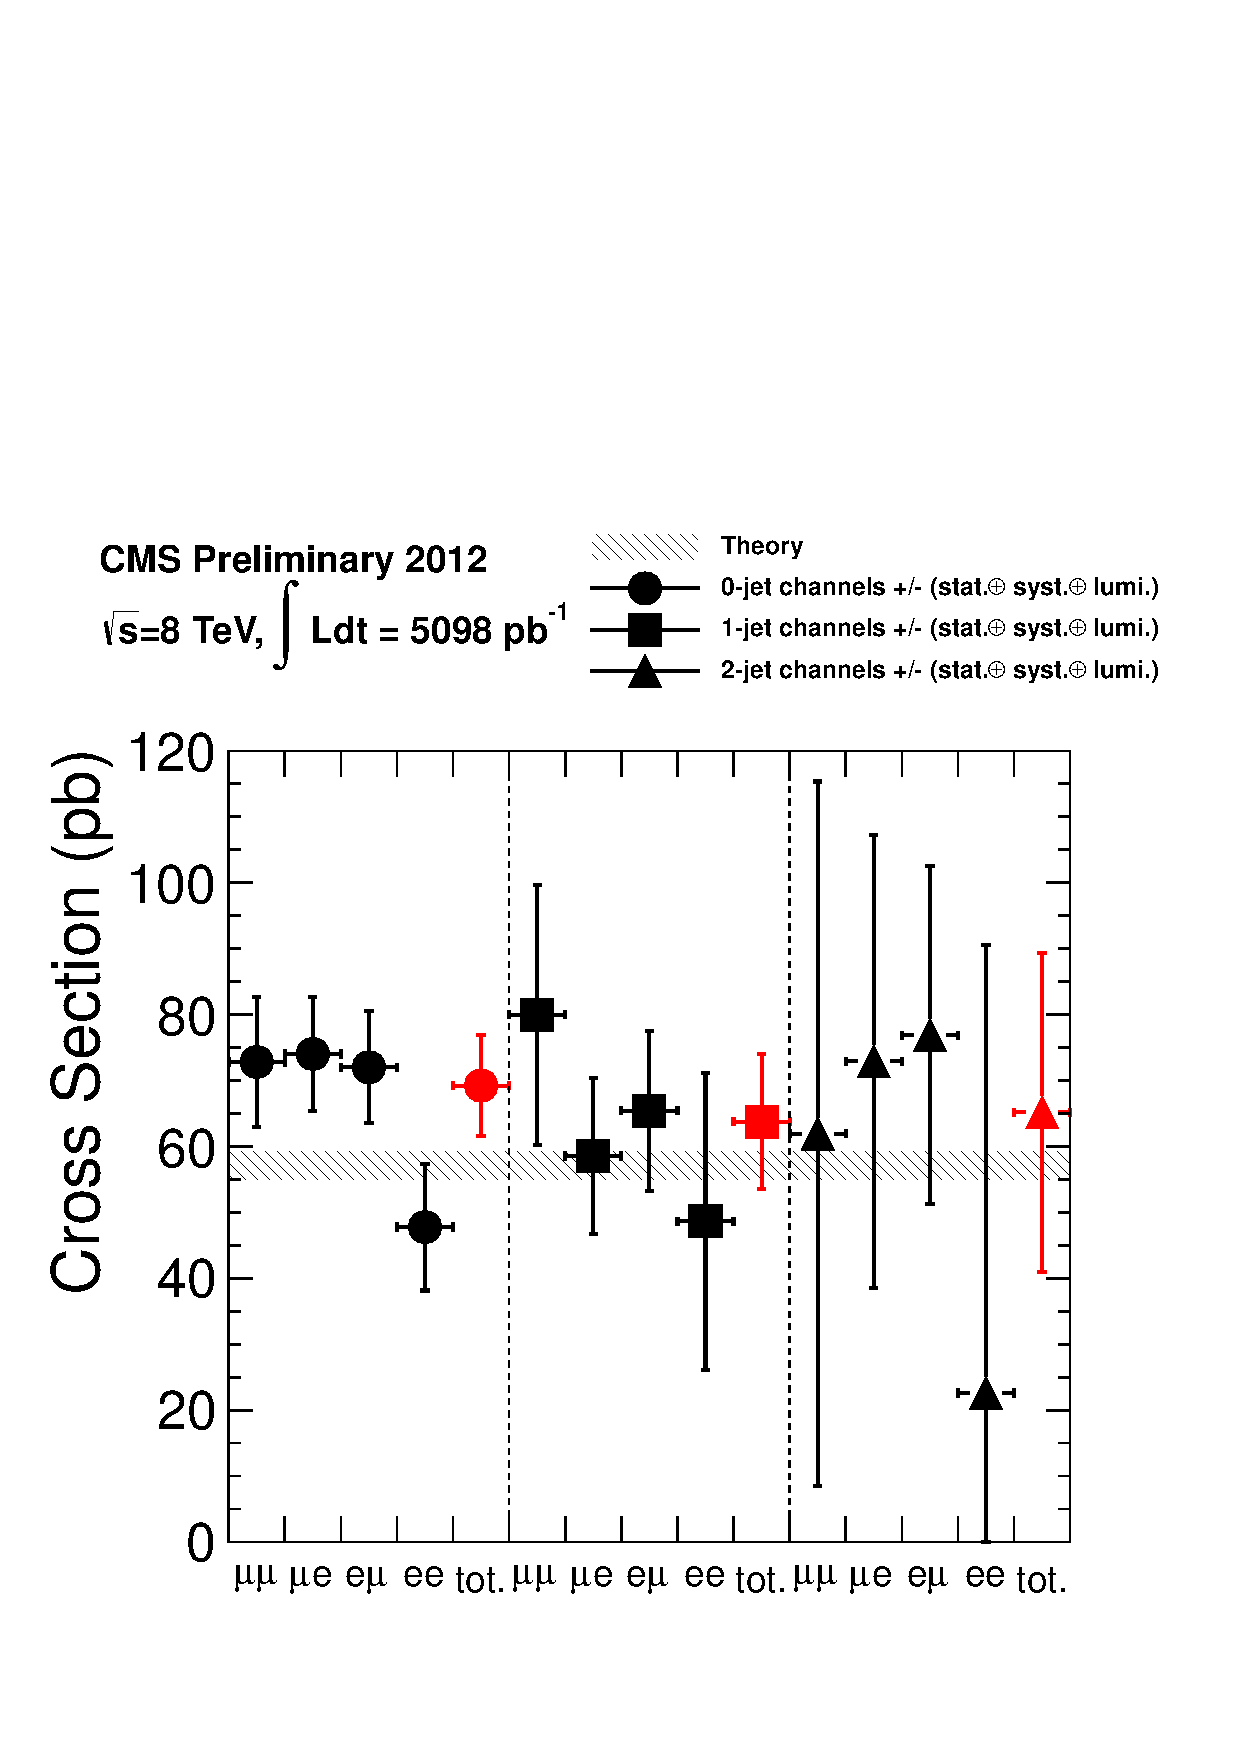
\includegraphics[width=.8\textwidth]{figures/ww_analysis20_0_summary.pdf}
\caption{Summary of all channels. Total uncertainty is shown.}
\label{fig:xs_summary_figure}
\end{figure}


\clearpage

\section{Cut-based Analysis results}

\subsection{Summary of Results (7+8 TeV) Combing all channels}

%%%%%%%%%%%%%%%%%%%%%%%%%%%%%%
\begin{figure}[!hbtp]
\centering
\subfigure[SM Higgs (cut-based) 7 TeV ]{
\centering
\label{subfig:sm_cut_7tev}
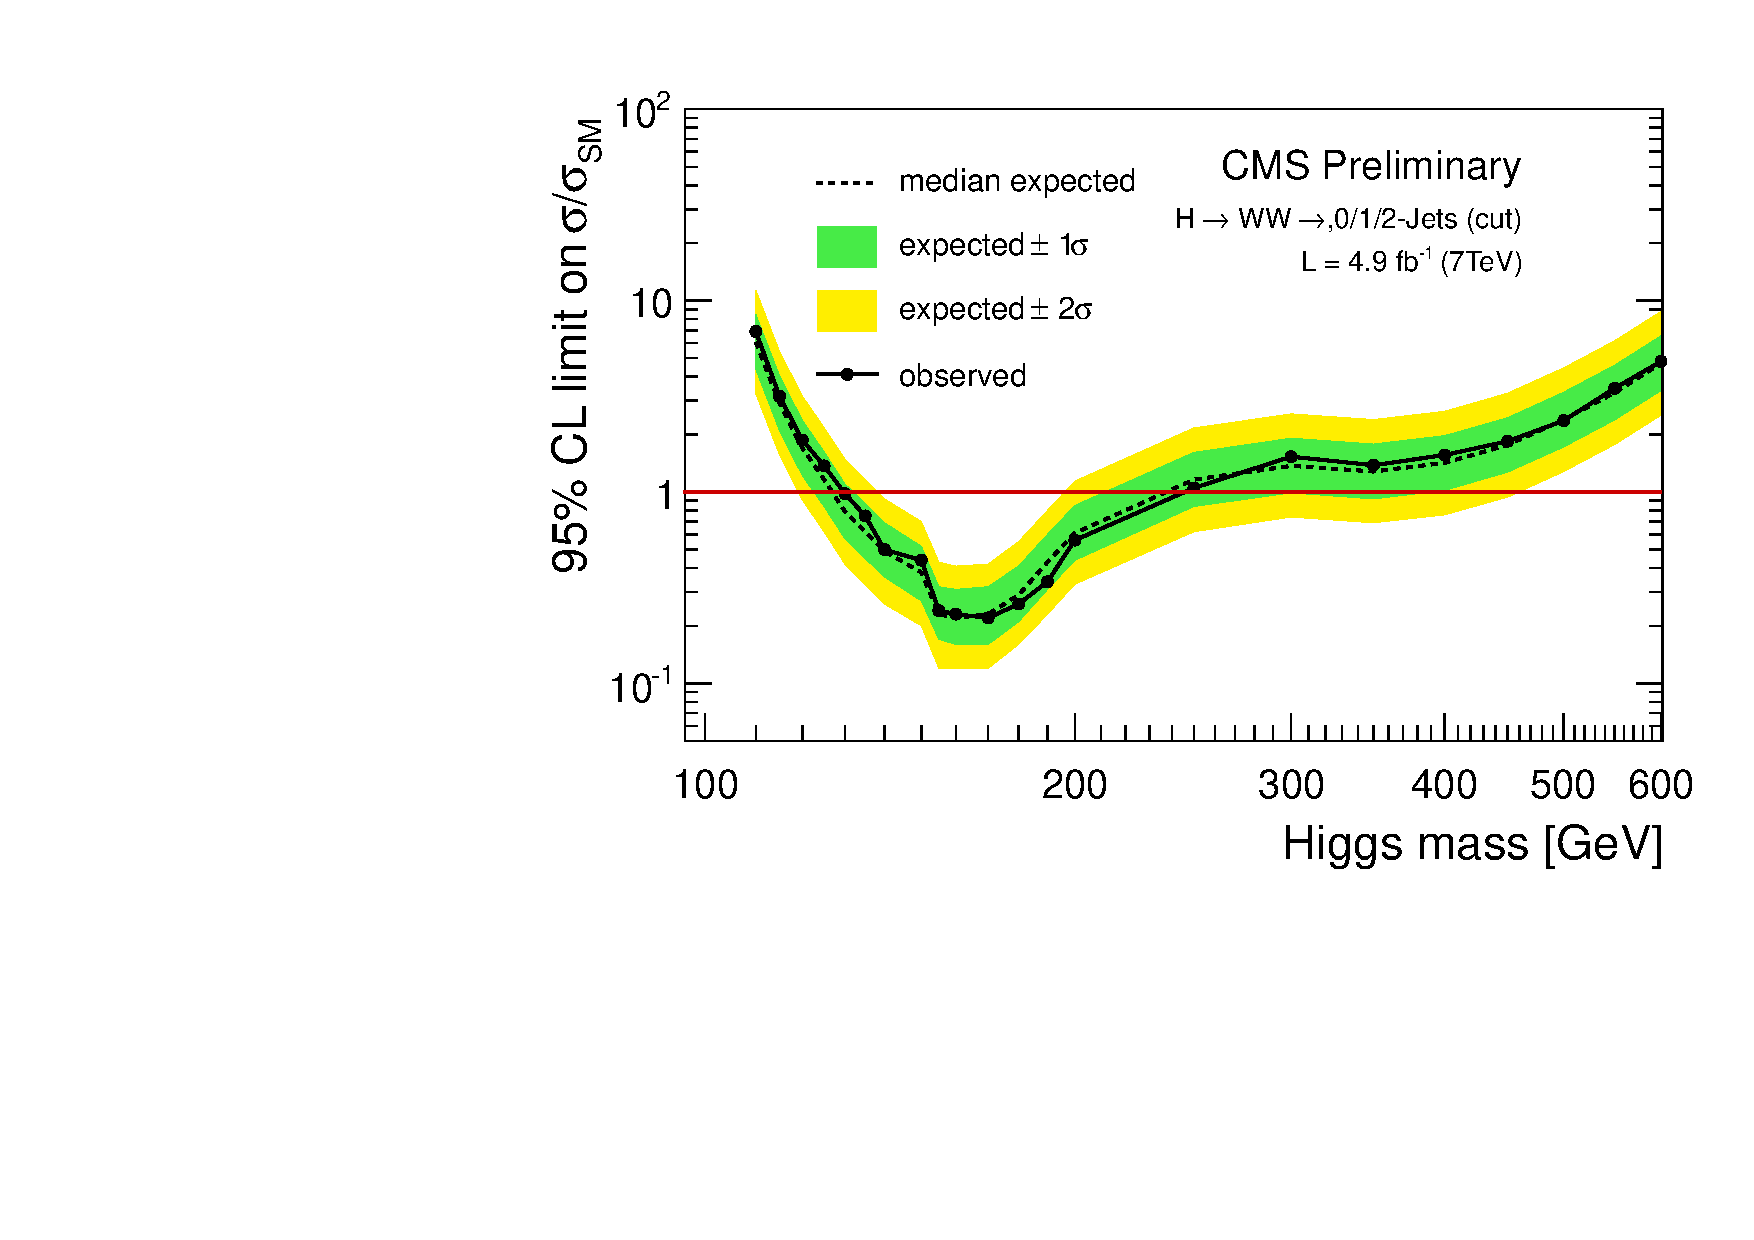
\includegraphics[width=.45\textwidth]{figures/limits_nj_cut_7TeV-CLs-asymptotic_log.pdf}}
\centering
\subfigure[SM Higgs (cut-based) 8 TeV ]{
\centering
\label{subfig:sm_cut_8tev}
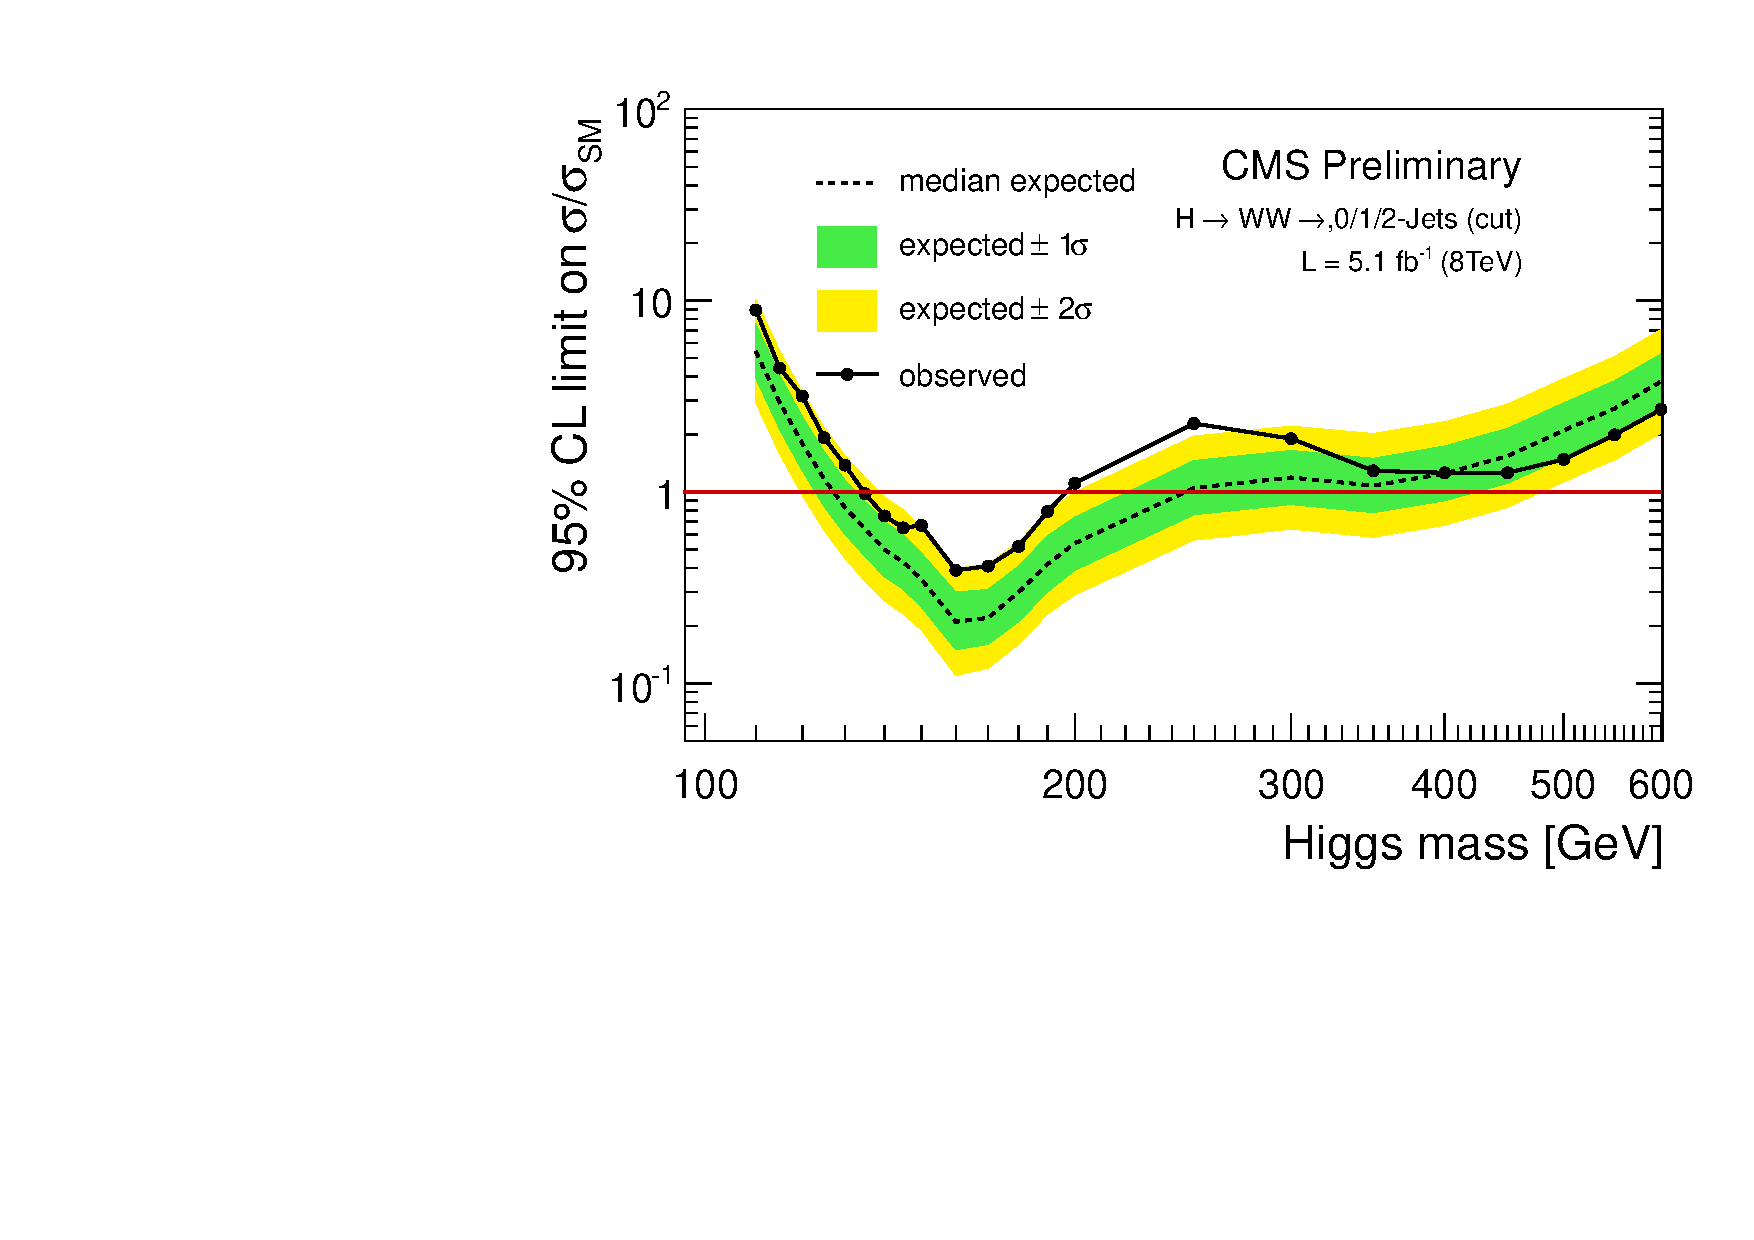
\includegraphics[width=.45\textwidth]{figures/limits_nj_cut_8TeV-CLs-asymptotic_log.pdf}} \\
\subfigure[SM Higgs (cut-based) 7+8 TeV ]{
\centering
\label{subfig:sm_cut_comb}
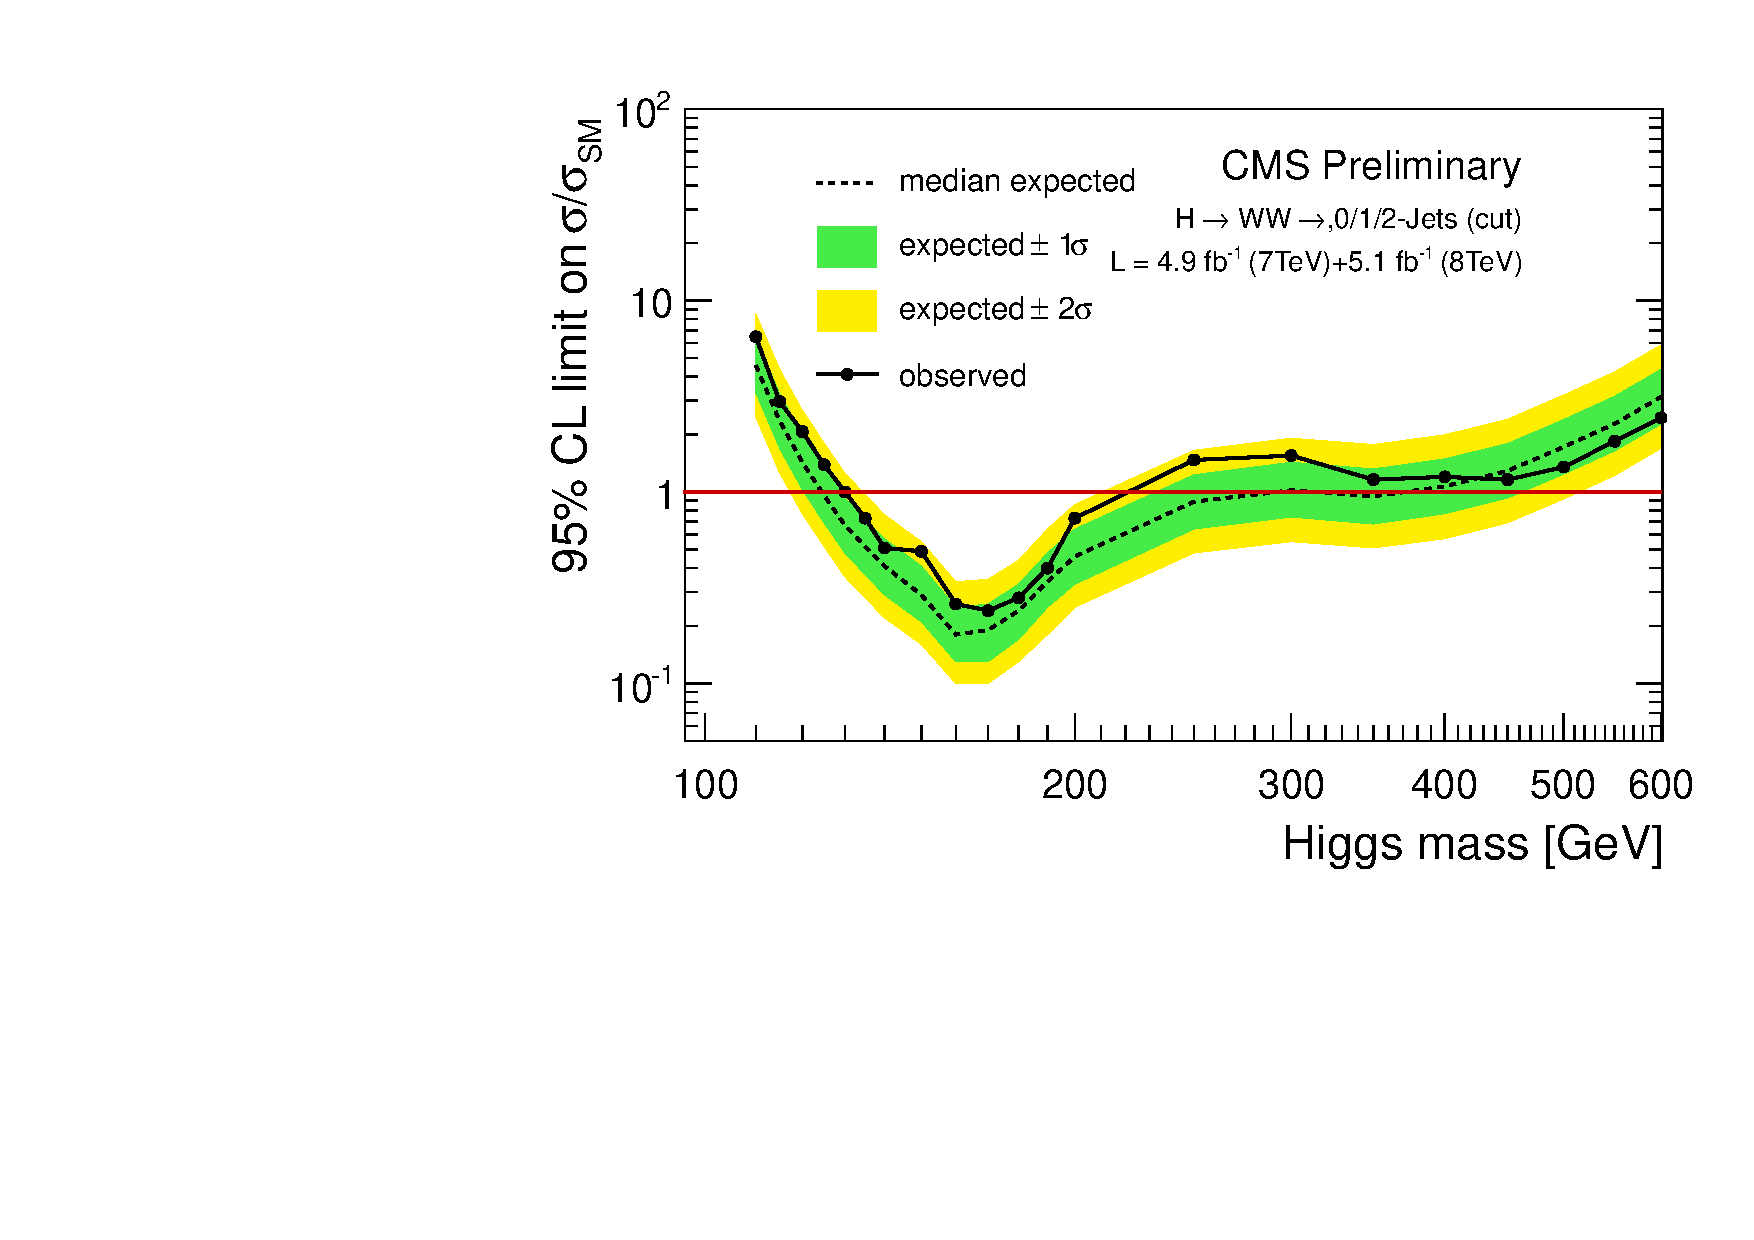
\includegraphics[width=.45\textwidth]{figures/limits_nj_cut-CLs-asymptotic_log.pdf}} \\ 
\label{fig:uls_cut}
\caption{Expected and observed upper limits for SM Higgs using the
  {\bf cut-based} analysis using 7 TeV, 8 TeV and combined data.}
\end{figure}



%%%%%%%%%%%%%%%%%%%%%%%%%%%%%%%%%%%%%%%%%%%%%%%%%%%%%%%%%%%%
\begin{table}[hbp!]
\begin{center}
\begin{tabular}{c c c c c}
\hline
\vspace{-3mm} && \\
 Higgs Mass & Observed  & Median expected & Expected range for 68\% & Expected range for 95\%   \\
\hline
\vspace{-3mm} && \\
110 & 6.89 & 6.07 & [4.37, 8.45] & [3.26, 11.33] \\
115 & 3.16 & 2.90 & [2.09, 4.04] & [1.56, 5.41] \\
120 & 1.87 & 1.70 & [1.22, 2.37] & [0.91, 3.17] \\
125 & 1.37 & 1.16 & [0.84, 1.62] & [0.62, 2.17] \\
130 & 0.98 & 0.79 & [0.57, 1.10] & [0.42, 1.48] \\
135 & 0.75 & 0.62 & [0.45, 0.87] & [0.33, 1.16] \\
140 & 0.50 & 0.49 & [0.36, 0.69] & [0.26, 0.92] \\
150 & 0.44 & 0.38 & [0.27, 0.52] & [0.20, 0.70] \\
160 & 0.23 & 0.22 & [0.16, 0.31] & [0.12, 0.41] \\
170 & 0.22 & 0.23 & [0.16, 0.32] & [0.12, 0.42] \\
180 & 0.26 & 0.29 & [0.21, 0.41] & [0.16, 0.55] \\
190 & 0.34 & 0.43 & [0.31, 0.60] & [0.23, 0.80] \\
200 & 0.56 & 0.61 & [0.44, 0.85] & [0.33, 1.14] \\
250 & 1.05 & 1.16 & [0.84, 1.61] & [0.62, 2.16] \\
300 & 1.53 & 1.37 & [0.99, 1.91] & [0.74, 2.56] \\
350 & 1.38 & 1.28 & [0.92, 1.78] & [0.69, 2.39] \\
400 & 1.56 & 1.42 & [1.02, 1.97] & [0.76, 2.64] \\
450 & 1.84 & 1.76 & [1.27, 2.44] & [0.94, 3.28] \\
500 & 2.36 & 2.39 & [1.72, 3.32] & [1.28, 4.45] \\
550 & 3.48 & 3.30 & [2.38, 4.59] & [1.77, 6.16] \\
600 & 4.81 & 4.70 & [3.39, 6.54] & [2.52, 8.77] \\
\hline
\end{tabular}
\caption{Expected and observed upper limits for SM Higgs using the
  {\bf cut-based} analysis, corresponding to $\intlumiSevenTeV$ at 7 TeV. }
\label{tab:cutbase_uls_7tev}
\end{center}
%\end{table}
%%%%%%%%%%%%%%%%%%%%%%%%%%%%%%
%\begin{table}[hbp!]
\begin{center}
\begin{tabular}{c c c c c}
\hline
\vspace{-3mm} && \\
 Higgs Mass & Observed  & Median expected & Expected range for 68\% & Expected range for 95\%   \\
\vspace{-3mm} && \\
\hline
110 & 8.92 & 5.43 & [3.91, 7.56] & [2.91, 10.13] \\
115 & 4.44 & 2.94 & [2.12, 4.09] & [1.58, 5.49] \\
120 & 3.17 & 1.79 & [1.29, 2.48] & [0.96, 3.33] \\
125 & 1.92 & 1.17 & [0.84, 1.63] & [0.63, 2.18] \\
130 & 1.38 & 0.83 & [0.60, 1.15] & [0.45, 1.55] \\
135 & 0.98 & 0.64 & [0.46, 0.89] & [0.34, 1.19] \\
140 & 0.75 & 0.50 & [0.36, 0.70] & [0.27, 0.94] \\
145 & 0.65 & 0.43 & [0.31, 0.60] & [0.23, 0.81] \\
150 & 0.67 & 0.35 & [0.25, 0.48] & [0.19, 0.65] \\
160 & 0.39 & 0.21 & [0.15, 0.30] & [0.11, 0.40] \\
170 & 0.41 & 0.22 & [0.16, 0.31] & [0.12, 0.42] \\
180 & 0.52 & 0.30 & [0.21, 0.41] & [0.16, 0.55] \\
190 & 0.79 & 0.42 & [0.30, 0.59] & [0.23, 0.79] \\
200 & 1.11 & 0.54 & [0.39, 0.74] & [0.29, 1.00] \\
250 & 2.28 & 1.05 & [0.76, 1.46] & [0.56, 1.96] \\
300 & 1.90 & 1.19 & [0.86, 1.65] & [0.64, 2.21] \\
350 & 1.29 & 1.08 & [0.78, 1.50] & [0.58, 2.02] \\
400 & 1.26 & 1.25 & [0.90, 1.74] & [0.67, 2.33] \\
450 & 1.26 & 1.54 & [1.11, 2.15] & [0.83, 2.88] \\
500 & 1.48 & 2.10 & [1.51, 2.92] & [1.13, 3.91] \\
550 & 1.99 & 2.73 & [1.97, 3.81] & [1.47, 5.10] \\
600 & 2.70 & 3.78 & [2.73, 5.26] & [2.03, 7.06] \\
\hline
\end{tabular}
\caption{Expected and observed upper limits for SM Higgs using the
  {\bf cut-based} analysis with \intlumiEightTeV\ of data at 8 TeV.}
\label{tab:cutbase_uls_8tev}
\end{center}
\end{table}
%%%%%%%%%%%%%%%%%%%%%%%%%%%%%%
\begin{table}[hbp!]
\begin{center}
\begin{tabular}{c c c c c}
\hline
\vspace{-3mm} && \\
 Higgs Mass & Observed  & Median expected & Expected range for 68\% & Expected range for 95\%   \\
\hline
\vspace{-3mm} && \\
110 & 6.47 & 4.58 & [3.30, 6.37] & [2.46, 8.54] \\
115 & 2.97 & 2.35 & [1.69, 3.27] & [1.26, 4.38] \\
120 & 2.07 & 1.43 & [1.03, 1.99] & [0.77, 2.67] \\
125 & 1.39 & 0.96 & [0.69, 1.34] & [0.52, 1.80] \\
130 & 1.00 & 0.67 & [0.48, 0.93] & [0.36, 1.25] \\
135 & 0.73 & 0.52 & [0.37, 0.72] & [0.28, 0.97] \\
140 & 0.51 & 0.41 & [0.29, 0.57] & [0.22, 0.76] \\
150 & 0.49 & 0.29 & [0.21, 0.41] & [0.16, 0.55] \\
160 & 0.26 & 0.18 & [0.13, 0.25] & [0.10, 0.34] \\
170 & 0.24 & 0.19 & [0.13, 0.26] & [0.10, 0.35] \\
180 & 0.28 & 0.24 & [0.17, 0.33] & [0.13, 0.44] \\
190 & 0.40 & 0.34 & [0.25, 0.48] & [0.18, 0.64] \\
200 & 0.73 & 0.46 & [0.33, 0.64] & [0.25, 0.86] \\
250 & 1.47 & 0.89 & [0.64, 1.23] & [0.48, 1.65] \\
300 & 1.55 & 1.02 & [0.74, 1.43] & [0.55, 1.91] \\
350 & 1.16 & 0.95 & [0.68, 1.32] & [0.51, 1.77] \\
400 & 1.20 & 1.07 & [0.77, 1.49] & [0.57, 1.99] \\
450 & 1.16 & 1.29 & [0.93, 1.79] & [0.69, 2.40] \\
500 & 1.35 & 1.72 & [1.24, 2.39] & [0.92, 3.21] \\
550 & 1.84 & 2.27 & [1.64, 3.16] & [1.22, 4.24] \\
600 & 2.44 & 3.14 & [2.26, 4.37] & [1.69, 5.86] \\
\hline
\end{tabular}
\caption{Expected and observed upper limits for SM Higgs using the
  {\bf cut-based} analysis, corresponding to $\intlumiSevenTeV$ at 7 TeV and $\intlumiEightTeV$ 8 TeV data.}
\label{tab:cutbase_uls_7and8tev}
\end{center}
\end{table}
%%%%%%%%%%%%%%%%%%%%%%%%%%%%%
\clearpage


\subsection{Combine 7 TeV and 8 TeV OF}



%%%%%%%%%%%%%%%%%%%%%%%%%%%%%%%%%%%%%%%%%%%%%%%%%%%%%%%%%%%%
\begin{table}[hbp!]
\begin{center}
\begin{tabular}{c c c c c}
\hline
\vspace{-3mm} && \\
 Higgs Mass & Observed  & Median expected & Expected range for 68\% & Expected range for 95\%   \\
\hline
\vspace{-3mm} && \\
110 & 8.81 & 6.25 & [4.50, 8.70] & [3.35, 11.66] \\
115 & 4.76 & 3.29 & [2.37, 4.58] & [1.77, 6.14] \\
120 & 3.14 & 1.98 & [1.43, 2.75] & [1.06, 3.69] \\
125 & 1.95 & 1.29 & [0.93, 1.79] & [0.69, 2.40] \\
130 & 1.39 & 0.93 & [0.67, 1.29] & [0.50, 1.73] \\
135 & 0.99 & 0.69 & [0.50, 0.96] & [0.37, 1.29] \\
140 & 0.76 & 0.56 & [0.40, 0.78] & [0.30, 1.05] \\
145 & 0.70 & 0.48 & [0.35, 0.67] & [0.26, 0.90] \\
150 & 0.56 & 0.38 & [0.27, 0.53] & [0.20, 0.71] \\
160 & 0.37 & 0.23 & [0.16, 0.31] & [0.12, 0.42] \\
170 & 0.34 & 0.25 & [0.18, 0.34] & [0.13, 0.46] \\
180 & 0.43 & 0.33 & [0.24, 0.46] & [0.18, 0.62] \\
190 & 0.69 & 0.52 & [0.37, 0.72] & [0.28, 0.97] \\
200 & 0.95 & 0.65 & [0.47, 0.91] & [0.35, 1.21] \\
250 & 2.21 & 1.24 & [0.90, 1.73] & [0.67, 2.32] \\
300 & 2.31 & 1.46 & [1.05, 2.03] & [0.78, 2.73] \\
350 & 1.47 & 1.29 & [0.93, 1.80] & [0.69, 2.41] \\
400 & 1.57 & 1.46 & [1.05, 2.03] & [0.78, 2.72] \\
450 & 1.64 & 1.83 & [1.32, 2.55] & [0.98, 3.41] \\
500 & 1.79 & 2.45 & [1.76, 3.41] & [1.31, 4.57] \\
550 & 2.33 & 3.30 & [2.38, 4.59] & [1.77, 6.16] \\
600 & 3.15 & 4.74 & [3.42, 6.60] & [2.55, 8.85] \\
\hline
\end{tabular}
\caption{Expected and observed upper limits for SM Higgs using the
  {\bf cut-based} analysis, using the OF channels in the 0/1-Jet bin in the 8 TeV data ($\intlumiEightTeV$). }
\label{tab:bdtbase_uls_7tev_8tevof}
\end{center}
%\end{table}
%%%%%%%%%%%%%%%%%%%%%%%%%%%%%%

%%%%%%%%%%%%%%%%%%%%%%%%%%%%%%%%%%%%%%%%%%%%%%%%%%%%%%%%%%%%
%\begin{table}[hbp!]
\begin{center}
\begin{tabular}{c c c c c}
\hline
\vspace{-3mm} && \\
 Higgs Mass & Observed  & Median expected & Expected range for 68\% & Expected range for 95\%   \\
\hline
\vspace{-3mm} && \\


\hline
\end{tabular}
\caption{Expected and observed upper limits for SM Higgs using the
  {\bf shape-based} analysis using the OF channels in the 0/1-Jet bin in the 8 TeV data ($\intlumiEightTeV$). }
\label{tab:bdtbase_uls_8tevof}
\end{center}
\end{table}
%%%%%%%%%%%%%%%%%%%%%%%%%%%%%%



%%%%%%%%%%%%%%%%%%%%%%%%%%%%%%%%%%%%%%%%%%%%%%%%%%%%%%%%%%%%
\begin{table}[hbp!]
\begin{center}
\begin{tabular}{c c c c c}
\hline
\vspace{-3mm} && \\
 Higgs Mass & Observed  & Median expected & Expected range for 68\% & Expected range for 95\%   \\
\hline
\vspace{-3mm} && \\


\hline
\end{tabular}
\caption{Expected and observed upper limits for SM Higgs using the
  {\bf cut-based} analysis, combining the 7 TeV data using all channels ($\intlumiSevenTeV$) 
and the OF channels in the 0/1-Jet bin in the 8 TeV data ($\intlumiEightTeV$). }
\label{tab:cutbase_uls_7tev_8tevof}
\end{center}
%\end{table}
%%%%%%%%%%%%%%%%%%%%%%%%%%%%%%

%%%%%%%%%%%%%%%%%%%%%%%%%%%%%%%%%%%%%%%%%%%%%%%%%%%%%%%%%%%%
%\begin{table}[hbp!]
\begin{center}
\begin{tabular}{c c c c c}
\hline
\vspace{-3mm} && \\
 Higgs Mass & Observed  & Median expected & Expected range for 68\% & Expected range for 95\%   \\
\hline
\vspace{-3mm} && \\


\hline
\end{tabular}
\caption{Expected and observed upper limits for SM Higgs using the
  {\bf shape-based} analysis, combining the 7 TeV data using all channels ($\intlumiSevenTeV$) 
and the OF channels in the 0/1-Jet bin in the 8 TeV data ($\intlumiEightTeV$). }
\label{tab:bdtbase_uls_7tev_8tevof}
\end{center}
\end{table}
%%%%%%%%%%%%%%%%%%%%%%%%%%%%%%

\clearpage

\subsection{Detailed Results at 8 TeV}

%%%%%%%%%%%%%%%%%%%%%%%%%%%%%%
\begin{figure}[!hbtp]
\centering
\subfigure[SM Higgs (cut-based) 8 TeV 0-Jet OF ]{
\centering
\label{subfig:sm_cut_8tev_0jof}
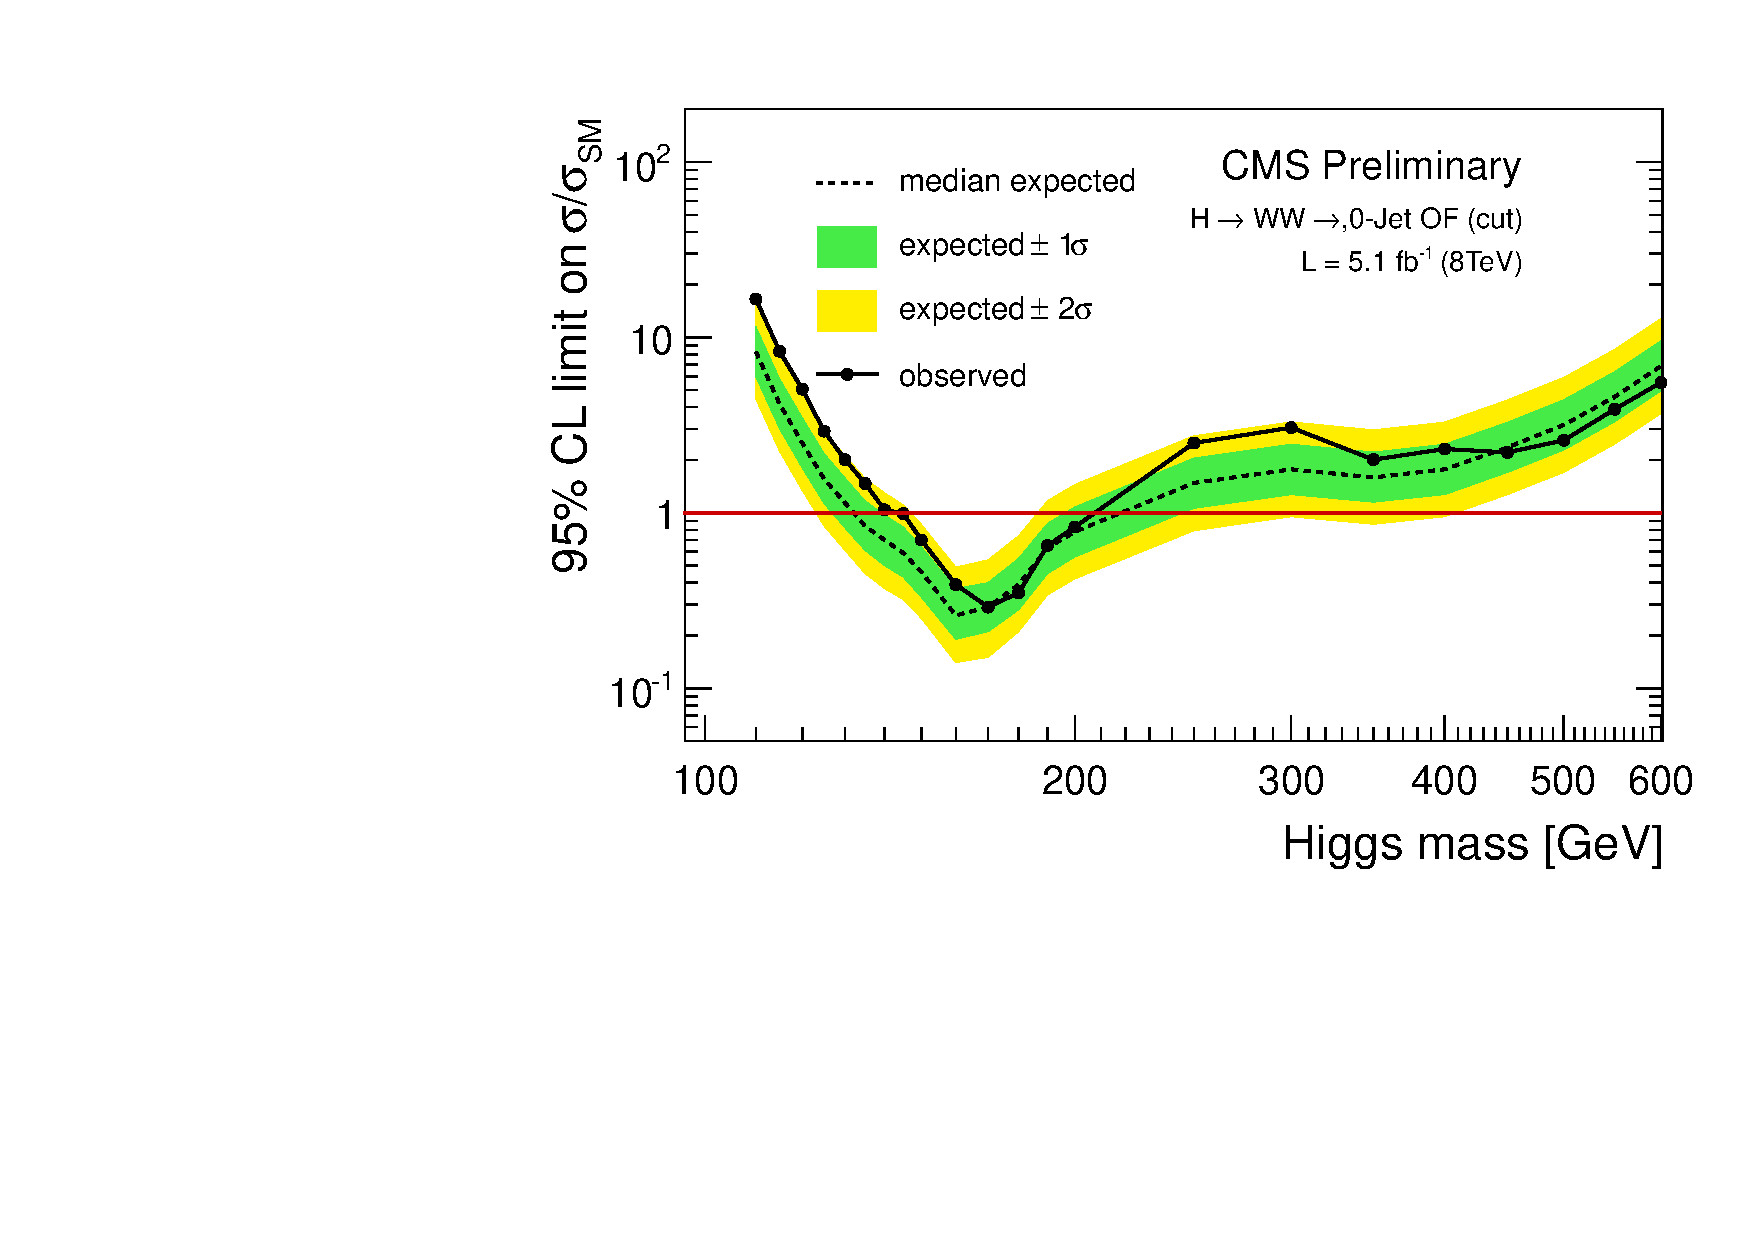
\includegraphics[width=.45\textwidth]{figures/limits_0jof_cut_8TeV-CLs-asymptotic_log.pdf}}
\subfigure[SM Higgs (cut-based) 8 TeV 0-Jet SF ]{
\centering
\label{subfig:sm_cut_8tev_0jof}
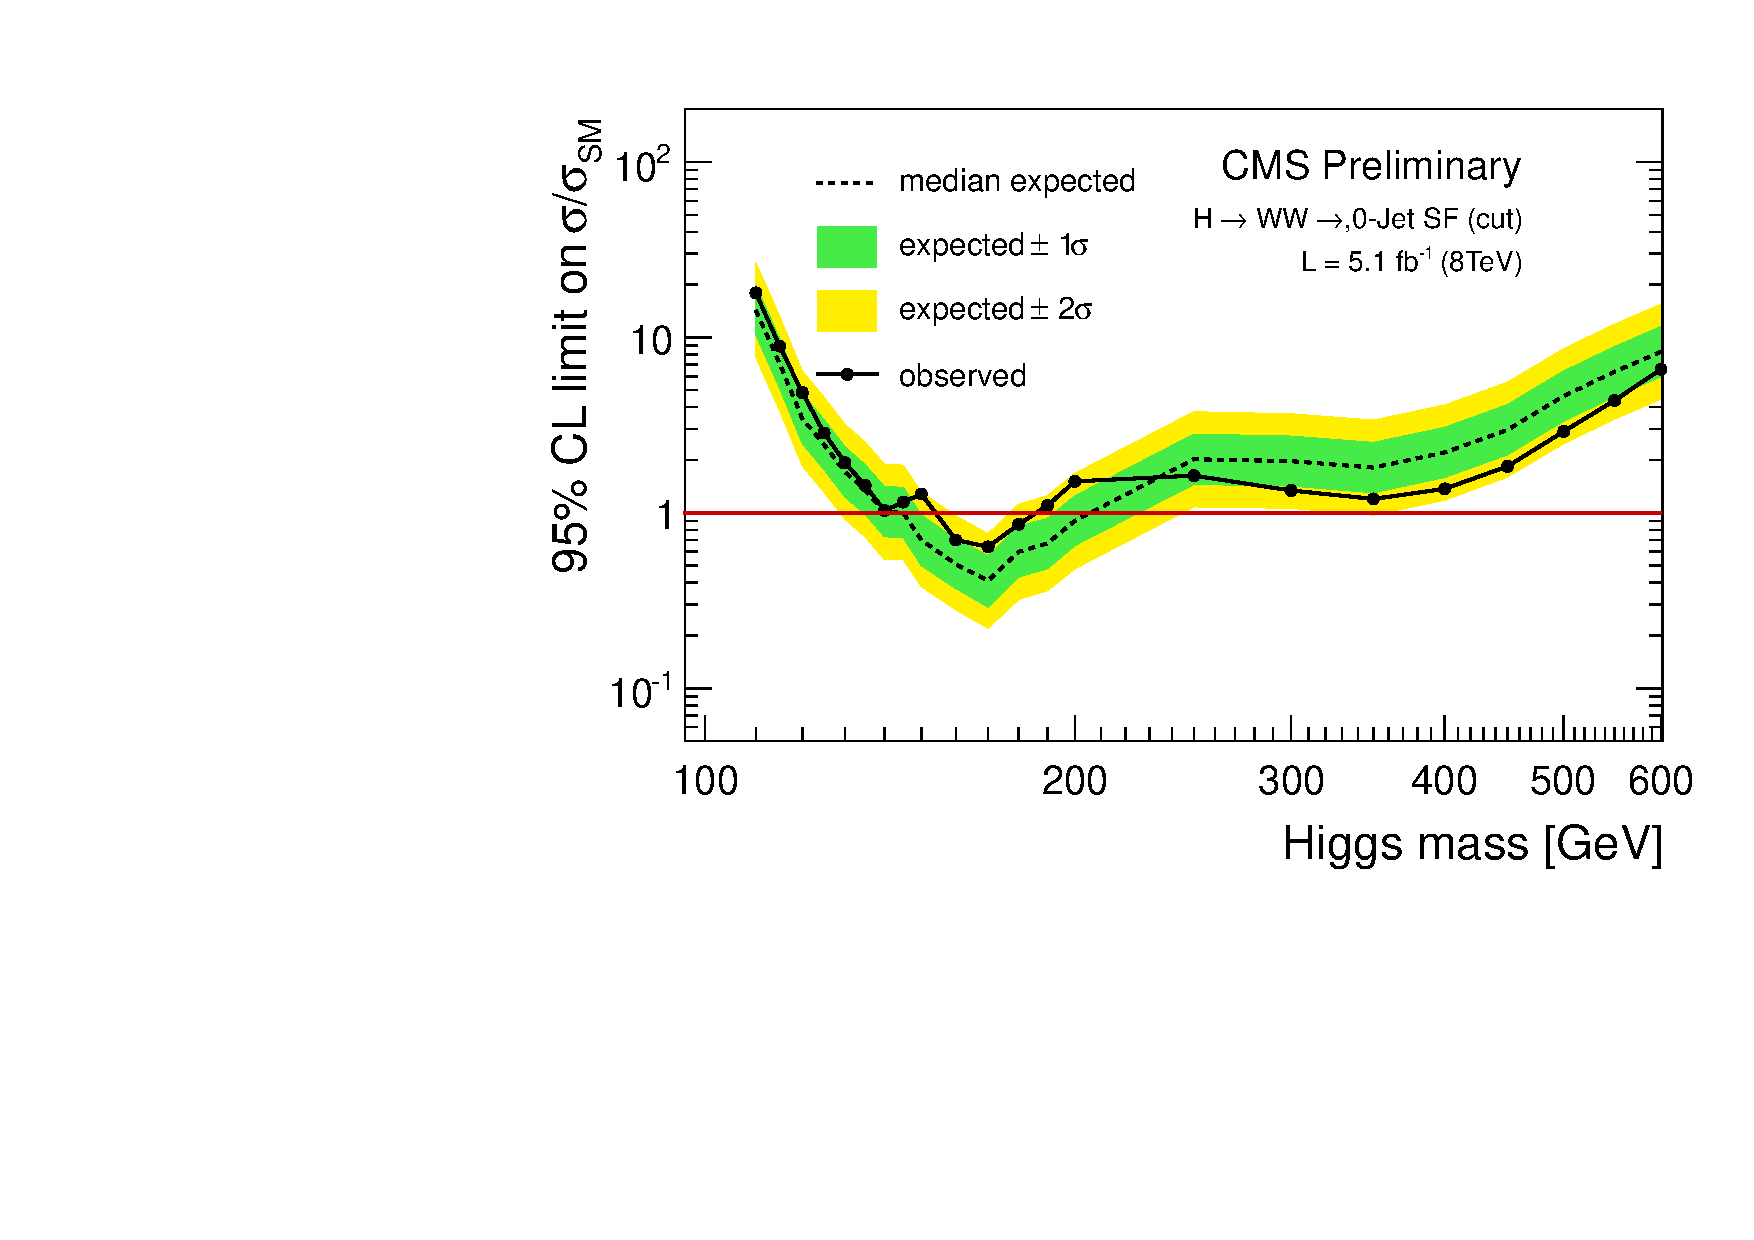
\includegraphics[width=.45\textwidth]{figures/limits_0jsf_cut_8TeV-CLs-asymptotic_log.pdf}} \\
\subfigure[SM Higgs (cut-based) 8 TeV 1-Jet OF ]{
\centering
\label{subfig:sm_cut_8tev_0jof}
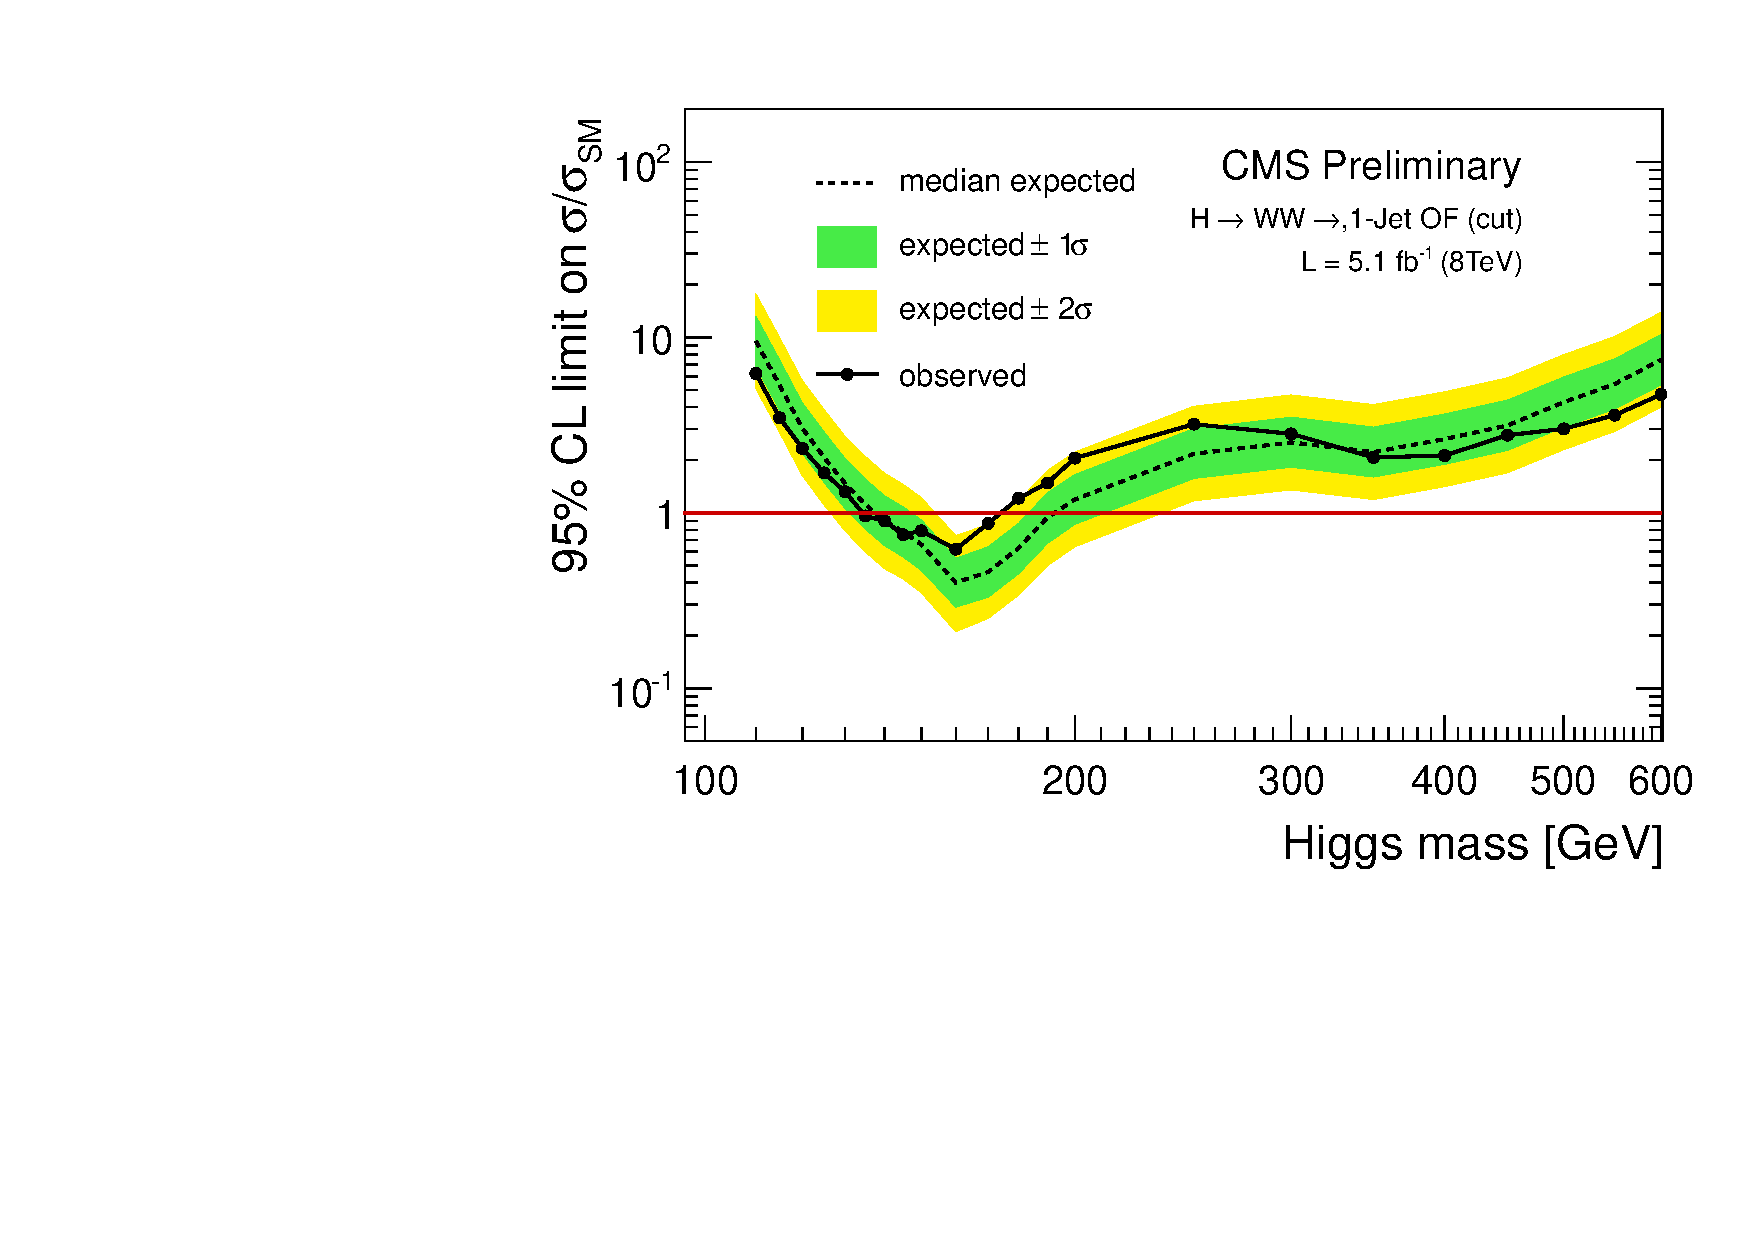
\includegraphics[width=.45\textwidth]{figures/limits_1jof_cut_8TeV-CLs-asymptotic_log.pdf}}
\subfigure[SM Higgs (cut-based) 8 TeV 1-Jet SF ]{
\centering
\label{subfig:sm_cut_8tev_0jof}
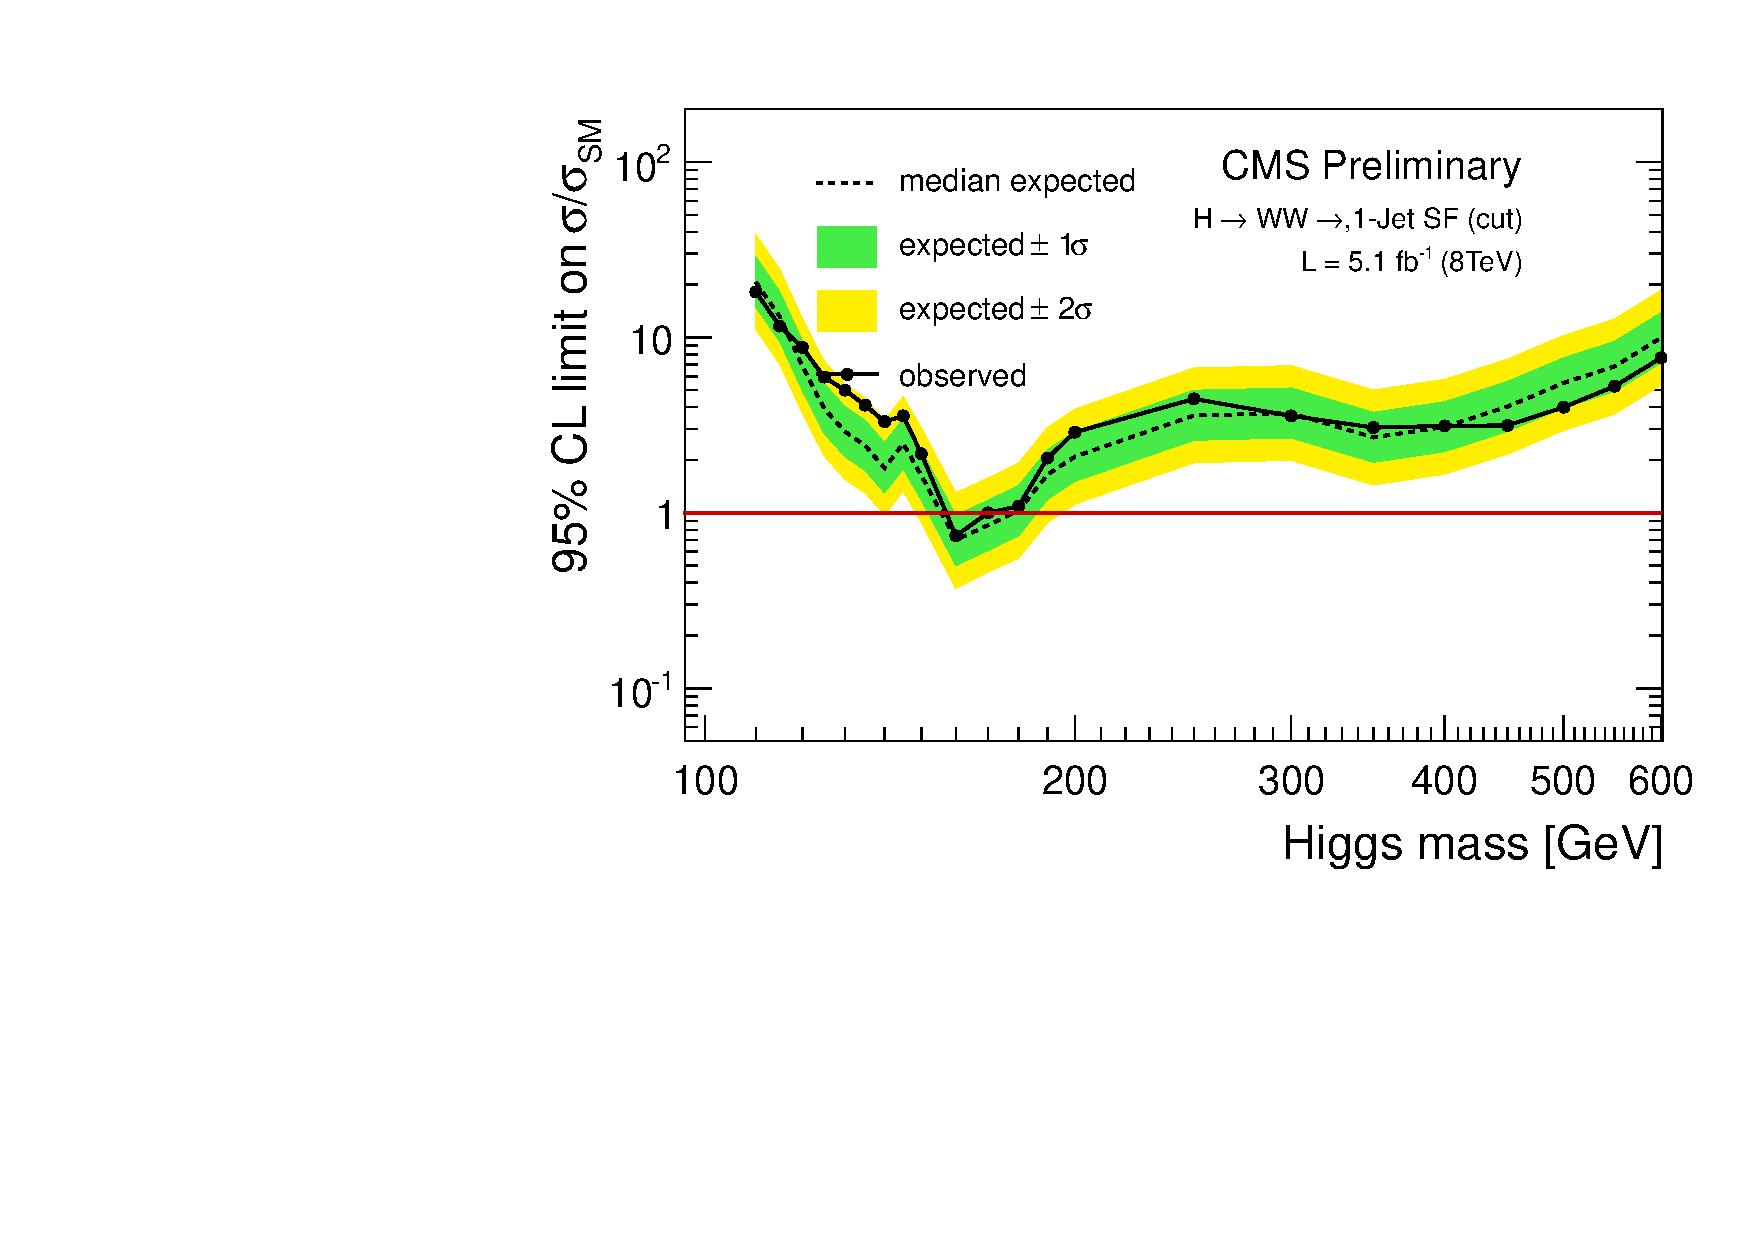
\includegraphics[width=.45\textwidth]{figures/limits_1jsf_cut_8TeV-CLs-asymptotic_log.pdf}} \\
\subfigure[SM Higgs (cut-based) 8 TeV 2-Jet OF ]{
\centering
\label{subfig:sm_cut_8tev_0jof}
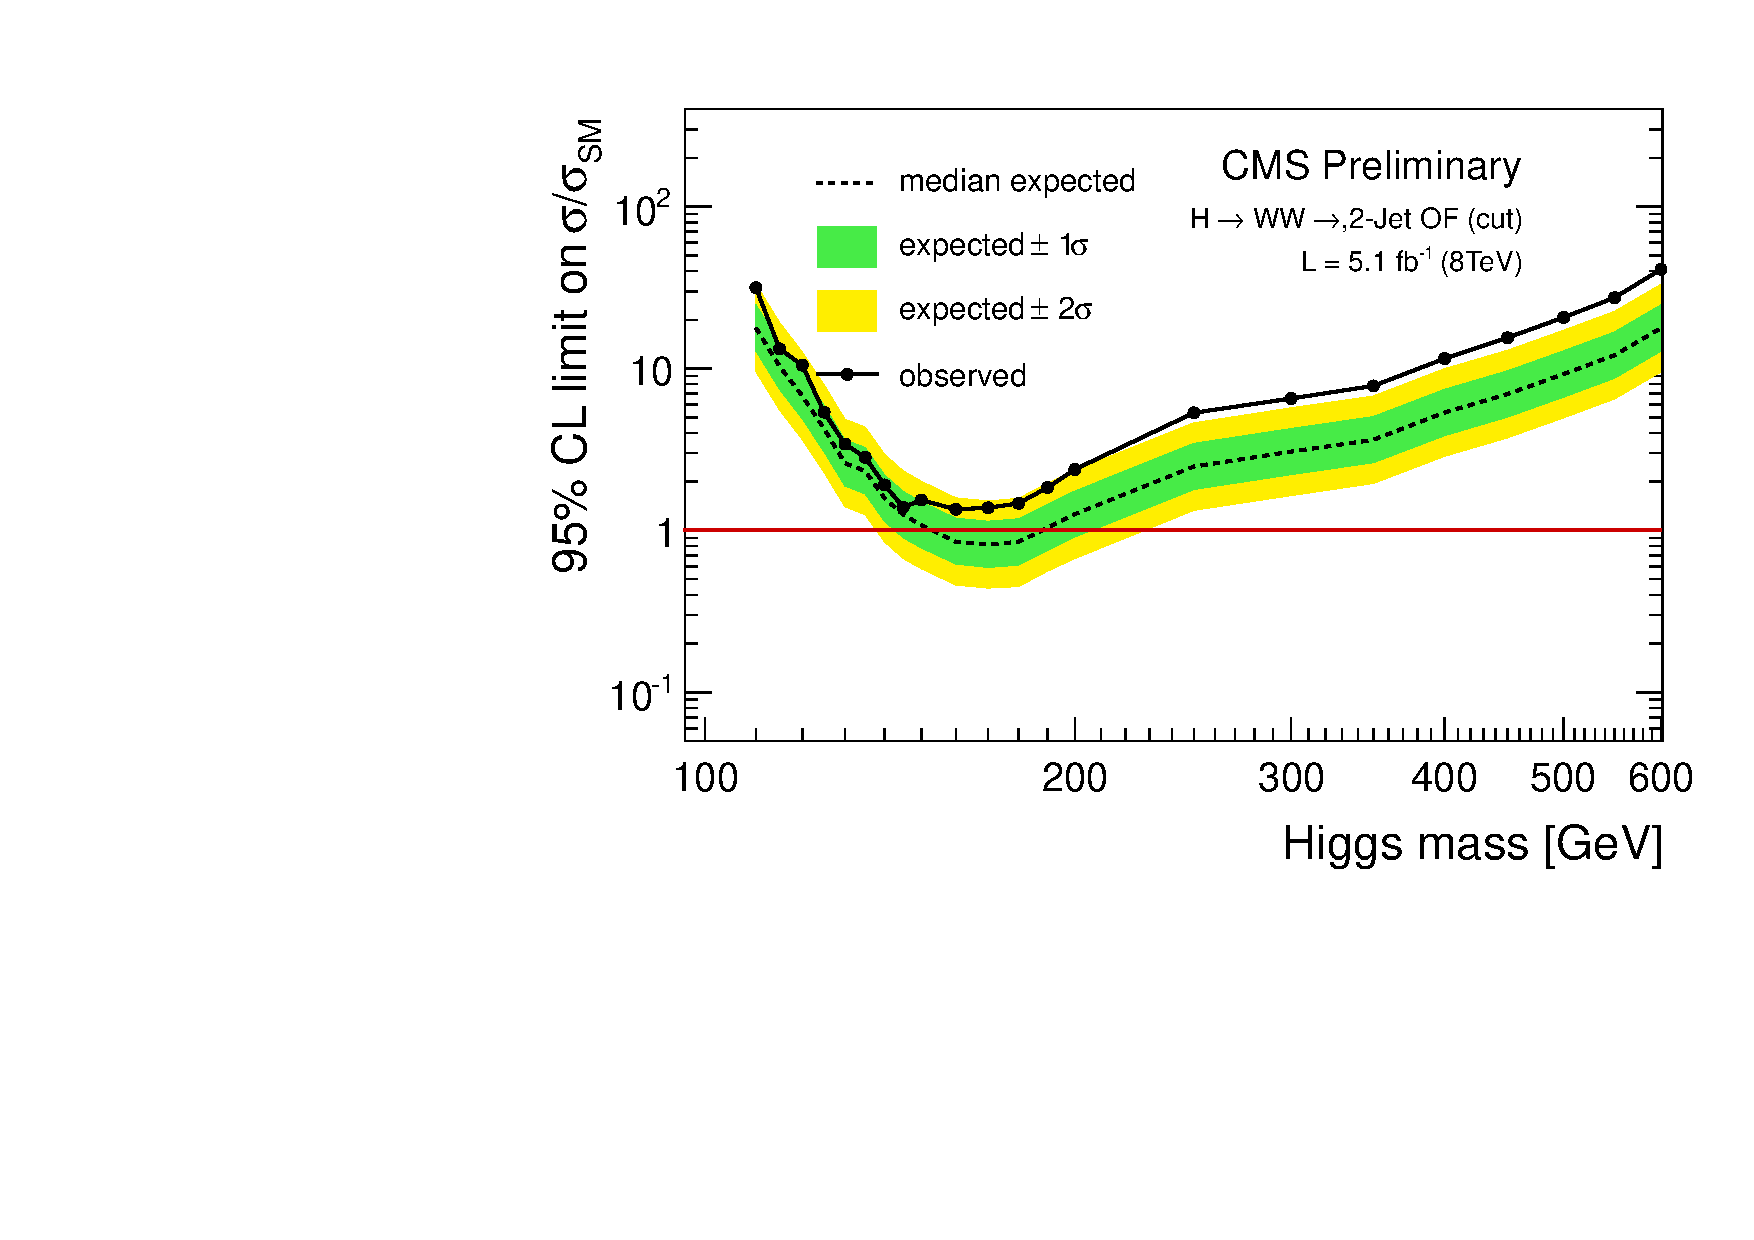
\includegraphics[width=.45\textwidth]{figures/limits_2jof_cut_8TeV-CLs-asymptotic_log.pdf}}
\subfigure[SM Higgs (cut-based) 8 TeV 2-Jet SF ]{
\centering
\label{subfig:sm_cut_8tev_0jof}
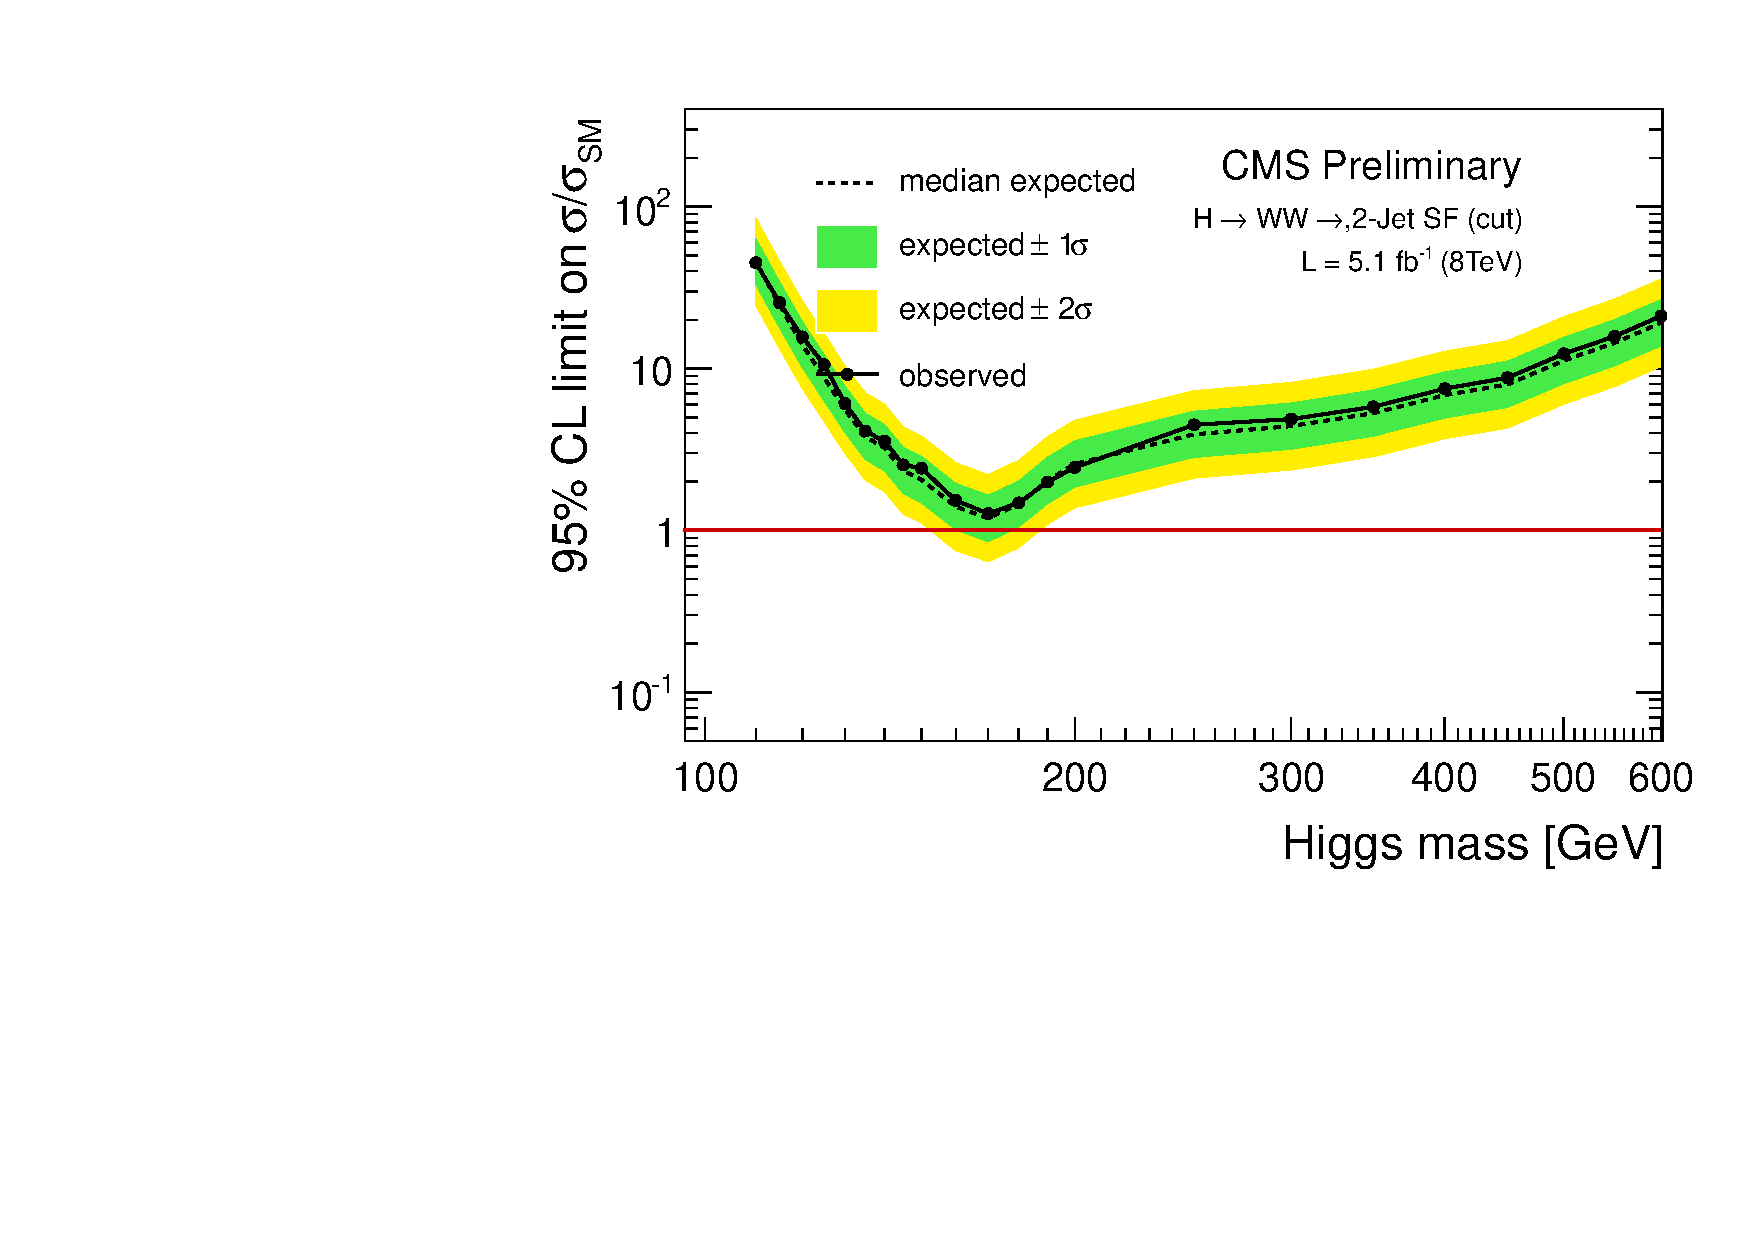
\includegraphics[width=.45\textwidth]{figures/limits_2jsf_cut_8TeV-CLs-asymptotic_log.pdf}} \\
\label{fig:uls_cut_8tev}
\caption{Expected and observed upper limits for SM Higgs using the
  {\bf cut-based} analysis using {\bf 8 TeV data}.}
\end{figure}
%%%%%%%%%%%%%%%%%%%%%%%%%%%%%%%%%%%%%%%%%%%%%%%%%%%%%%%%%%%%
%%%%%%%%%%%%%%%%%%%%%%%%%%%%%%
\begin{table}[hbp!]
\begin{center}
\begin{tabular}{c c c c c}
\hline
\vspace{-3mm} && \\
 Higgs Mass & Observed  & Median expected & Expected range for 68\% & Expected range for 95\%   \\
\vspace{-3mm} && \\
\hline
\multicolumn{5}{c}{0-Jet OF} \\
\hline
110 & 16.54 & 8.28 & [5.96, 11.52] & [4.44, 15.44] \\
115 & 8.33 & 4.17 & [3.01, 5.81] & [2.24, 7.79] \\
120 & 5.07 & 2.50 & [1.80, 3.48] & [1.34, 4.67] \\
125 & 2.92 & 1.56 & [1.13, 2.18] & [0.84, 2.92] \\
130 & 2.01 & 1.14 & [0.82, 1.58] & [0.61, 2.12] \\
135 & 1.47 & 0.84 & [0.61, 1.17] & [0.45, 1.57] \\
140 & 1.04 & 0.70 & [0.50, 0.97] & [0.37, 1.30] \\
145 & 0.99 & 0.59 & [0.43, 0.83] & [0.32, 1.11] \\
150 & 0.70 & 0.46 & [0.33, 0.64] & [0.25, 0.86] \\
160 & 0.39 & 0.26 & [0.19, 0.37] & [0.14, 0.49] \\
170 & 0.29 & 0.29 & [0.21, 0.40] & [0.15, 0.54] \\
180 & 0.35 & 0.39 & [0.28, 0.55] & [0.21, 0.74] \\
190 & 0.65 & 0.63 & [0.45, 0.87] & [0.34, 1.17] \\
200 & 0.83 & 0.78 & [0.56, 1.08] & [0.42, 1.45] \\
250 & 2.50 & 1.48 & [1.06, 2.05] & [0.79, 2.75] \\
300 & 3.06 & 1.77 & [1.27, 2.46] & [0.95, 3.30] \\
350 & 2.01 & 1.59 & [1.15, 2.22] & [0.86, 2.97] \\
400 & 2.31 & 1.77 & [1.27, 2.46] & [0.95, 3.29] \\
450 & 2.21 & 2.36 & [1.70, 3.28] & [1.27, 4.40] \\
500 & 2.59 & 3.17 & [2.28, 4.41] & [1.70, 5.91] \\
550 & 3.89 & 4.58 & [3.30, 6.37] & [2.46, 8.54] \\
600 & 5.53 & 6.86 & [4.95, 9.55] & [3.68, 12.81] \\
110 & 17.93 & 14.28 & [10.29, 19.87] & [7.66, 26.64] \\
\hline
\multicolumn{5}{c}{0-Jet SF} \\
\hline
115 & 8.92 & 7.11 & [5.12, 9.89] & [3.82, 13.26] \\
120 & 4.85 & 3.45 & [2.48, 4.80] & [1.85, 6.43] \\
125 & 2.85 & 2.45 & [1.76, 3.40] & [1.31, 4.56] \\
130 & 1.93 & 1.71 & [1.23, 2.38] & [0.92, 3.19] \\
135 & 1.43 & 1.35 & [0.98, 1.88] & [0.73, 2.53] \\
140 & 1.03 & 1.01 & [0.73, 1.41] & [0.54, 1.89] \\
145 & 1.15 & 1.00 & [0.72, 1.40] & [0.54, 1.87] \\
150 & 1.28 & 0.70 & [0.50, 0.97] & [0.38, 1.31] \\
160 & 0.70 & 0.51 & [0.37, 0.71] & [0.28, 0.96] \\
170 & 0.64 & 0.41 & [0.29, 0.57] & [0.22, 0.76] \\
180 & 0.86 & 0.60 & [0.43, 0.84] & [0.32, 1.12] \\
190 & 1.10 & 0.67 & [0.48, 0.93] & [0.36, 1.25] \\
200 & 1.51 & 0.90 & [0.65, 1.25] & [0.48, 1.68] \\
250 & 1.63 & 2.02 & [1.45, 2.81] & [1.08, 3.77] \\
300 & 1.34 & 1.97 & [1.42, 2.74] & [1.06, 3.67] \\
350 & 1.20 & 1.81 & [1.30, 2.52] & [0.97, 3.38] \\
400 & 1.37 & 2.21 & [1.59, 3.07] & [1.18, 4.12] \\
450 & 1.84 & 2.97 & [2.14, 4.14] & [1.60, 5.55] \\
500 & 2.91 & 4.63 & [3.33, 6.44] & [2.48, 8.63] \\
550 & 4.37 & 6.37 & [4.59, 8.87] & [3.42, 11.89] \\
600 & 6.58 & 8.29 & [5.97, 11.54] & [4.45, 15.47] \\

\hline
\end{tabular}
\caption{Expected and observed upper limits for SM Higgs using the
  {\bf cut-based} analysis with \intlumiEightTeV\ of data in the {\bf 0-Jet} final state.}
\label{tab:cutbase_uls_0j}
\end{center}
\end{table}
%%%%%%%%%%%%%%%%%%%%%%%%%%%%%%

%%%%%%%%%%%%%%%%%%%%%%%%%%%%%%%%%%%%%%%%%%%%%%%%%%%%%%%%%%%%
%%%%%%%%%%%%%%%%%%%%%%%%%%%%%%
\begin{table}[hbp!]
\begin{center}
\begin{tabular}{c c c c c}
\hline
\vspace{-3mm} && \\
 Higgs Mass & Observed  & Median expected & Expected range for 68\% & Expected range for 95\%   \\
\vspace{-3mm} && \\
\hline
\multicolumn{5}{c}{1-Jet OF} \\
\hline
110 & 6.22 & 9.50 & [6.85, 13.22] & [5.10, 17.73] \\
115 & 3.48 & 5.34 & [3.85, 7.44] & [2.87, 9.97] \\
120 & 2.33 & 3.04 & [2.19, 4.23] & [1.63, 5.68] \\
125 & 1.69 & 2.07 & [1.49, 2.89] & [1.11, 3.87] \\
130 & 1.32 & 1.47 & [1.06, 2.04] & [0.79, 2.73] \\
135 & 0.96 & 1.12 & [0.81, 1.56] & [0.60, 2.10] \\
140 & 0.90 & 0.90 & [0.65, 1.25] & [0.48, 1.68] \\
145 & 0.75 & 0.78 & [0.56, 1.08] & [0.42, 1.45] \\
150 & 0.79 & 0.66 & [0.47, 0.91] & [0.35, 1.22] \\
160 & 0.62 & 0.40 & [0.29, 0.55] & [0.21, 0.74] \\
170 & 0.87 & 0.46 & [0.33, 0.64] & [0.25, 0.86] \\
180 & 1.21 & 0.63 & [0.45, 0.87] & [0.34, 1.17] \\
190 & 1.48 & 0.94 & [0.67, 1.30] & [0.50, 1.74] \\
200 & 2.05 & 1.19 & [0.86, 1.65] & [0.64, 2.22] \\
250 & 3.20 & 2.17 & [1.57, 3.02] & [1.17, 4.05] \\
300 & 2.82 & 2.52 & [1.82, 3.51] & [1.35, 4.70] \\
350 & 2.07 & 2.22 & [1.60, 3.08] & [1.19, 4.14] \\
400 & 2.12 & 2.63 & [1.89, 3.66] & [1.41, 4.90] \\
450 & 2.77 & 3.15 & [2.27, 4.39] & [1.69, 5.88] \\
500 & 3.01 & 4.27 & [3.08, 5.94] & [2.29, 7.97] \\
550 & 3.60 & 5.42 & [3.90, 7.54] & [2.91, 10.11] \\
600 & 4.73 & 7.45 & [5.36, 10.36] & [4.00, 13.89] \\
\hline
\multicolumn{5}{c}{1-Jet SF} \\
\hline
110 & 18.15 & 20.66 & [14.88, 28.74] & [11.09, 38.53] \\
115 & 11.60 & 13.18 & [9.49, 18.34] & [7.07, 24.58] \\
120 & 8.76 & 6.90 & [4.97, 9.60] & [3.70, 12.87] \\
125 & 5.94 & 3.93 & [2.83, 5.47] & [2.11, 7.33] \\
130 & 5.00 & 2.90 & [2.09, 4.03] & [1.55, 5.40] \\
135 & 4.11 & 2.42 & [1.74, 3.37] & [1.30, 4.52] \\
140 & 3.31 & 1.80 & [1.30, 2.51] & [0.97, 3.36] \\
145 & 3.57 & 2.48 & [1.78, 3.44] & [1.33, 4.62] \\
150 & 2.17 & 1.63 & [1.18, 2.27] & [0.88, 3.05] \\
160 & 0.74 & 0.70 & [0.50, 0.97] & [0.37, 1.30] \\
170 & 1.00 & 0.85 & [0.61, 1.18] & [0.46, 1.58] \\
180 & 1.09 & 1.03 & [0.74, 1.43] & [0.55, 1.92] \\
190 & 2.05 & 1.65 & [1.19, 2.29] & [0.88, 3.07] \\
200 & 2.88 & 2.09 & [1.51, 2.91] & [1.12, 3.90] \\
250 & 4.46 & 3.59 & [2.59, 5.00] & [1.93, 6.70] \\
300 & 3.57 & 3.70 & [2.67, 5.15] & [1.99, 6.90] \\
350 & 3.06 & 2.69 & [1.94, 3.74] & [1.44, 5.01] \\
% 350 & 3.06 & 35.57 & [25.62, 49.49] & [19.09, 66.34] \\ rMax = 50 in the expected
400 & 3.13 & 3.09 & [2.23, 4.30] & [1.66, 5.77] \\
450 & 3.15 & 4.03 & [2.91, 5.61] & [2.16, 7.52] \\
500 & 4.00 & 5.50 & [3.96, 7.65] & [2.95, 10.25] \\
550 & 5.27 & 6.83 & [4.92, 9.50] & [3.66, 12.73] \\
600 & 7.64 & 9.95 & [7.16, 13.84] & [5.34, 18.55] \\
\hline
\end{tabular}
\caption{Expected and observed upper limits for SM Higgs using the
  {\bf cut-based} analysis with \intlumiEightTeV\ of data in the {\bf 1-Jet} final state.}
\label{tab:cutbase_uls_1j}
\end{center}
\end{table}
%%%%%%%%%%%%%%%%%%%%%%%%%%%%%%

%%%%%%%%%%%%%%%%%%%%%%%%%%%%%%%%%%%%%%%%%%%%%%%%%%%%%%%%%%%%
%%%%%%%%%%%%%%%%%%%%%%%%%%%%%%
\begin{table}[hbp!]
\begin{center}
\begin{tabular}{c c c c c}
\hline
\vspace{-3mm} && \\
 Higgs Mass & Observed  & Median expected & Expected range for 68\% & Expected range for 95\%   \\
\vspace{-3mm} && \\
\hline
\multicolumn{5}{c}{2-Jet OF} \\
\hline
110 & 31.60 & 17.83 & [12.85, 24.81] & [9.57, 33.27] \\
115 & 13.23 & 10.32 & [7.44, 14.36] & [5.54, 19.25] \\
120 & 10.49 & 6.78 & [4.89, 9.44] & [3.64, 12.65] \\
125 & 5.37 & 4.25 & [3.06, 5.92] & [2.28, 7.93] \\
130 & 3.42 & 2.60 & [1.88, 3.62] & [1.40, 4.86] \\
135 & 2.83 & 2.33 & [1.68, 3.25] & [1.25, 4.35] \\
140 & 1.91 & 1.58 & [1.14, 2.20] & [0.85, 2.95] \\
145 & 1.39 & 1.25 & [0.90, 1.74] & [0.67, 2.33] \\
150 & 1.54 & 1.08 & [0.78, 1.50] & [0.58, 2.01] \\
160 & 1.35 & 0.85 & [0.62, 1.19] & [0.46, 1.59] \\
170 & 1.38 & 0.82 & [0.59, 1.14] & [0.44, 1.52] \\
180 & 1.47 & 0.85 & [0.61, 1.18] & [0.45, 1.58] \\
190 & 1.84 & 1.04 & [0.75, 1.45] & [0.56, 1.95] \\
200 & 2.38 & 1.26 & [0.91, 1.75] & [0.67, 2.35] \\
250 & 5.33 & 2.48 & [1.79, 3.45] & [1.33, 4.62] \\
300 & 6.53 & 3.07 & [2.21, 4.26] & [1.64, 5.72] \\
350 & 7.81 & 3.63 & [2.62, 5.05] & [1.95, 6.77] \\
400 & 11.52 & 5.35 & [3.85, 7.44] & [2.87, 9.98] \\
450 & 15.50 & 6.95 & [5.01, 9.68] & [3.73, 12.97] \\
500 & 20.69 & 9.25 & [6.66, 12.87] & [4.96, 17.25] \\
550 & 27.39 & 12.09 & [8.71, 16.82] & [6.49, 22.55] \\
600 & 40.99 & 17.78 & [12.81, 24.73] & [9.54, 33.16] \\
\hline
\multicolumn{5}{c}{2-Jet SF} \\
\hline
110 & 45.07 & 45.69 & [32.92, 63.58] & [24.52, 85.23] \\
115 & 25.51 & 24.68 & [17.78, 34.34] & [13.24, 46.04] \\
120 & 15.68 & 14.05 & [10.12, 19.55] & [7.54, 26.21] \\
125 & 10.57 & 8.78 & [6.32, 12.21] & [4.71, 16.37] \\
130 & 6.08 & 5.58 & [4.02, 7.76] & [2.99, 10.40] \\
135 & 4.11 & 3.81 & [2.75, 5.31] & [2.05, 7.11] \\
140 & 3.55 & 3.23 & [2.33, 4.50] & [1.73, 6.03] \\
145 & 2.54 & 2.34 & [1.69, 3.26] & [1.26, 4.36] \\
150 & 2.42 & 2.06 & [1.48, 2.87] & [1.11, 3.84] \\
160 & 1.53 & 1.40 & [1.01, 1.95] & [0.75, 2.62] \\
170 & 1.27 & 1.19 & [0.85, 1.65] & [0.64, 2.21] \\
180 & 1.48 & 1.45 & [1.05, 2.02] & [0.78, 2.71] \\
190 & 1.99 & 2.03 & [1.46, 2.83] & [1.09, 3.79] \\

250 & 4.49 & 3.92 & [2.82, 5.45] & [2.10, 7.30] \\
300 & 4.87 & 4.41 & [3.17, 6.13] & [2.36, 8.22] \\
350 & 5.80 & 5.30 & [3.82, 7.38] & [2.85, 9.90] \\
400 & 7.51 & 6.85 & [4.94, 9.53] & [3.68, 12.78] \\
450 & 8.77 & 7.98 & [5.75, 11.10] & [4.28, 14.88] \\
500 & 12.34 & 11.19 & [8.06, 15.57] & [6.01, 20.88] \\
550 & 15.80 & 14.41 & [10.38, 20.05] & [7.73, 26.87] \\
600 & 21.09 & 19.16 & [13.80, 26.66] & [10.28, 35.73] \\
\hline
\end{tabular}
\caption{Expected and observed upper limits for SM Higgs using the
  {\bf cut-based} analysis with \intlumiEightTeV\ of data in the {\bf 2-Jet} final state.}
\label{tab:cutbase_uls_2j}
\end{center}
\end{table}
%%%%%%%%%%%%%%%%%%%%%%%%%%%%%%


\clearpage

\section{Shape-based Analysis}
\subsection{Summary of Results (7+8 TeV)}

%%%%%%%%%%%%%%%%%%%%%%%%%%%%%%
\begin{figure}[!hbtp]
\centering
\subfigure[SM Higgs (BDT shape-based) 7 TeV ]{
\centering
\label{subfig:sm_shape_7tev}
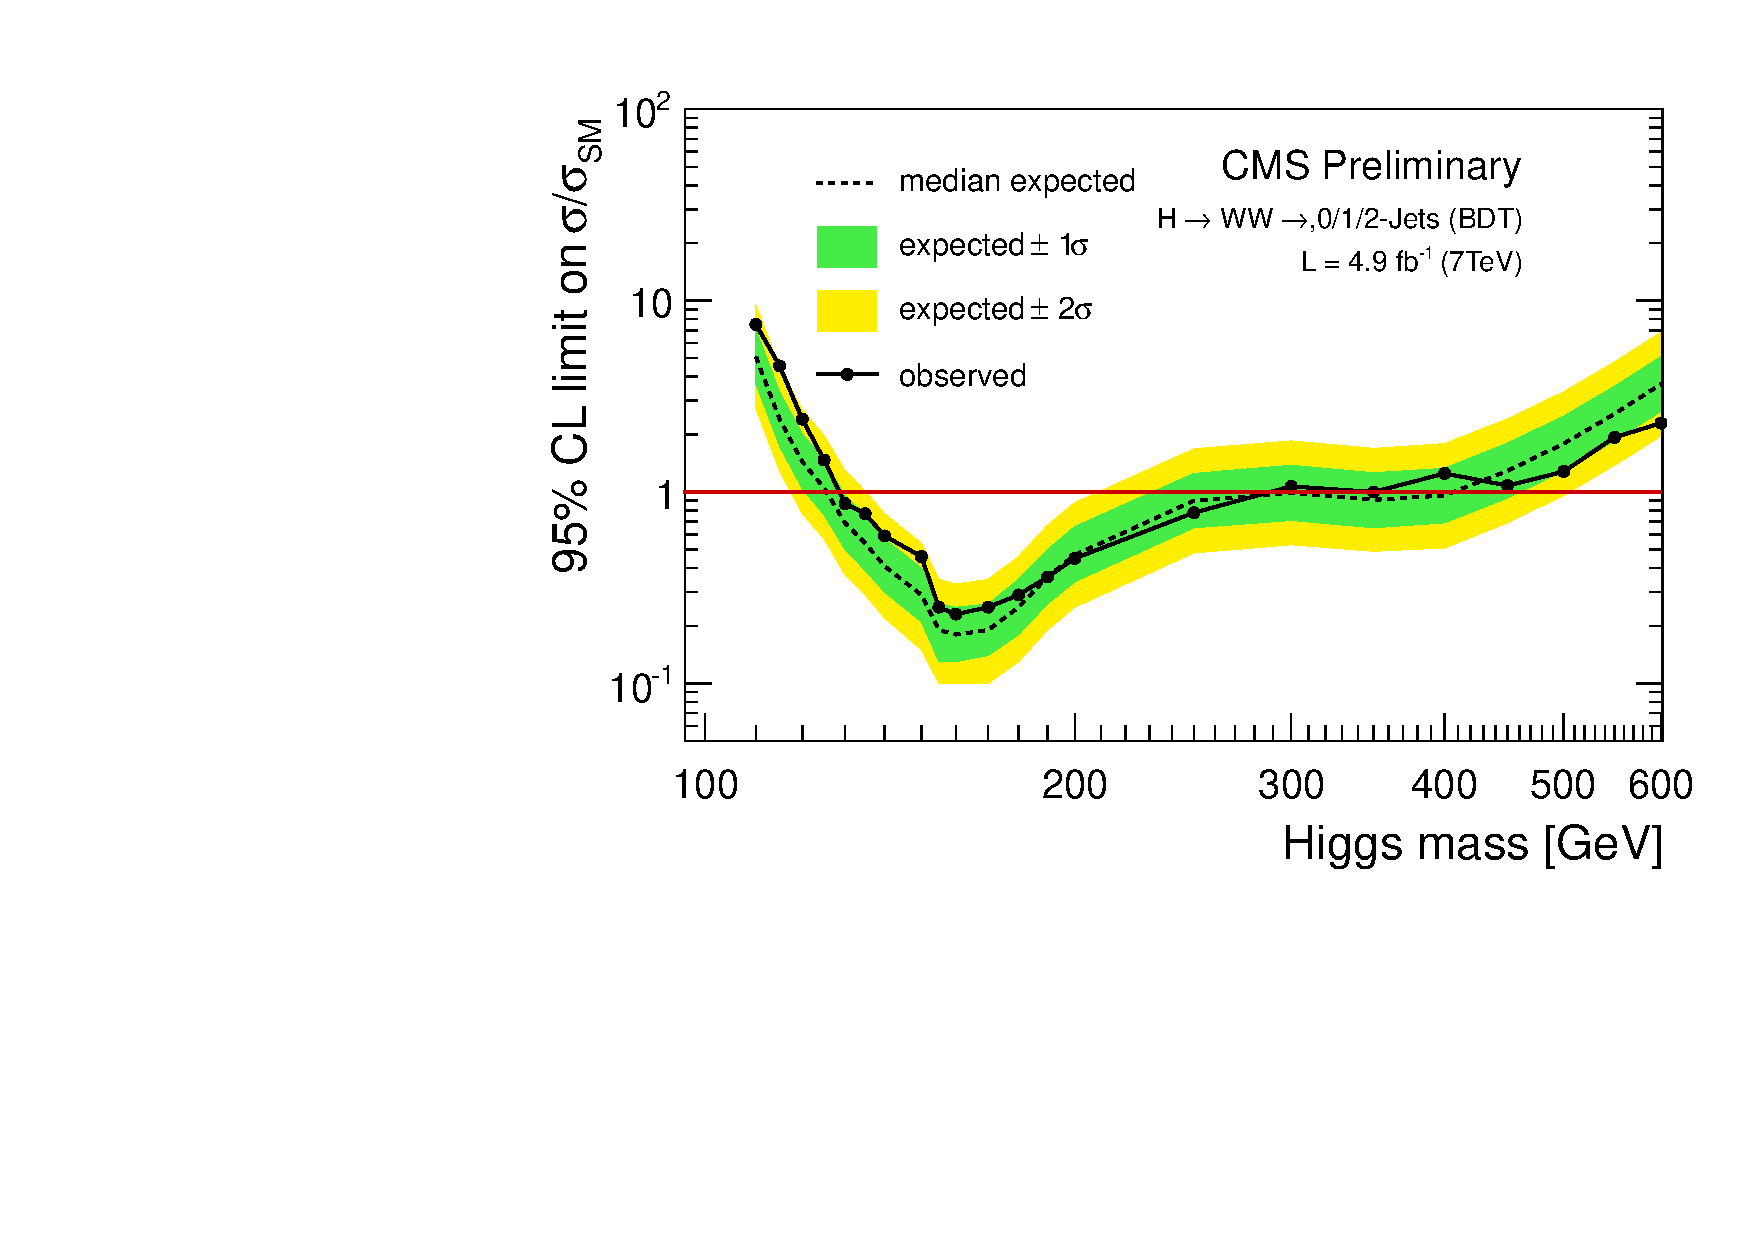
\includegraphics[width=.45\textwidth]{figures/limits_nj_shape_7TeV-CLs-asymptotic_log.pdf}}
\centering
\subfigure[SM Higgs (shape-based) 8 TeV ]{
\centering
\label{subfig:sm_shape_8tev}
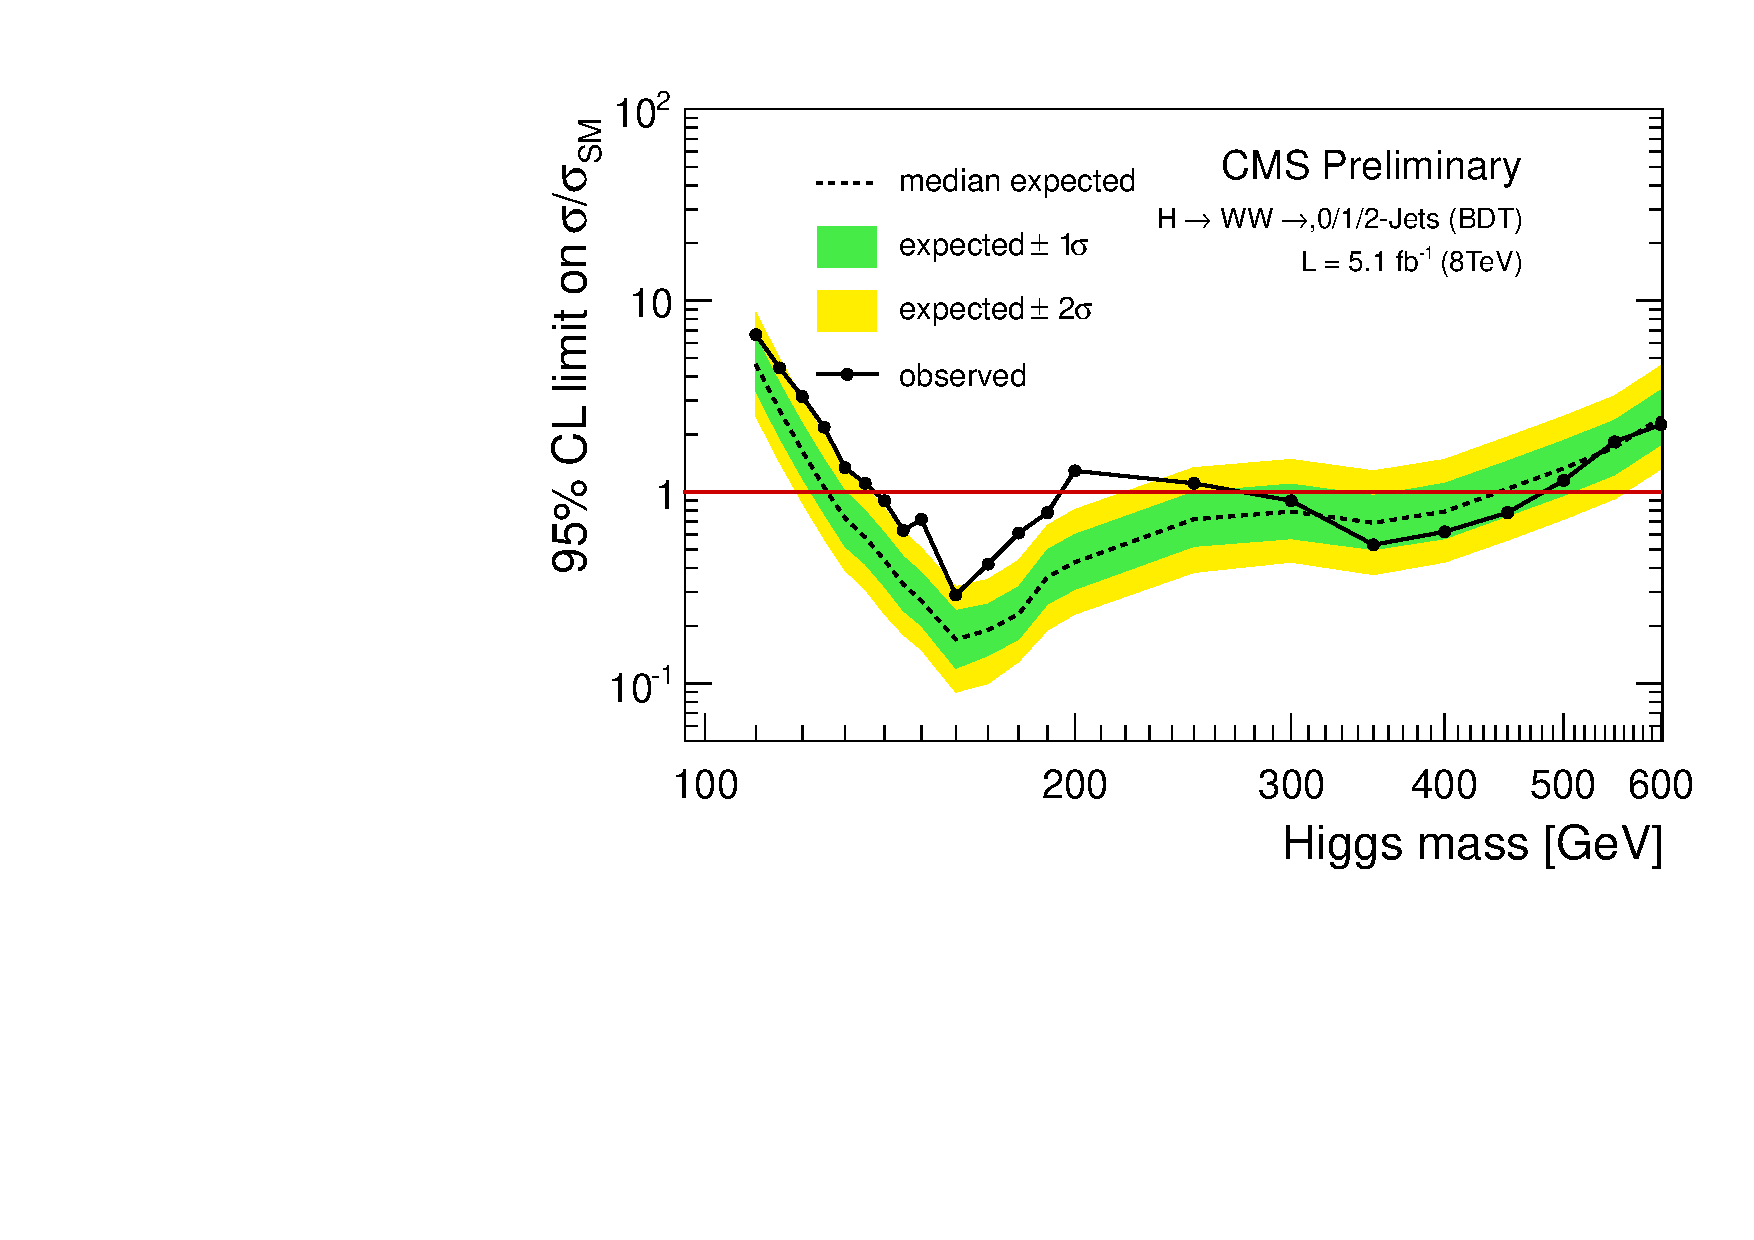
\includegraphics[width=.45\textwidth]{figures/limits_nj_shape_8TeV-CLs-asymptotic_log.pdf}} \\
\subfigure[SM Higgs (shape-based) 7+8 TeV ]{
\centering
\label{subfig:sm_shape_comb}
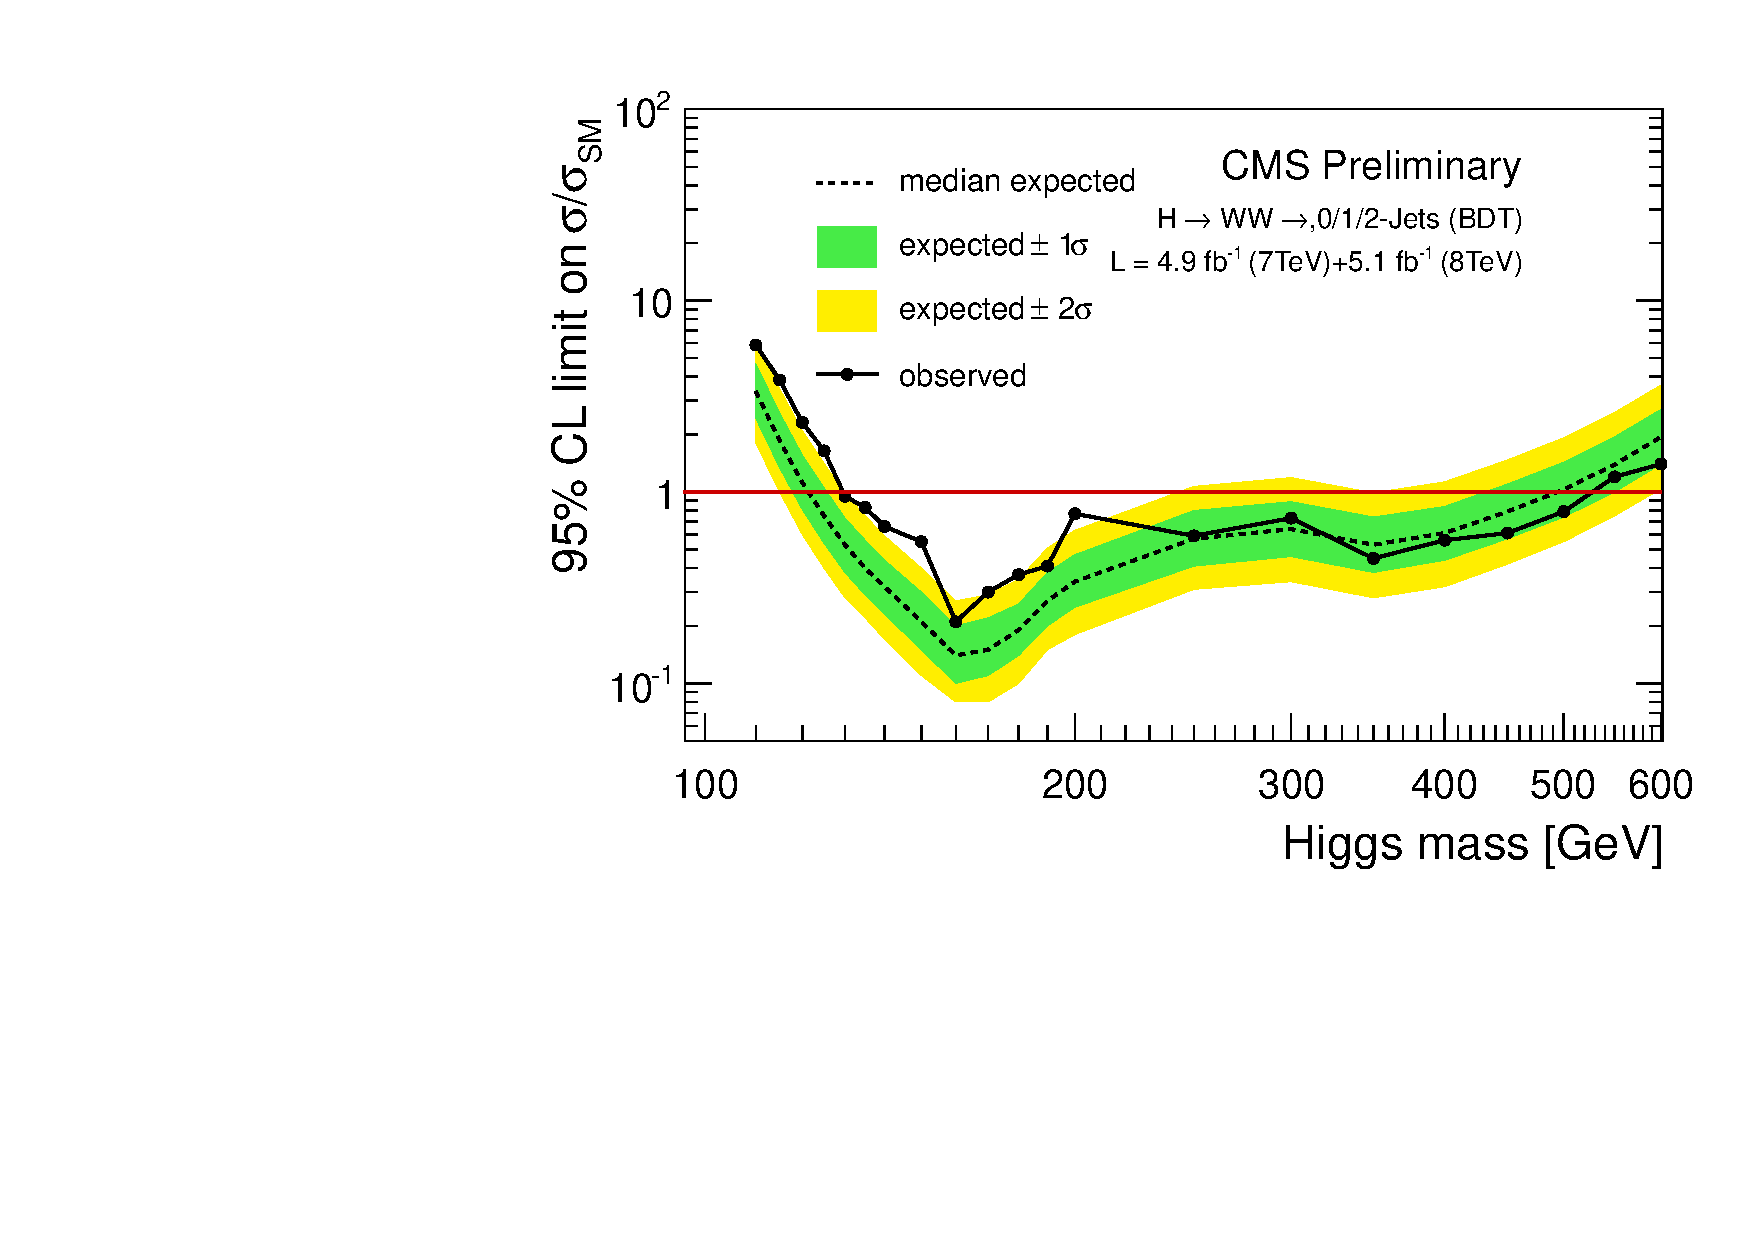
\includegraphics[width=.45\textwidth]{figures/limits_nj_shape-CLs-asymptotic_log.pdf}} \\ 
\label{fig:uls_shape}
\caption{Expected and observed upper limits for SM Higgs using the
  {\bf shape-based} analysis using 7 TeV, 8 TeV and combined data.}
\end{figure}

%%%%%%%%%%%%%%%%%%%%%%%%%%%%%%%%%%%%%%%%%%%%%%%%%%%%%%%%%%%%
\begin{table}[hbp!]
\begin{center}
\begin{tabular}{c c c c c}
\hline
\vspace{-3mm} && \\
 Higgs Mass & Observed  & Median expected & Expected range for 68\% & Expected range for 95\%   \\
\hline
\vspace{-3mm} && \\
110 & 7.51 & 5.09 & [3.67, 7.08] & [2.73, 9.49] \\
115 & 4.56 & 2.40 & [1.73, 3.33] & [1.29, 4.47] \\
120 & 2.40 & 1.44 & [1.04, 2.01] & [0.77, 2.69] \\
125 & 1.47 & 1.05 & [0.76, 1.47] & [0.57, 1.97] \\
130 & 0.87 & 0.69 & [0.50, 0.96] & [0.37, 1.29] \\
135 & 0.77 & 0.54 & [0.39, 0.76] & [0.29, 1.01] \\
140 & 0.59 & 0.41 & [0.30, 0.57] & [0.22, 0.77] \\
150 & 0.14 & 0.29 & [0.21, 0.40] & [0.15, 0.54] \\
160 & 0.23 & 0.18 & [0.13, 0.25] & [0.10, 0.33] \\
170 & 0.25 & 0.19 & [0.14, 0.26] & [0.10, 0.35] \\
180 & 0.29 & 0.25 & [0.18, 0.35] & [0.13, 0.46] \\
190 & 0.36 & 0.36 & [0.26, 0.50] & [0.19, 0.67] \\
200 & 0.45 & 0.47 & [0.34, 0.66] & [0.25, 0.88] \\
250 & 0.78 & 0.90 & [0.65, 1.25] & [0.48, 1.68] \\
300 & 1.07 & 0.99 & [0.71, 1.38] & [0.53, 1.85] \\
350 & 1.00 & 0.91 & [0.65, 1.26] & [0.49, 1.69] \\
400 & 1.25 & 0.96 & [0.69, 1.33] & [0.51, 1.79] \\
450 & 1.08 & 1.29 & [0.93, 1.80] & [0.69, 2.41] \\
500 & 1.28 & 1.79 & [1.29, 2.49] & [0.96, 3.34] \\
550 & 1.93 & 2.56 & [1.85, 3.57] & [1.38, 4.78] \\
600 & 2.29 & 3.66 & [2.64, 5.09] & [1.96, 6.83] \\
\hline
\end{tabular}
\caption{Expected and observed upper limits for SM Higgs using the
  {\bf shape-based} analysis, corresponding to $\intlumiSevenTeV$ at 7 TeV. }
\label{tab:shapebase_uls_7tev}
\end{center}
%\end{table}
%%%%%%%%%%%%%%%%%%%%%%%%%%%%%%
%\begin{table}[hbp!]
\begin{center}
\begin{tabular}{c c c c c}
\hline
\vspace{-3mm} && \\
 Higgs Mass & Observed  & Median expected & Expected range for 68\% & Expected range for 95\%   \\
\vspace{-3mm} && \\
\hline
110 & 6.64 & 4.64 & [3.34, 6.45] & [2.49, 8.65] \\
115 & 4.45 & 2.67 & [1.92, 3.71] & [1.43, 4.98] \\
120 & 3.15 & 1.64 & [1.18, 2.28] & [0.88, 3.06] \\
125 & 2.18 & 1.06 & [0.77, 1.48] & [0.57, 1.99] \\
130 & 1.34 & 0.73 & [0.52, 1.01] & [0.39, 1.35] \\
135 & 1.11 & 0.58 & [0.42, 0.80] & [0.31, 1.08] \\
140 & 0.90 & 0.44 & [0.32, 0.61] & [0.23, 0.82] \\
145 & 0.63 & 0.33 & [0.24, 0.46] & [0.18, 0.62] \\
150 & 0.72 & 0.27 & [0.20, 0.38] & [0.15, 0.51] \\
160 & 0.29 & 0.17 & [0.12, 0.24] & [0.09, 0.32] \\
170 & 0.42 & 0.19 & [0.14, 0.26] & [0.10, 0.35] \\
180 & 0.61 & 0.23 & [0.17, 0.32] & [0.13, 0.44] \\
190 & 0.78 & 0.36 & [0.26, 0.50] & [0.19, 0.67] \\
200 & 1.29 & 0.43 & [0.31, 0.60] & [0.23, 0.81] \\
% 200 & 0.34 & 0.43 & [0.31, 0.60] & [0.23, 0.81] \\ rMax = 50 for observed
250 & 1.11 & 0.72 & [0.52, 1.00] & [0.38, 1.34] \\
300 & 0.90 & 0.79 & [0.57, 1.10] & [0.43, 1.48] \\
350 & 0.53 & 0.69 & [0.50, 0.96] & [0.37, 1.29] \\
400 & 0.62 & 0.79 & [0.57, 1.11] & [0.43, 1.48] \\
450 & 0.78 & 1.04 & [0.75, 1.45] & [0.56, 1.94] \\
500 & 1.15 & 1.33 & [0.96, 1.86] & [0.72, 2.49] \\
550 & 1.83 & 1.71 & [1.23, 2.37] & [0.92, 3.18] \\
600 & 2.25 & 2.45 & [1.77, 3.41] & [1.32, 4.57] \\
\hline
\end{tabular}
\caption{Expected and observed upper limits for SM Higgs using the
  {\bf shape-based} analysis with \intlumiEightTeV\ of data at 8 TeV.}
\label{tab:shapebase_uls_8tev}
\end{center}
\end{table}
%%%%%%%%%%%%%%%%%%%%%%%%%%%%%%
\begin{table}[hbp!]
\begin{center}
\begin{tabular}{c c c c c}
\hline
\vspace{-3mm} && \\
 Higgs Mass & Observed  & Median expected & Expected range for 68\% & Expected range for 95\%   \\
\hline
110 & 5.86 & 3.35 & [2.42, 4.67] & [1.80, 6.25] \\
115 & 3.85 & 1.86 & [1.34, 2.59] & [1.00, 3.47] \\
120 & 2.31 & 1.12 & [0.81, 1.56] & [0.60, 2.09] \\
125 & 1.64 & 0.75 & [0.54, 1.05] & [0.40, 1.41] \\
130 & 0.95 & 0.53 & [0.38, 0.73] & [0.28, 0.98] \\
135 & 0.83 & 0.40 & [0.29, 0.56] & [0.22, 0.75] \\
140 & 0.66 & 0.32 & [0.23, 0.44] & [0.17, 0.59] \\
150 & 0.55 & 0.21 & [0.15, 0.30] & [0.11, 0.40] \\
160 & 0.21 & 0.14 & [0.10, 0.20] & [0.08, 0.27] \\
170 & 0.30 & 0.15 & [0.11, 0.22] & [0.08, 0.29] \\
180 & 0.37 & 0.19 & [0.14, 0.26] & [0.10, 0.35] \\
190 & 0.41 & 0.27 & [0.20, 0.38] & [0.15, 0.51] \\
200 & 0.77 & 0.34 & [0.25, 0.47] & [0.18, 0.63] \\
250 & 0.59 & 0.57 & [0.41, 0.80] & [0.31, 1.07] \\
300 & 0.73 & 0.64 & [0.46, 0.89] & [0.34, 1.19] \\
350 & 0.45 & 0.53 & [0.38, 0.74] & [0.28, 0.99] \\
400 & 0.56 & 0.61 & [0.44, 0.84] & [0.32, 1.13] \\
450 & 0.61 & 0.79 & [0.57, 1.10] & [0.42, 1.47] \\
500 & 0.79 & 1.03 & [0.74, 1.43] & [0.55, 1.92] \\
550 & 1.20 & 1.39 & [1.00, 1.94] & [0.75, 2.60] \\
600 & 1.40 & 1.94 & [1.40, 2.70] & [1.04, 3.62] \\
\hline
\end{tabular}
\caption{Expected and observed upper limits for SM Higgs using the
  {\bf shape-based} analysis, corresponding to $\intlumiSevenTeV$ at 7 TeV and $\intlumiEightTeV$ 8 TeV data.}
\label{tab:shapebase_uls_7and8tev}
\end{center}
\end{table}
%%%%%%%%%%%%%%%%%%%%%%%%%%%%%
\clearpage


\subsection{Detailed Results at 8 TeV}

%%%%%%%%%%%%%%%%%%%%%%%%%%%%%%
\begin{figure}[!hbtp]
\centering
\subfigure[SM Higgs (shape-based) 8 TeV 0-Jet OF ]{
\centering
\label{subfig:sm_shape_8tev_0jof}
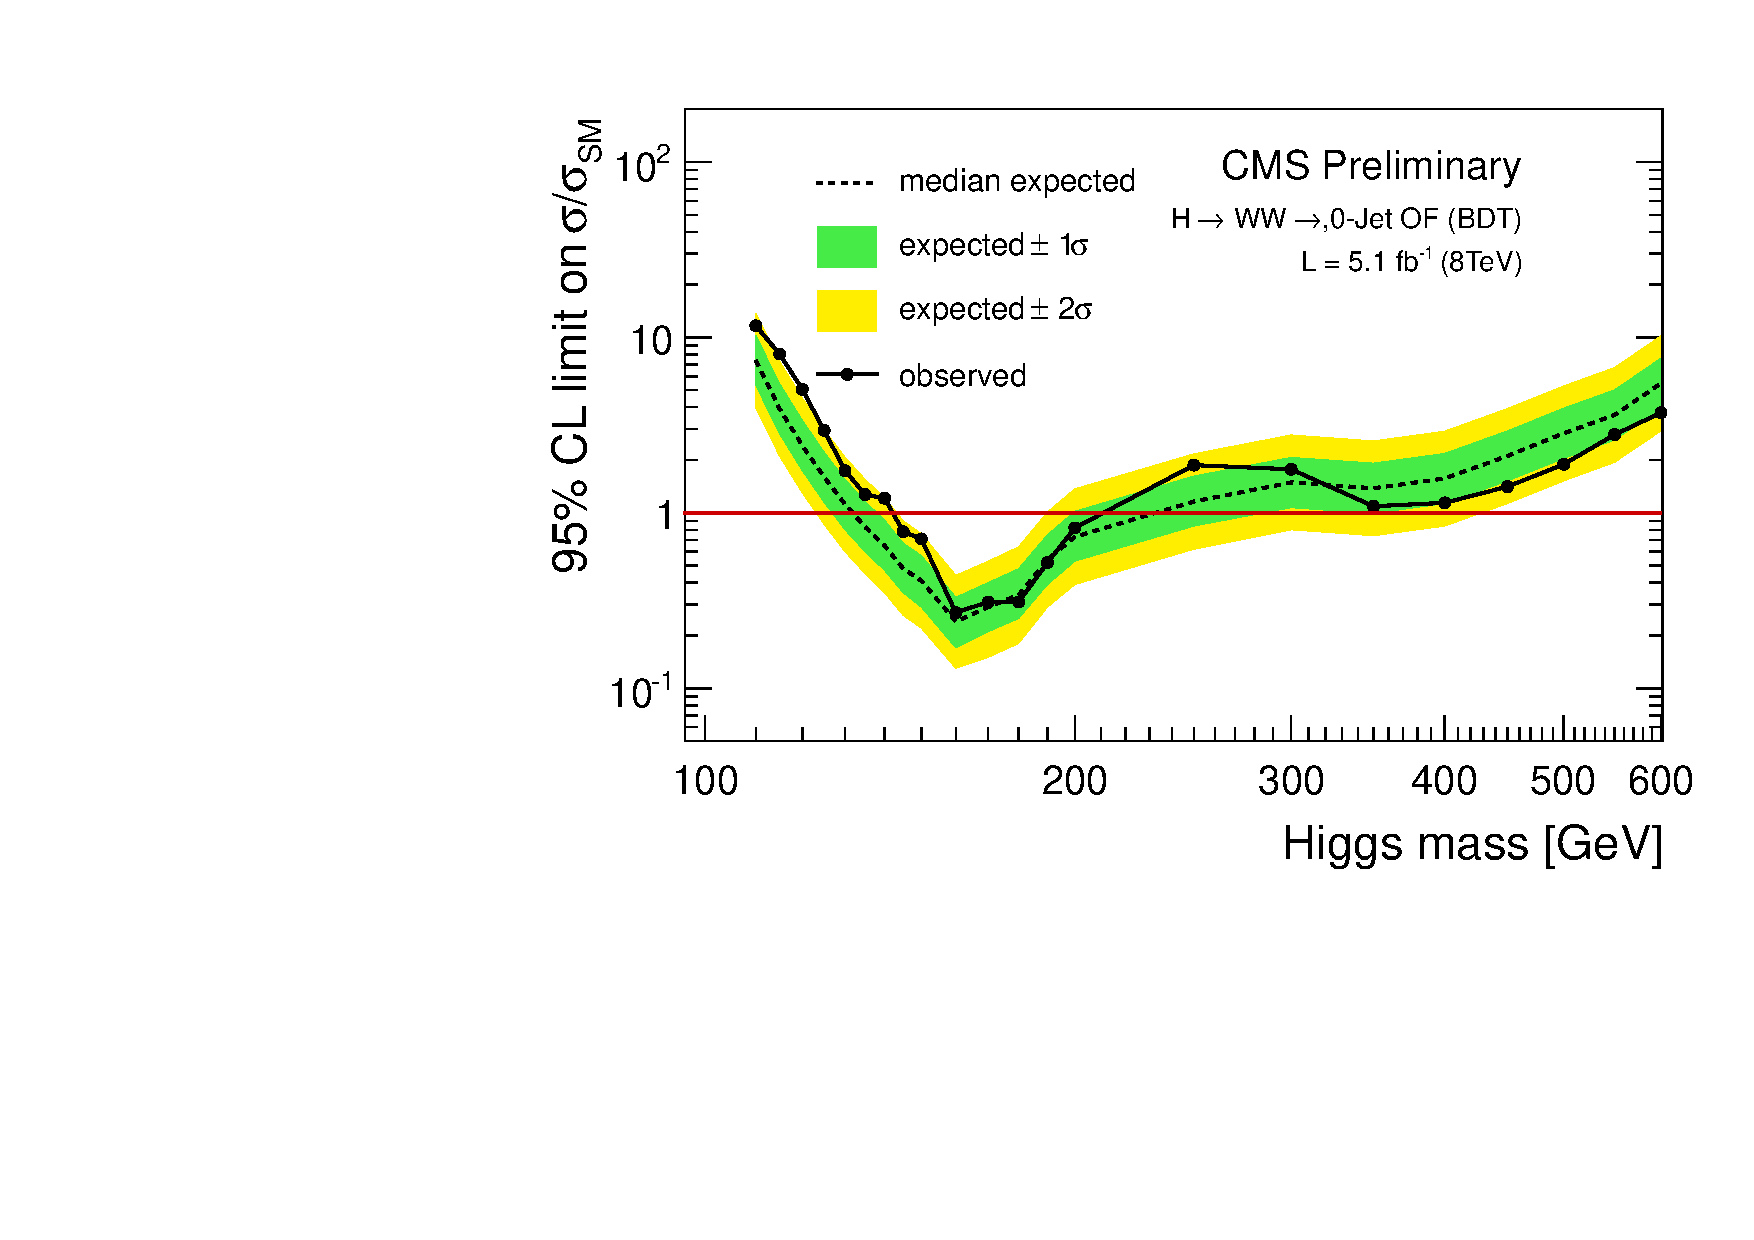
\includegraphics[width=.45\textwidth]{figures/limits_0jof_shape_8TeV-CLs-asymptotic_log.pdf}}
\subfigure[SM Higgs (shape-based) 8 TeV 0-Jet SF ]{
\centering
\label{subfig:sm_shape_8tev_0jsf}
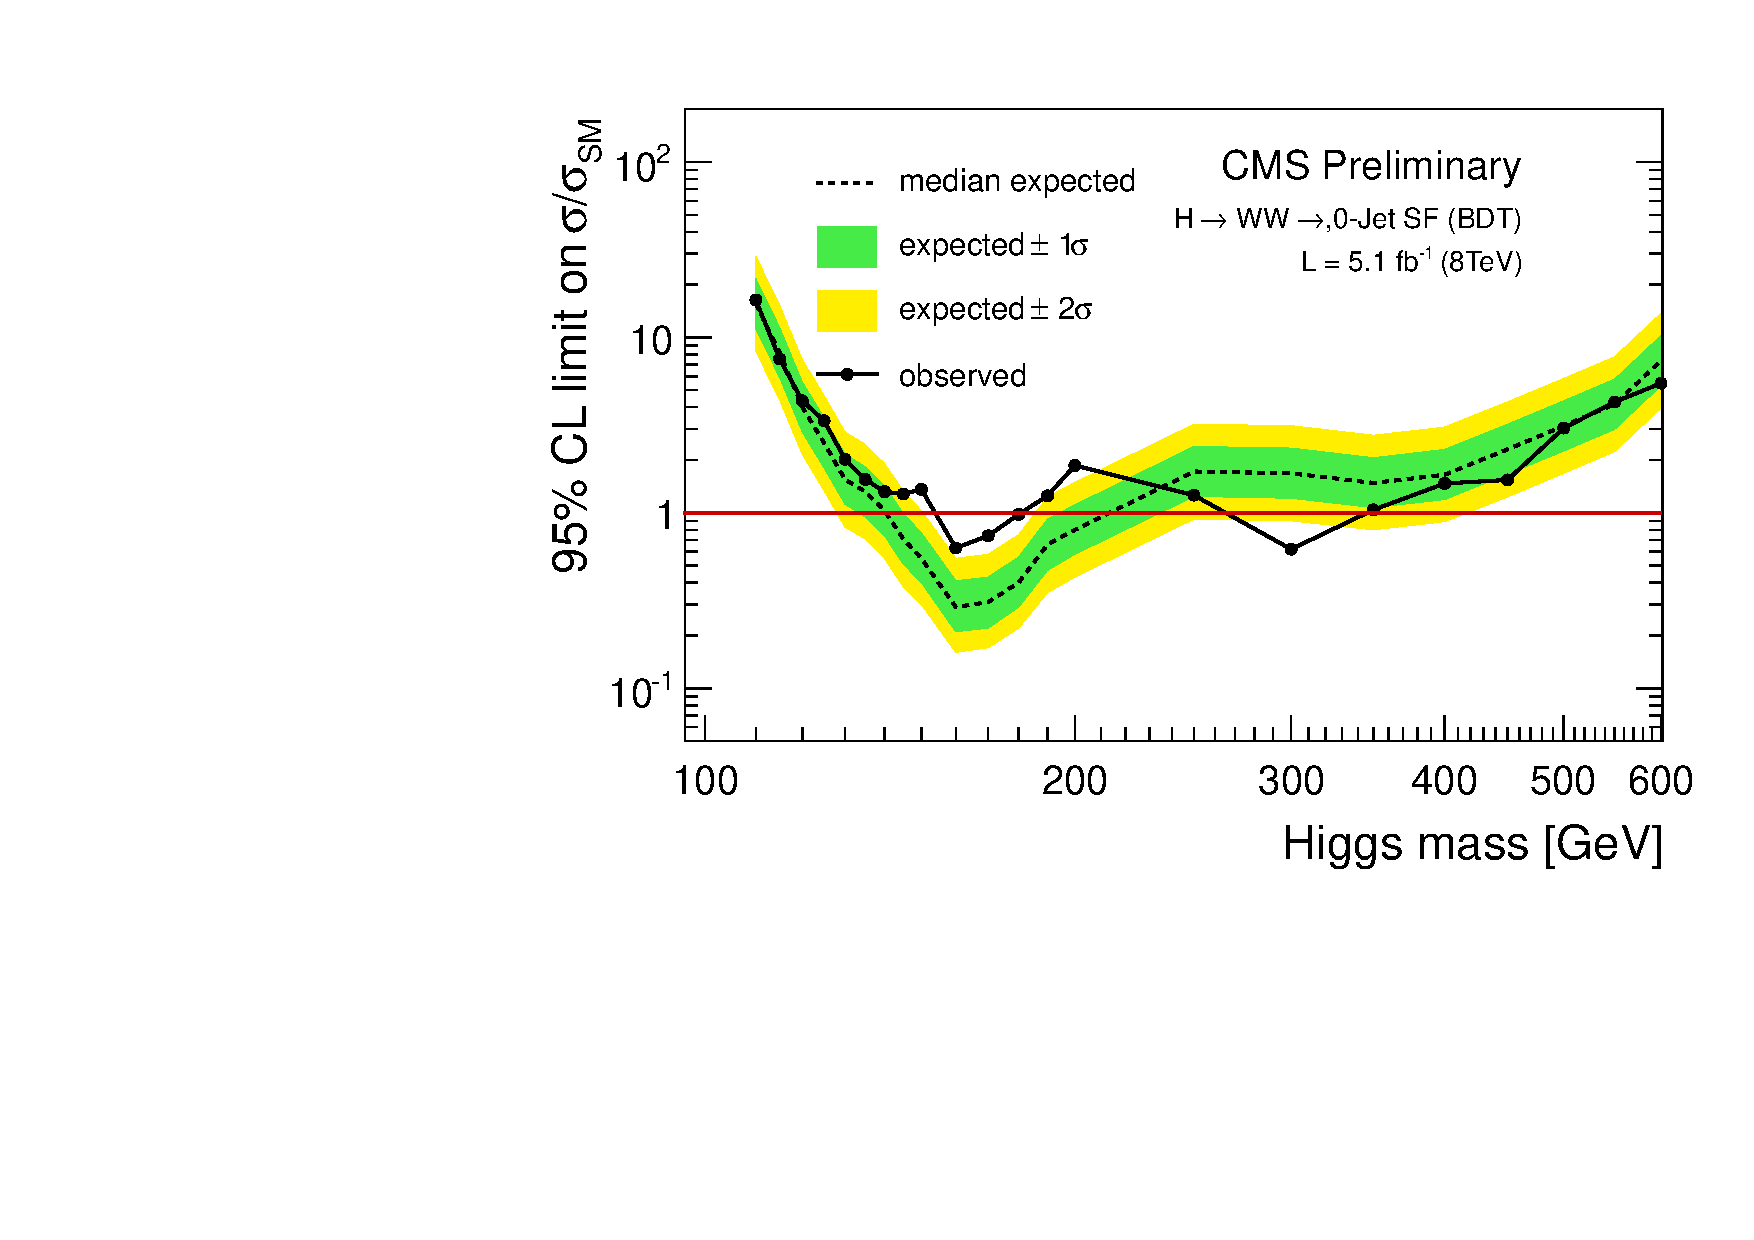
\includegraphics[width=.45\textwidth]{figures/limits_0jsf_shape_8TeV-CLs-asymptotic_log.pdf}} \\
\subfigure[SM Higgs (shape-based) 8 TeV 1-Jet OF ]{
\centering
\label{subfig:sm_shape_8tev_1jof}
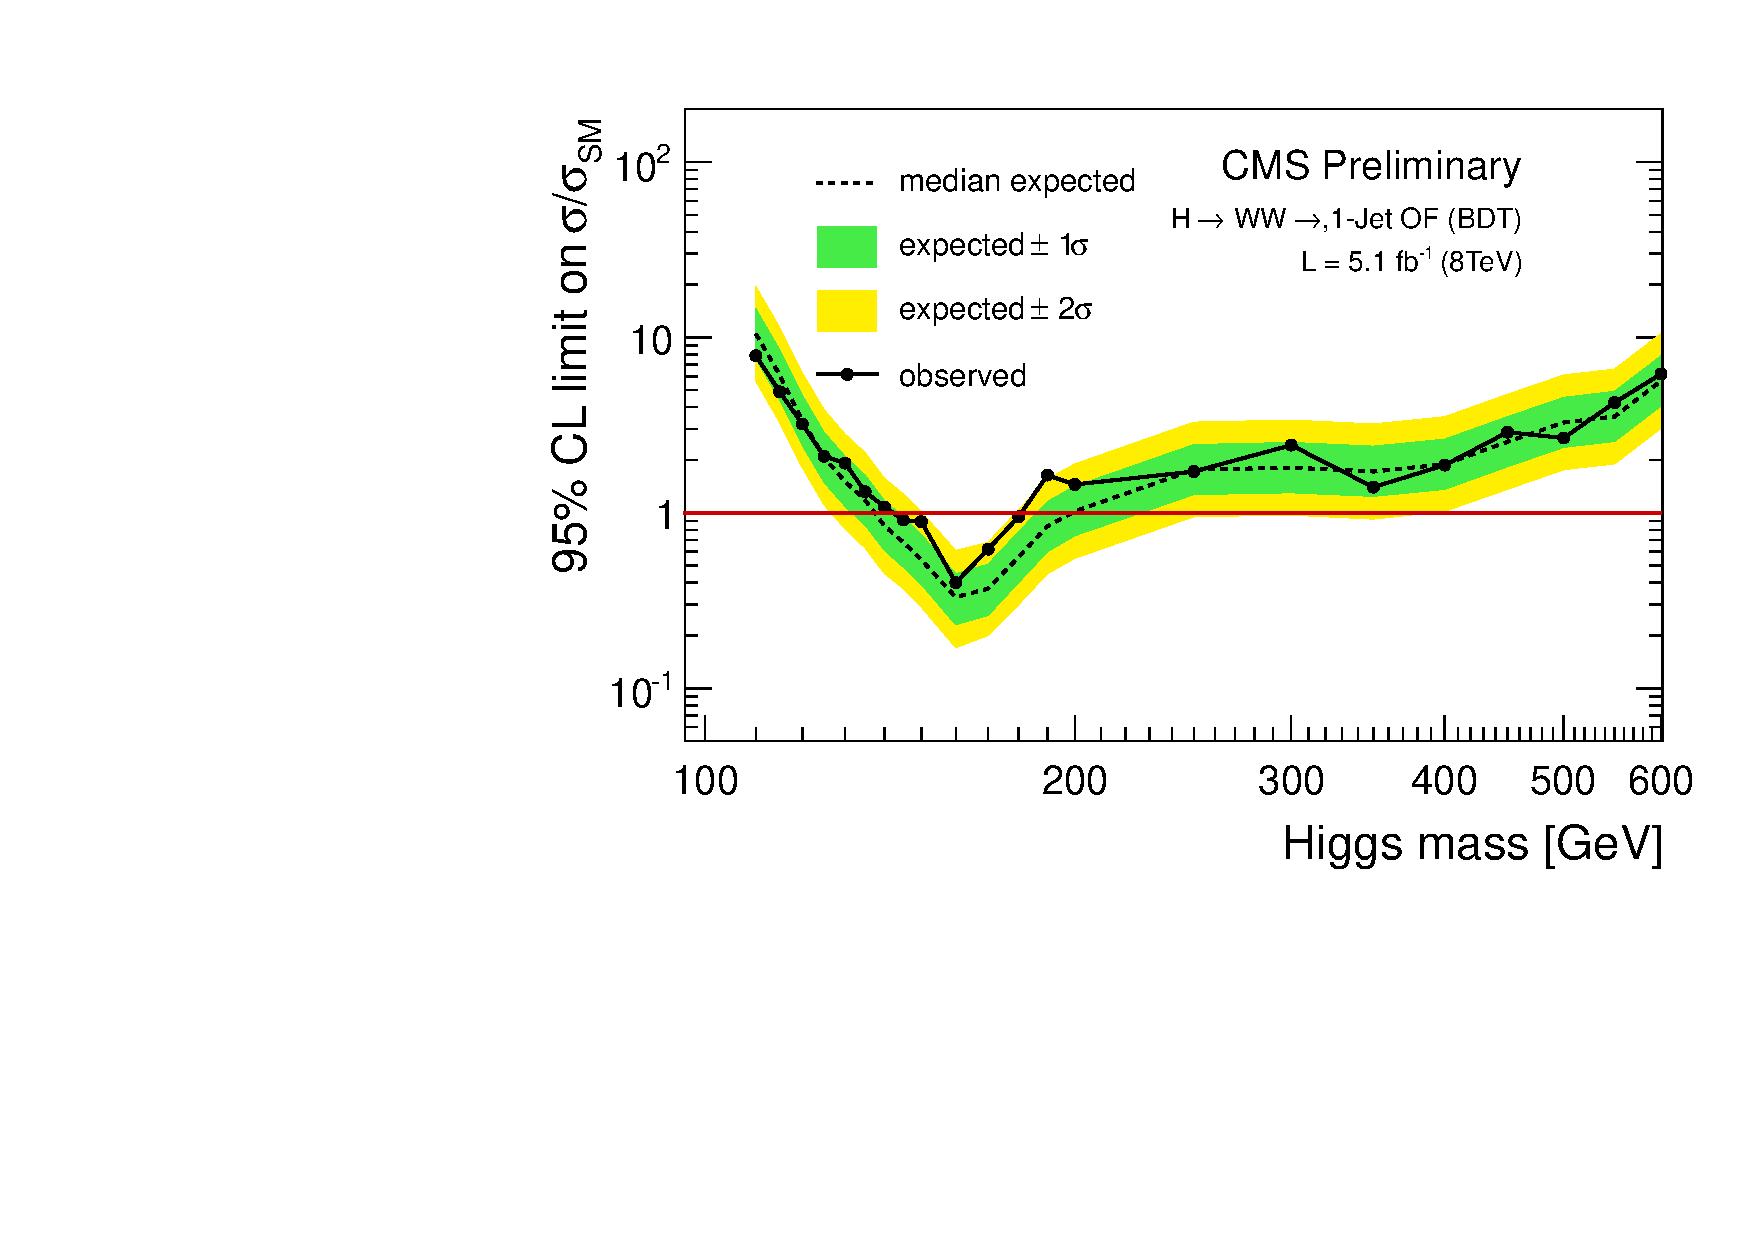
\includegraphics[width=.45\textwidth]{figures/limits_1jof_shape_8TeV-CLs-asymptotic_log.pdf}}
\subfigure[SM Higgs (shape-based) 8 TeV 1-Jet SF ]{
\centering
\label{subfig:sm_shape_8tev_1jsf}
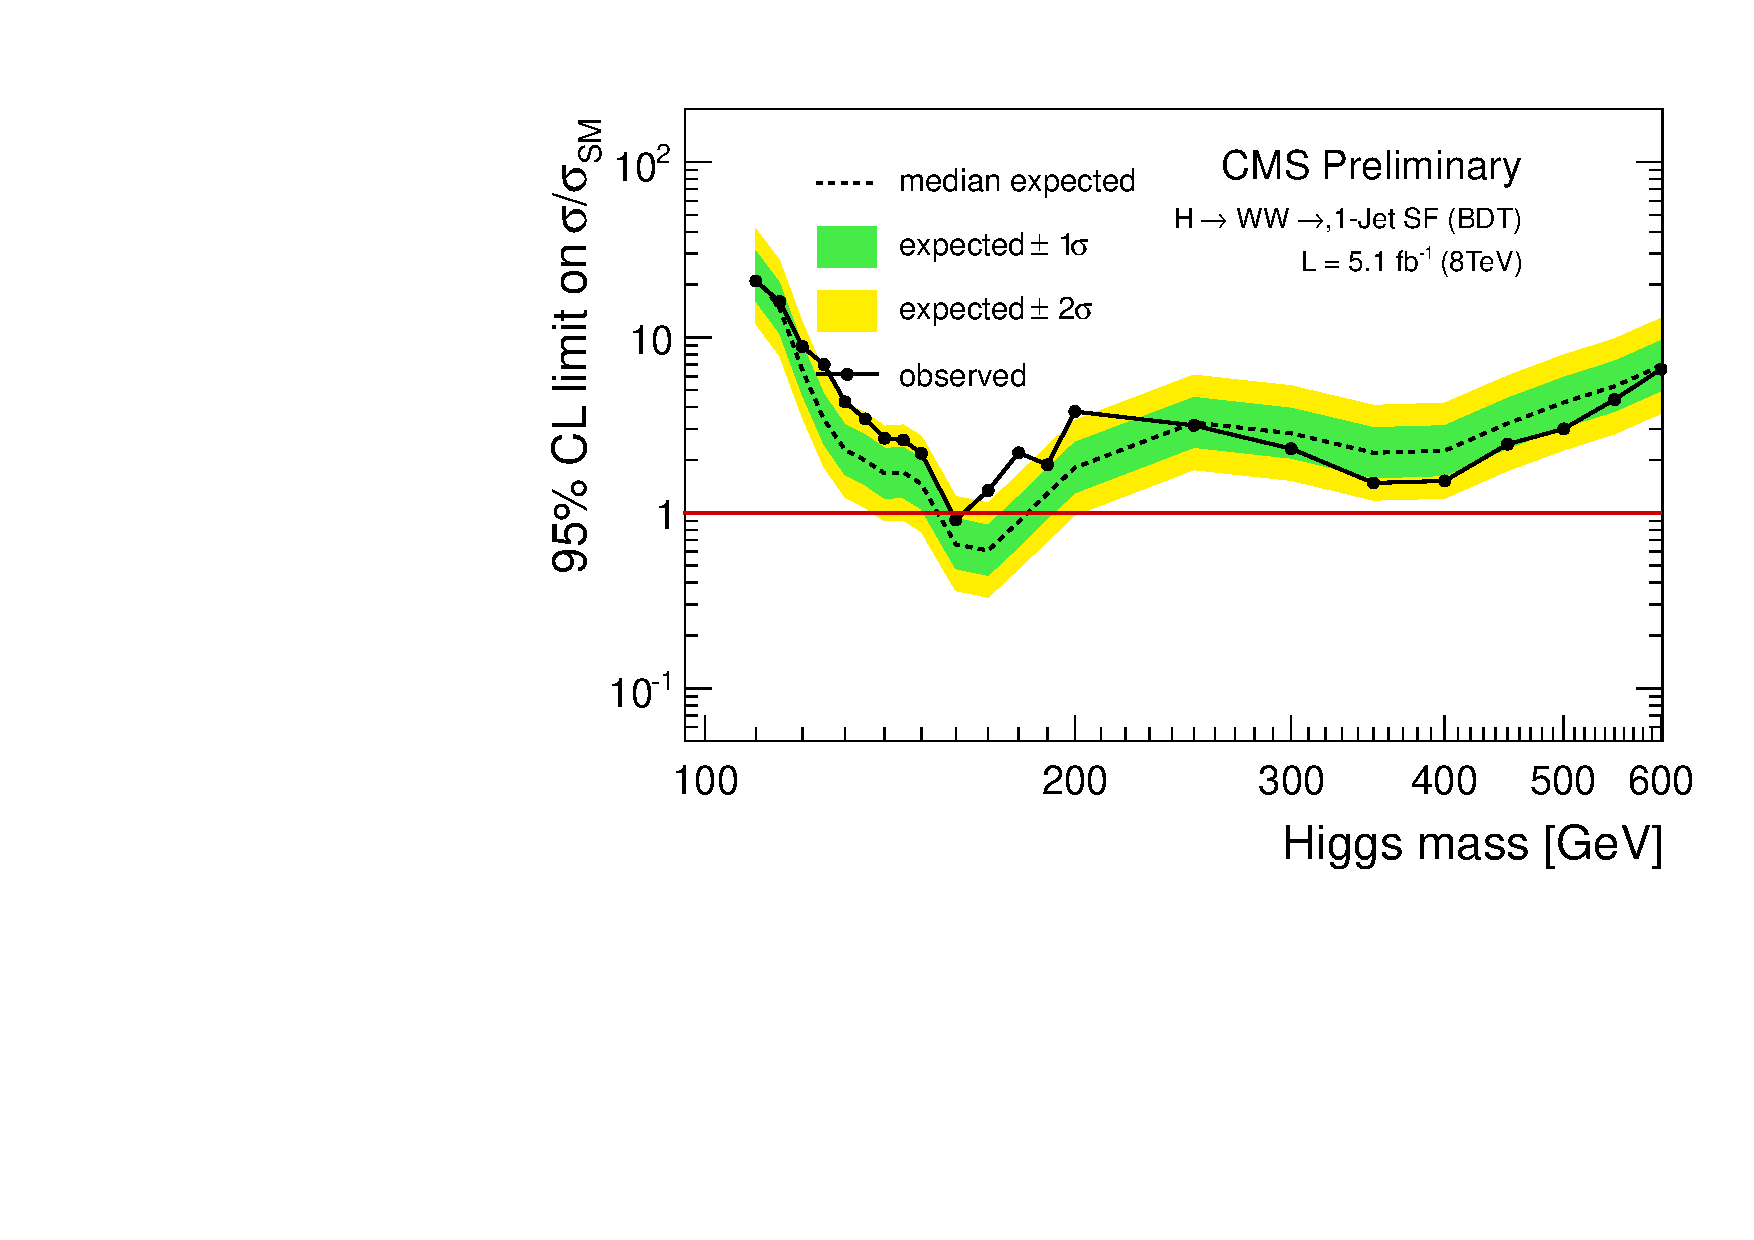
\includegraphics[width=.45\textwidth]{figures/limits_1jsf_shape_8TeV-CLs-asymptotic_log.pdf}} \\
\label{fig:uls_shape_8tev}
\caption{Expected and observed upper limits for SM Higgs using the
  {\bf shape-based} analysis using {\bf 8 TeV data}.}
\end{figure}
%%%%%%%%%%%%%%%%%%%%%%%%%%%%%%%%%%%%%%%%%%%%%%%%%%%%%%%%%%%%
%%%%%%%%%%%%%%%%%%%%%%%%%%%%%%
\begin{table}[hbp!]
\begin{center}
\begin{tabular}{c c c c c}
\hline
\vspace{-3mm} && \\
 Higgs Mass & Observed  & Median expected & Expected range for 68\% & Expected range for 95\%   \\
\vspace{-3mm} && \\
\hline
\multicolumn{5}{c}{0-Jet OF} \\
\hline
110 & 11.65 & 7.38 & [5.32, 10.27] & [3.96, 13.77] \\
115 & 8.04 & 3.92 & [2.82, 5.45] & [2.10, 7.31] \\
120 & 5.06 & 2.42 & [1.74, 3.37] & [1.30, 4.51] \\
125 & 2.95 & 1.60 & [1.15, 2.22] & [0.86, 2.98] \\
130 & 1.74 & 1.12 & [0.80, 1.55] & [0.60, 2.08] \\
135 & 1.27 & 0.83 & [0.60, 1.16] & [0.45, 1.55] \\
140 & 1.21 & 0.65 & [0.47, 0.91] & [0.35, 1.22] \\
145 & 0.78 & 0.48 & [0.35, 0.67] & [0.26, 0.90] \\
150 & 0.71 & 0.41 & [0.29, 0.57] & [0.22, 0.76] \\
160 & 0.27 & 0.24 & [0.17, 0.33] & [0.13, 0.44] \\
170 & 0.31 & 0.29 & [0.21, 0.40] & [0.15, 0.53] \\
180 & 0.31 & 0.34 & [0.25, 0.48] & [0.18, 0.64] \\
190 & 0.52 & 0.54 & [0.39, 0.75] & [0.29, 1.01] \\
200 & 0.82 & 0.73 & [0.53, 1.02] & [0.39, 1.37] \\
250 & 1.87 & 1.16 & [0.84, 1.62] & [0.62, 2.17] \\
300 & 1.77 & 1.49 & [1.07, 2.07] & [0.80, 2.78] \\
350 & 1.09 & 1.38 & [0.99, 1.92] & [0.74, 2.57] \\
400 & 1.14 & 1.57 & [1.13, 2.18] & [0.84, 2.92] \\
450 & 1.41 & 2.11 & [1.52, 2.93] & [1.13, 3.93] \\
500 & 1.89 & 2.84 & [2.04, 3.95] & [1.52, 5.29] \\
550 & 2.79 & 3.61 & [2.60, 5.02] & [1.94, 6.73] \\
600 & 3.72 & 5.47 & [3.94, 7.61] & [2.93, 10.20] \\
\hline
\multicolumn{5}{c}{0-Jet SF} \\
\hline
110 & 16.34 & 15.52 & [11.18, 21.60] & [8.33, 28.96] \\
115 & 7.54 & 8.20 & [5.91, 11.41] & [4.40, 15.30] \\
120 & 4.35 & 4.01 & [2.89, 5.57] & [2.15, 7.47] \\
125 & 3.35 & 2.50 & [1.80, 3.48] & [1.34, 4.66] \\
130 & 2.02 & 1.55 & [1.12, 2.16] & [0.83, 2.89] \\
135 & 1.55 & 1.32 & [0.95, 1.83] & [0.71, 2.46] \\
140 & 1.32 & 1.03 & [0.74, 1.43] & [0.55, 1.91] \\
145 & 1.28 & 0.71 & [0.51, 0.99] & [0.38, 1.33] \\
150 & 1.36 & 0.55 & [0.40, 0.77] & [0.30, 1.03] \\
160 & 0.63 & 0.29 & [0.21, 0.41] & [0.16, 0.55] \\
170 & 0.74 & 0.31 & [0.22, 0.43] & [0.17, 0.58] \\
180 & 0.98 & 0.40 & [0.29, 0.56] & [0.22, 0.75] \\
190 & 1.25 & 0.66 & [0.47, 0.92] & [0.35, 1.23] \\
200 & 1.86 & 0.80 & [0.58, 1.11] & [0.43, 1.49] \\
250 & 1.26 & 1.72 & [1.24, 2.39] & [0.92, 3.20] \\
% 250 & 1.26 & 19.93 & [14.36, 27.73] & [10.69, 37.18] \\ rMax = 30 for exp
300 & 0.62 & 1.68 & [1.21, 2.34] & [0.90, 3.14] \\
350 & 1.04 & 1.48 & [1.07, 2.06] & [0.80, 2.77] \\
400 & 1.47 & 1.65 & [1.19, 2.30] & [0.89, 3.08] \\
% 400 & 1.47 & 18.95 & [13.65, 26.37] & [10.17, 35.35] \\ rMax = 30 for exp
450 & 1.54 & 2.30 & [1.66, 3.20] & [1.23, 4.29] \\
500 & 3.04 & 3.13 & [2.25, 4.35] & [1.68, 5.83] \\
550 & 4.28 & 4.16 & [2.99, 5.78] & [2.23, 7.75] \\
600 & 5.48 & 7.36 & [5.30, 10.24] & [3.95, 13.73] \\

\hline
\end{tabular}
\caption{Expected and observed upper limits for SM Higgs using the
  {\bf shape-based} analysis with \intlumiEightTeV\ of data in the {\bf 0-Jet} final state.}
\label{tab:shapebase_uls_0j}
\end{center}
\end{table}
%%%%%%%%%%%%%%%%%%%%%%%%%%%%%%

%%%%%%%%%%%%%%%%%%%%%%%%%%%%%%%%%%%%%%%%%%%%%%%%%%%%%%%%%%%%
%%%%%%%%%%%%%%%%%%%%%%%%%%%%%%
\begin{table}[hbp!]
\begin{center}
\begin{tabular}{c c c c c  }
\hline
\vspace{-3mm} && \\
 Higgs Mass & Observed  & Median expected & Expected range for 68\% & Expected range for 95\%   \\
\vspace{-3mm} && \\
\hline
\multicolumn{5}{c}{1-Jet OF} \\
\hline
110 & 7.86 & 10.47 & [7.54, 14.56] & [5.62, 19.52] \\
115 & 4.90 & 6.12 & [4.41, 8.51] & [3.28, 11.41] \\
120 & 3.21 & 3.37 & [2.42, 4.68] & [1.81, 6.28] \\
125 & 2.10 & 2.07 & [1.49, 2.88] & [1.11, 3.87] \\
130 & 1.92 & 1.51 & [1.09, 2.10] & [0.81, 2.81] \\
135 & 1.32 & 1.18 & [0.85, 1.64] & [0.63, 2.20] \\
140 & 1.08 & 0.84 & [0.61, 1.17] & [0.45, 1.57] \\
145 & 0.91 & 0.68 & [0.49, 0.95] & [0.37, 1.28] \\
150 & 0.89 & 0.54 & [0.39, 0.75] & [0.29, 1.01] \\
160 & 0.40 & 0.33 & [0.23, 0.45] & [0.17, 0.61] \\
170 & 0.62 & 0.37 & [0.26, 0.51] & [0.20, 0.68] \\
180 & 0.95 & 0.56 & [0.40, 0.78] & [0.30, 1.04] \\
190 & 1.64 & 0.84 & [0.60, 1.16] & [0.45, 1.56] \\
200 & 1.45 & 1.02 & [0.74, 1.42] & [0.55, 1.90] \\
250 & 1.72 & 1.76 & [1.27, 2.45] & [0.95, 3.29] \\
300 & 2.43 & 1.81 & [1.30, 2.52] & [0.97, 3.38] \\
350 & 1.40 & 1.72 & [1.24, 2.40] & [0.92, 3.21] \\
400 & 1.87 & 1.89 & [1.36, 2.63] & [1.02, 3.53] \\
%350 & 1.40 & 19.73 & [14.21, 27.45] & [10.59, 36.80] \\ rMax = 30 for exp
%400 & 1.87 & 20.45 & [14.73, 28.46] & [10.97, 38.15] \\ rMax = 30 for exp
450 & 2.88 & 2.54 & [1.83, 3.53] & [1.36, 4.74] \\
500 & 2.67 & 3.27 & [2.36, 4.55] & [1.76, 6.11] \\
550 & 4.25 & 3.54 & [2.55, 4.93] & [1.90, 6.60] \\
600 & 6.18 & 5.64 & [4.06, 7.85] & [3.03, 10.52] \\
\hline
\multicolumn{5}{c}{1-Jet SF} \\
\hline
110 & 20.96 & 22.26 & [16.04, 30.98] & [11.95, 41.53] \\
115 & 16.00 & 14.67 & [10.57, 20.41] & [7.87, 27.37] \\
120 & 8.87 & 6.53 & [4.70, 9.08] & [3.50, 12.18] \\
125 & 7.00 & 3.39 & [2.45, 4.72] & [1.82, 6.33] \\
130 & 4.29 & 2.29 & [1.65, 3.18] & [1.23, 4.26] \\
135 & 3.43 & 1.99 & [1.44, 2.78] & [1.07, 3.72] \\
140 & 2.66 & 1.68 & [1.21, 2.33] & [0.90, 3.12] \\
145 & 2.60 & 1.70 & [1.22, 2.36] & [0.91, 3.17] \\
150 & 2.18 & 1.46 & [1.05, 2.03] & [0.78, 2.73] \\
160 & 0.91 & 0.66 & [0.48, 0.93] & [0.36, 1.24] \\
170 & 1.34 & 0.61 & [0.44, 0.85] & [0.33, 1.14] \\
180 & 2.20 & 0.89 & [0.64, 1.24] & [0.48, 1.66] \\
190 & 1.88 & 1.29 & [0.93, 1.80] & [0.69, 2.41] \\
200 & 3.78 & 1.81 & [1.30, 2.52] & [0.97, 3.37] \\
250 & 3.56 & 3.49 & [2.52, 4.86] & [1.87, 6.51] \\
%250 & 3.56 & 27.33 & [19.69, 38.03] & [14.67, 50.98] \\ rMax = 30
300 & 2.32 & 2.84 & [2.05, 3.95] & [1.53, 5.30] \\
350 & 1.48 & 2.20 & [1.58, 3.06] & [1.18, 4.10] \\
400 & 1.52 & 2.26 & [1.63, 3.14] & [1.21, 4.22] \\
450 & 2.46 & 3.23 & [2.33, 4.50] & [1.74, 6.03] \\
500 & 3.01 & 4.26 & [3.07, 5.92] & [2.28, 7.94] \\
550 & 4.42 & 5.26 & [3.79, 7.32] & [2.82, 9.81] \\
600 & 6.59 & 6.88 & [4.96, 9.58] & [3.69, 12.84] \\
\hline
\end{tabular}
\caption{Expected and observed upper limits for SM Higgs using the
  {\bf shape-based} analysis with \intlumiEightTeV\ of data in the {\bf 1-Jet} final state.}
\label{tab:shapebase_uls_1j}
\end{center}
\end{table}
%%%%%%%%%%%%%%%%%%%%%%%%%%%%%%

\clearpage

\appendix
\appendixpage

\section{Yield after Cut-based Selections with $\intlumiEightTeV$}
  \label{app:appendix_cutresults}
  
In this section, we document the details of the event yield after the Higgs 
selections in the cut-based analysis.

\begin{table}[!htb]
{%\footnotesize
 \tiny
 \begin{center}
 \begin{tabular}{l | c c | c c c c c c c c  | c c}
 \hline
 process & qqH & ggH & qqWW & ggWW & VV & Top & Zjets & Wjets & Wgamma & Ztt & $\sum$Bkg & Data \\
\hline
110 & $0.0\pm0.0$ & $3.2\pm0.7$ & $42.9\pm5.0$ & $2.7\pm0.9$ & $1.3\pm0.2$ & $5.0\pm1.8$ & $0.1\pm0.0$ & $13.2\pm5.0$ & $5.2\pm2.1$ & $0.0\pm0.0$ & $70.3\pm7.7$ & 97 \\
115 & $0.1\pm0.0$ & $6.2\pm1.4$ & $42.9\pm5.0$ & $2.7\pm0.9$ & $1.3\pm0.2$ & $5.0\pm1.8$ & $0.1\pm0.0$ & $13.2\pm5.0$ & $5.2\pm2.1$ & $0.0\pm0.0$ & $70.3\pm7.7$ & 97 \\
120 & $0.2\pm0.0$ & $13.2\pm2.9$ & $65.2\pm7.5$ & $3.8\pm1.2$ & $1.7\pm0.2$ & $6.6\pm2.0$ & $0.1\pm0.0$ & $16.9\pm6.4$ & $5.9\pm2.3$ & $0.0\pm0.0$ & $100.2\pm10.4$ & 135 \\
125 & $0.3\pm0.0$ & $23.6\pm5.2$ & $82.8\pm9.4$ & $4.8\pm1.6$ & $2.1\pm0.2$ & $9.3\pm2.7$ & $0.1\pm0.0$ & $18.6\pm7.0$ & $6.0\pm2.3$ & $0.0\pm0.0$ & $123.7\pm12.3$ & 158 \\
130 & $0.5\pm0.1$ & $34.8\pm7.6$ & $91.3\pm10.4$ & $5.5\pm1.8$ & $2.3\pm0.3$ & $10.1\pm2.8$ & $0.1\pm0.0$ & $20.2\pm7.6$ & $6.3\pm2.4$ & $0.0\pm0.0$ & $135.8\pm13.5$ & 169 \\
135 & $0.7\pm0.1$ & $46.1\pm10.0$ & $95.9\pm10.8$ & $6.2\pm2.0$ & $2.4\pm0.3$ & $10.3\pm2.8$ & $0.1\pm0.0$ & $16.0\pm6.1$ & $4.7\pm1.8$ & $0.0\pm0.0$ & $135.6\pm13.0$ & 167 \\
140 & $0.9\pm0.1$ & $52.3\pm11.3$ & $94.3\pm10.6$ & $6.4\pm2.0$ & $2.2\pm0.3$ & $10.2\pm2.8$ & $0.1\pm0.0$ & $12.0\pm4.6$ & $3.9\pm1.6$ & $0.0\pm0.0$ & $129.1\pm12.2$ & 150 \\
145 & $0.9\pm0.1$ & $60.7\pm13.1$ & $88.9\pm10.0$ & $6.0\pm1.9$ & $2.2\pm0.3$ & $10.2\pm2.8$ & $0.1\pm0.0$ & $12.0\pm4.6$ & $3.9\pm1.6$ & $0.0\pm0.0$ & $123.3\pm11.6$ & 150 \\
150 & $1.0\pm0.1$ & $64.4\pm14.2$ & $68.9\pm8.0$ & $6.6\pm2.1$ & $1.6\pm0.2$ & $7.5\pm2.0$ & $0.1\pm0.0$ & $5.1\pm2.3$ & $0.6\pm0.3$ & $0.0\pm0.0$ & $90.4\pm8.8$ & 108 \\
160 & $1.9\pm0.2$ & $96.4\pm21.2$ & $47.5\pm5.6$ & $6.1\pm2.0$ & $1.2\pm0.1$ & $6.3\pm1.7$ & $0.1\pm0.0$ & $2.4\pm1.3$ & $0.2\pm0.1$ & $0.0\pm0.0$ & $63.8\pm6.3$ & 79 \\
170 & $1.5\pm0.2$ & $72.8\pm16.4$ & $36.9\pm4.4$ & $5.7\pm1.8$ & $0.9\pm0.1$ & $5.9\pm1.6$ & $0.0\pm0.0$ & $0.9\pm0.7$ & $0.4\pm0.4$ & $0.0\pm0.0$ & $50.7\pm5.1$ & 51 \\
180 & $1.2\pm0.1$ & $55.2\pm12.4$ & $44.5\pm5.3$ & $6.6\pm2.1$ & $0.9\pm0.1$ & $7.6\pm2.1$ & $0.1\pm0.0$ & $0.0\pm0.6$ & $0.4\pm0.4$ & $0.0\pm0.0$ & $60.1\pm6.1$ & 55 \\
190 & $1.1\pm0.1$ & $46.2\pm10.6$ & $70.1\pm8.1$ & $9.1\pm2.9$ & $1.4\pm0.2$ & $12.4\pm3.0$ & $0.2\pm0.1$ & $2.0\pm1.4$ & $0.4\pm0.4$ & $0.0\pm0.0$ & $95.5\pm9.3$ & 97 \\
200 & $0.9\pm0.1$ & $41.3\pm9.5$ & $80.0\pm9.3$ & $10.0\pm3.2$ & $1.6\pm0.2$ & $16.6\pm3.9$ & $0.2\pm0.1$ & $2.0\pm1.4$ & $0.5\pm0.4$ & $0.0\pm0.0$ & $110.9\pm10.7$ & 114 \\
250 & $0.7\pm0.1$ & $24.3\pm6.0$ & $75.8\pm9.0$ & $6.9\pm2.2$ & $1.9\pm0.2$ & $30.7\pm6.8$ & $0.2\pm0.1$ & $3.2\pm1.8$ & $0.6\pm0.5$ & $0.0\pm0.0$ & $119.3\pm11.6$ & 144 \\
300 & $0.5\pm0.1$ & $19.4\pm5.2$ & $66.7\pm7.9$ & $4.9\pm1.6$ & $2.0\pm0.2$ & $30.2\pm6.6$ & $0.2\pm0.1$ & $6.2\pm2.7$ & $0.7\pm0.4$ & $0.0\pm0.0$ & $110.9\pm10.8$ & 135 \\
350 & $0.4\pm0.1$ & $20.6\pm6.1$ & $58.1\pm6.9$ & $4.5\pm1.4$ & $1.6\pm0.2$ & $30.5\pm6.6$ & $0.2\pm0.1$ & $5.4\pm2.4$ & $0.8\pm0.5$ & $0.0\pm0.0$ & $101.2\pm10.0$ & 110 \\
400 & $0.3\pm0.0$ & $16.3\pm4.8$ & $46.7\pm5.6$ & $3.8\pm1.2$ & $1.4\pm0.2$ & $26.1\pm5.7$ & $0.1\pm0.0$ & $4.2\pm1.9$ & $0.7\pm0.5$ & $0.0\pm0.0$ & $83.1\pm8.4$ & 92 \\
450 & $0.2\pm0.0$ & $9.2\pm3.0$ & $28.3\pm3.5$ & $2.7\pm0.9$ & $0.8\pm0.1$ & $16.2\pm3.6$ & $0.0\pm0.0$ & $3.6\pm1.6$ & $1.0\pm0.6$ & $0.0\pm0.0$ & $52.6\pm5.4$ & 51 \\
500 & $0.2\pm0.0$ & $6.1\pm2.3$ & $22.3\pm2.8$ & $2.2\pm0.7$ & $0.6\pm0.1$ & $12.8\pm3.0$ & $0.0\pm0.0$ & $2.6\pm1.3$ & $1.0\pm0.5$ & $0.0\pm0.0$ & $41.6\pm4.3$ & 37 \\
550 & $0.2\pm0.0$ & $3.9\pm1.7$ & $18.2\pm2.3$ & $1.9\pm0.6$ & $0.5\pm0.1$ & $10.6\pm2.5$ & $0.0\pm0.0$ & $1.9\pm1.0$ & $1.0\pm0.5$ & $0.0\pm0.0$ & $34.1\pm3.6$ & 31 \\
600 & $0.1\pm0.0$ & $2.4\pm1.2$ & $14.8\pm1.9$ & $1.7\pm0.6$ & $0.4\pm0.1$ & $8.2\pm2.1$ & $0.0\pm0.0$ & $1.7\pm0.9$ & $1.0\pm0.5$ & $0.0\pm0.0$ & $27.6\pm3.0$ & 24 \\
 \hline
 \hline
\end{tabular}
\end{center}
}
\caption{Summary of card cut-based OF 0-jet bin.}
%\end{table}
%\begin{table}
{%\footnotesize
 \tiny
 \begin{center}
 \begin{tabular}{l | c c | c c c c c c c c  | c c}
 \hline
 process & qqH & ggH & qqWW & ggWW & VV & Top & Zjets & Wjets & Wgamma & Ztt & $\sum$Bkg & Data \\
\hline
110 & $0.0\pm0.0$ & $1.6\pm0.4$ & $28.1\pm3.4$ & $1.4\pm0.5$ & $0.6\pm0.1$ & $0.7\pm0.2$ & $25.6\pm5.5$ & $6.2\pm2.6$ & $4.5\pm2.4$ & $0.0\pm0.0$ & $67.1\pm7.4$ & 74 \\
115 & $0.0\pm0.0$ & $3.3\pm0.7$ & $28.1\pm3.4$ & $1.4\pm0.5$ & $0.6\pm0.1$ & $0.7\pm0.2$ & $25.6\pm5.5$ & $6.2\pm2.6$ & $4.5\pm2.4$ & $0.0\pm0.0$ & $67.1\pm7.4$ & 74 \\
120 & $0.1\pm0.0$ & $8.3\pm1.8$ & $45.3\pm5.3$ & $2.2\pm0.7$ & $1.0\pm0.1$ & $1.6\pm0.5$ & $29.4\pm6.2$ & $8.9\pm3.6$ & $4.6\pm2.5$ & $0.0\pm0.0$ & $93.0\pm9.3$ & 106 \\
125 & $0.2\pm0.0$ & $14.7\pm3.3$ & $57.7\pm6.7$ & $2.7\pm0.9$ & $1.2\pm0.2$ & $1.9\pm0.5$ & $36.6\pm12.5$ & $10.5\pm4.2$ & $4.6\pm2.5$ & $0.0\pm0.0$ & $115.2\pm15.0$ & 123 \\
130 & $0.2\pm0.0$ & $23.3\pm5.1$ & $64.3\pm7.4$ & $3.1\pm1.0$ & $1.3\pm0.2$ & $2.3\pm0.6$ & $40.0\pm15.9$ & $10.9\pm4.3$ & $4.8\pm2.5$ & $0.0\pm0.0$ & $126.7\pm18.3$ & 134 \\
135 & $0.4\pm0.0$ & $29.3\pm6.4$ & $67.2\pm7.7$ & $3.4\pm1.1$ & $1.4\pm0.2$ & $2.8\pm0.8$ & $38.4\pm17.3$ & $9.6\pm3.9$ & $4.8\pm2.5$ & $0.0\pm0.0$ & $127.6\pm19.5$ & 131 \\
140 & $0.5\pm0.1$ & $36.1\pm7.8$ & $63.8\pm7.2$ & $3.5\pm1.1$ & $1.2\pm0.2$ & $2.6\pm0.7$ & $33.7\pm15.4$ & $8.6\pm3.5$ & $2.6\pm1.5$ & $0.0\pm0.0$ & $116.0\pm17.5$ & 117 \\
145 & $0.6\pm0.1$ & $44.9\pm9.7$ & $64.2\pm7.3$ & $4.0\pm1.3$ & $1.4\pm0.2$ & $3.6\pm0.9$ & $48.4\pm20.9$ & $8.2\pm3.4$ & $2.5\pm1.5$ & $0.0\pm0.0$ & $132.2\pm22.5$ & 143 \\
150 & $0.7\pm0.1$ & $54.7\pm12.1$ & $54.3\pm6.3$ & $5.1\pm1.7$ & $1.2\pm0.2$ & $4.3\pm1.0$ & $13.9\pm8.8$ & $3.8\pm1.9$ & $0.6\pm0.4$ & $0.0\pm0.0$ & $83.2\pm11.2$ & 121 \\
160 & $1.4\pm0.2$ & $84.6\pm18.7$ & $39.6\pm4.7$ & $4.9\pm1.6$ & $1.1\pm0.1$ & $3.8\pm0.9$ & $10.2\pm13.4$ & $1.3\pm1.1$ & $0.4\pm0.3$ & $0.0\pm0.0$ & $61.3\pm14.4$ & 92 \\
170 & $1.3\pm0.1$ & $72.0\pm16.2$ & $34.0\pm4.0$ & $4.8\pm1.6$ & $1.0\pm0.1$ & $3.8\pm0.9$ & $3.9\pm5.5$ & $1.0\pm0.9$ & $0.3\pm0.3$ & $0.0\pm0.0$ & $48.8\pm7.1$ & 72 \\
180 & $1.1\pm0.1$ & $54.9\pm12.3$ & $40.5\pm4.8$ & $6.2\pm2.0$ & $1.2\pm0.1$ & $6.3\pm1.6$ & $3.0\pm6.7$ & $2.3\pm1.4$ & $0.0\pm0.0$ & $0.0\pm0.0$ & $59.4\pm8.7$ & 82 \\
190 & $0.9\pm0.1$ & $46.5\pm10.7$ & $61.9\pm7.2$ & $8.3\pm2.7$ & $1.6\pm0.2$ & $11.2\pm2.7$ & $7.5\pm5.1$ & $4.0\pm2.1$ & $0.1\pm0.1$ & $0.0\pm0.0$ & $94.6\pm9.9$ & 117 \\
200 & $0.6\pm0.1$ & $33.8\pm7.8$ & $60.4\pm7.1$ & $8.3\pm2.6$ & $1.5\pm0.2$ & $12.0\pm2.9$ & $9.1\pm4.4$ & $4.4\pm2.2$ & $0.1\pm0.1$ & $0.0\pm0.0$ & $95.8\pm9.4$ & 118 \\
250 & $0.3\pm0.0$ & $13.2\pm3.3$ & $47.2\pm5.7$ & $4.3\pm1.4$ & $1.1\pm0.2$ & $18.0\pm4.3$ & $8.0\pm3.4$ & $5.2\pm2.6$ & $0.0\pm0.0$ & $0.0\pm0.0$ & $83.9\pm8.4$ & 75 \\
300 & $0.3\pm0.0$ & $13.5\pm3.6$ & $45.7\pm5.5$ & $3.4\pm1.1$ & $1.0\pm0.1$ & $19.9\pm4.7$ & $8.6\pm2.2$ & $5.7\pm2.6$ & $0.4\pm0.3$ & $0.0\pm0.0$ & $84.7\pm8.1$ & 66 \\
350 & $0.3\pm0.0$ & $15.3\pm4.5$ & $41.4\pm5.0$ & $2.9\pm0.9$ & $0.9\pm0.1$ & $20.1\pm4.7$ & $6.7\pm1.7$ & $3.1\pm1.7$ & $9.0\pm3.3$ & $0.0\pm0.0$ & $84.2\pm8.1$ & 64 \\
400 & $0.2\pm0.0$ & $12.1\pm3.6$ & $34.7\pm4.2$ & $2.4\pm0.8$ & $0.7\pm0.1$ & $20.0\pm4.7$ & $5.0\pm1.3$ & $3.2\pm1.8$ & $13.6\pm4.8$ & $0.0\pm0.0$ & $79.6\pm8.3$ & 55 \\
450 & $0.2\pm0.0$ & $6.9\pm2.3$ & $19.3\pm2.4$ & $1.8\pm0.6$ & $0.4\pm0.1$ & $10.5\pm2.5$ & $2.2\pm0.3$ & $1.5\pm1.3$ & $13.1\pm4.6$ & $0.0\pm0.0$ & $48.9\pm6.0$ & 31 \\
500 & $0.1\pm0.0$ & $4.1\pm1.5$ & $15.1\pm1.9$ & $1.7\pm0.6$ & $0.3\pm0.1$ & $8.7\pm2.2$ & $1.8\pm0.2$ & $0.6\pm1.0$ & $12.3\pm4.4$ & $0.0\pm0.0$ & $40.5\pm5.4$ & 26 \\
550 & $0.1\pm0.0$ & $2.7\pm1.2$ & $11.5\pm1.5$ & $1.3\pm0.5$ & $0.2\pm0.1$ & $7.5\pm2.0$ & $1.5\pm0.2$ & $0.3\pm0.8$ & $8.3\pm3.2$ & $0.0\pm0.0$ & $30.6\pm4.2$ & 22 \\
600 & $0.1\pm0.0$ & $1.6\pm0.8$ & $9.3\pm1.2$ & $1.1\pm0.4$ & $0.2\pm0.0$ & $4.9\pm1.2$ & $1.2\pm0.1$ & $0.6\pm0.7$ & $1.9\pm0.9$ & $0.0\pm0.0$ & $19.2\pm2.1$ & 16 \\
 \hline
 \hline
\end{tabular}
\end{center}
}
\caption{Summary of card cut-based SF 0-jet bin.}
\end{table}
\begin{table}
{%\footnotesize
 \tiny
 \begin{center}
 \begin{tabular}{l | c c | c c c c c c c c  | c c}
 \hline
 process & qqH & ggH & qqWW & ggWW & VV & Top & Zjets & Wjets & Wgamma & Ztt & $\sum$Bkg & Data \\
\hline
110 & $0.2\pm0.0$ & $1.4\pm0.5$ & $10.6\pm2.2$ & $0.7\pm0.3$ & $1.4\pm0.2$ & $12.2\pm1.3$ & $0.2\pm0.1$ & $6.9\pm2.9$ & $5.6\pm3.1$ & $0.0\pm0.0$ & $37.5\pm4.9$ & 25 \\
115 & $0.3\pm0.0$ & $2.5\pm0.8$ & $10.6\pm2.2$ & $0.7\pm0.3$ & $1.4\pm0.2$ & $12.2\pm1.3$ & $0.2\pm0.1$ & $6.9\pm2.9$ & $5.6\pm3.1$ & $0.0\pm0.0$ & $37.5\pm4.9$ & 25 \\
120 & $0.7\pm0.1$ & $5.3\pm1.8$ & $15.0\pm3.0$ & $0.9\pm0.3$ & $1.8\pm0.2$ & $18.0\pm1.7$ & $0.2\pm0.1$ & $8.9\pm3.6$ & $5.7\pm3.1$ & $0.0\pm0.0$ & $50.5\pm5.9$ & 42 \\
125 & $1.2\pm0.1$ & $9.1\pm3.0$ & $18.3\pm3.6$ & $1.2\pm0.4$ & $2.2\pm0.3$ & $22.3\pm2.0$ & $0.2\pm0.1$ & $11.2\pm4.5$ & $5.9\pm3.2$ & $0.0\pm0.0$ & $61.2\pm6.9$ & 54 \\
130 & $1.8\pm0.2$ & $13.9\pm4.7$ & $20.6\pm4.1$ & $1.4\pm0.5$ & $2.3\pm0.3$ & $25.1\pm2.2$ & $0.2\pm0.1$ & $12.2\pm4.9$ & $6.0\pm3.2$ & $0.0\pm0.0$ & $67.9\pm7.5$ & 64 \\
135 & $2.2\pm0.3$ & $17.9\pm5.8$ & $21.6\pm4.3$ & $1.5\pm0.5$ & $2.3\pm0.3$ & $26.2\pm2.2$ & $0.2\pm0.1$ & $11.3\pm4.6$ & $5.7\pm3.1$ & $0.0\pm0.0$ & $68.8\pm7.4$ & 63 \\
140 & $2.8\pm0.3$ & $21.4\pm7.0$ & $20.9\pm4.1$ & $1.5\pm0.6$ & $2.2\pm0.3$ & $25.0\pm2.1$ & $0.1\pm0.0$ & $7.9\pm3.4$ & $5.4\pm3.1$ & $0.0\pm0.0$ & $63.1\pm6.5$ & 63 \\
145 & $3.1\pm0.4$ & $26.0\pm8.5$ & $21.7\pm4.5$ & $1.6\pm0.6$ & $2.2\pm0.3$ & $25.0\pm2.1$ & $0.1\pm0.0$ & $7.9\pm3.4$ & $5.4\pm3.1$ & $0.0\pm0.0$ & $64.0\pm6.7$ & 63 \\
150 & $4.1\pm0.5$ & $30.3\pm9.7$ & $21.5\pm4.6$ & $1.6\pm0.6$ & $1.9\pm0.2$ & $24.2\pm1.9$ & $0.1\pm0.0$ & $7.9\pm3.4$ & $4.3\pm2.9$ & $0.0\pm0.0$ & $61.4\pm6.7$ & 67 \\
160 & $6.2\pm0.7$ & $46.3\pm14.8$ & $18.6\pm4.0$ & $1.6\pm0.6$ & $1.6\pm0.2$ & $21.5\pm1.8$ & $0.1\pm0.0$ & $4.8\pm2.3$ & $0.9\pm0.5$ & $0.0\pm0.0$ & $49.0\pm5.0$ & 62 \\
170 & $4.7\pm0.5$ & $34.3\pm10.9$ & $14.3\pm3.1$ & $1.4\pm0.5$ & $1.1\pm0.1$ & $19.5\pm1.7$ & $0.0\pm0.0$ & $1.9\pm1.3$ & $0.2\pm0.2$ & $0.0\pm0.0$ & $38.5\pm3.8$ & 54 \\
180 & $4.0\pm0.5$ & $27.5\pm8.7$ & $17.0\pm3.6$ & $1.7\pm0.6$ & $1.0\pm0.1$ & $24.1\pm2.0$ & $0.0\pm0.0$ & $2.9\pm1.7$ & $0.2\pm0.2$ & $0.0\pm0.0$ & $47.0\pm4.5$ & 65 \\
190 & $3.9\pm0.4$ & $23.8\pm7.6$ & $27.4\pm5.8$ & $2.5\pm0.9$ & $1.6\pm0.2$ & $41.4\pm2.9$ & $0.1\pm0.0$ & $5.7\pm2.7$ & $0.3\pm0.2$ & $0.0\pm0.0$ & $79.0\pm7.1$ & 95 \\
200 & $3.4\pm0.4$ & $21.3\pm6.5$ & $32.0\pm6.9$ & $2.8\pm1.0$ & $2.0\pm0.3$ & $49.5\pm3.3$ & $0.1\pm0.0$ & $6.2\pm2.9$ & $0.4\pm0.2$ & $0.0\pm0.0$ & $93.0\pm8.3$ & 115 \\
250 & $2.0\pm0.2$ & $13.8\pm4.2$ & $47.8\pm7.9$ & $2.9\pm0.9$ & $2.6\pm0.3$ & $80.2\pm4.9$ & $0.1\pm0.0$ & $5.8\pm2.7$ & $0.0\pm0.0$ & $0.0\pm0.0$ & $139.4\pm9.7$ & 156 \\
300 & $1.8\pm0.2$ & $11.8\pm3.7$ & $46.4\pm7.7$ & $2.3\pm0.7$ & $2.4\pm0.3$ & $78.2\pm4.8$ & $0.1\pm0.0$ & $6.0\pm2.8$ & $0.0\pm0.0$ & $0.0\pm0.0$ & $135.4\pm9.5$ & 140 \\
350 & $1.4\pm0.2$ & $13.3\pm4.2$ & $42.9\pm7.1$ & $1.9\pm0.6$ & $2.2\pm0.3$ & $66.7\pm4.1$ & $0.1\pm0.0$ & $6.6\pm3.0$ & $0.6\pm0.6$ & $0.0\pm0.0$ & $121.0\pm8.8$ & 118 \\
400 & $1.0\pm0.1$ & $10.4\pm3.3$ & $37.4\pm6.2$ & $1.7\pm0.6$ & $2.0\pm0.3$ & $56.7\pm3.7$ & $0.1\pm0.0$ & $6.6\pm3.0$ & $0.6\pm0.6$ & $0.0\pm0.0$ & $105.1\pm7.9$ & 96 \\
450 & $0.7\pm0.1$ & $6.7\pm2.3$ & $24.5\pm4.1$ & $1.0\pm0.3$ & $1.2\pm0.2$ & $34.9\pm2.8$ & $0.1\pm0.0$ & $4.4\pm2.1$ & $0.6\pm0.6$ & $0.0\pm0.0$ & $66.6\pm5.4$ & 63 \\
500 & $0.6\pm0.1$ & $4.4\pm1.6$ & $20.9\pm3.5$ & $0.7\pm0.3$ & $1.0\pm0.1$ & $26.9\pm2.3$ & $0.1\pm0.0$ & $4.3\pm2.0$ & $0.0\pm0.0$ & $0.0\pm0.0$ & $53.9\pm4.7$ & 43 \\
550 & $0.5\pm0.1$ & $3.0\pm1.2$ & $17.6\pm3.0$ & $0.5\pm0.2$ & $0.8\pm0.1$ & $20.3\pm1.9$ & $0.1\pm0.0$ & $3.0\pm1.5$ & $0.0\pm0.0$ & $0.0\pm0.0$ & $42.3\pm3.9$ & 31 \\
600 & $0.4\pm0.1$ & $2.0\pm0.9$ & $14.8\pm2.5$ & $0.4\pm0.2$ & $0.6\pm0.1$ & $15.2\pm1.7$ & $0.0\pm0.0$ & $1.9\pm1.1$ & $0.0\pm0.0$ & $0.0\pm0.0$ & $33.1\pm3.2$ & 22 \\
 \hline
 \hline
\end{tabular}
\end{center}
}
\caption{Summary of card cut-based OF 1-jet bin.}
%\end{table}
%\begin{table}
{%\footnotesize
 \tiny
 \begin{center}
 \begin{tabular}{l | c c | c c c c c c c c  | c c}
 \hline
 process & qqH & ggH & qqWW & ggWW & VV & Top & Zjets & Wjets & Wgamma & Ztt & $\sum$Bkg & Data \\
\hline
110 & $0.1\pm0.0$ & $0.5\pm0.2$ & $4.8\pm1.0$ & $0.2\pm0.1$ & $0.4\pm0.1$ & $4.8\pm0.6$ & $6.7\pm3.9$ & $2.1\pm1.0$ & $1.3\pm1.2$ & $0.0\pm0.0$ & $20.2\pm4.4$ & 18 \\
115 & $0.1\pm0.0$ & $0.8\pm0.3$ & $4.8\pm1.0$ & $0.2\pm0.1$ & $0.4\pm0.1$ & $4.8\pm0.6$ & $6.7\pm3.9$ & $2.1\pm1.0$ & $1.3\pm1.2$ & $0.0\pm0.0$ & $20.2\pm4.4$ & 18 \\
120 & $0.3\pm0.0$ & $2.3\pm0.8$ & $7.0\pm1.5$ & $0.4\pm0.2$ & $0.6\pm0.1$ & $7.7\pm1.1$ & $10.7\pm5.9$ & $3.5\pm1.6$ & $1.3\pm1.2$ & $0.0\pm0.0$ & $31.2\pm6.5$ & 37 \\
125 & $0.5\pm0.1$ & $4.0\pm1.3$ & $9.1\pm1.9$ & $0.6\pm0.2$ & $0.7\pm0.1$ & $9.5\pm1.1$ & $8.1\pm4.8$ & $3.7\pm1.7$ & $1.3\pm1.2$ & $0.0\pm0.0$ & $33.0\pm5.7$ & 43 \\
130 & $0.8\pm0.1$ & $6.3\pm2.2$ & $10.6\pm2.2$ & $0.6\pm0.3$ & $0.7\pm0.1$ & $10.7\pm1.2$ & $8.4\pm5.4$ & $3.5\pm1.6$ & $1.3\pm1.2$ & $0.0\pm0.0$ & $35.9\pm6.2$ & 53 \\
135 & $1.2\pm0.1$ & $8.3\pm2.7$ & $11.4\pm2.3$ & $0.8\pm0.3$ & $0.8\pm0.1$ & $11.2\pm1.2$ & $9.5\pm6.0$ & $3.6\pm1.7$ & $1.3\pm1.2$ & $0.0\pm0.0$ & $38.7\pm6.9$ & 57 \\
140 & $1.3\pm0.2$ & $9.6\pm3.2$ & $11.6\pm2.3$ & $0.8\pm0.3$ & $0.8\pm0.1$ & $10.9\pm1.1$ & $6.5\pm4.4$ & $3.8\pm1.9$ & $0.3\pm0.2$ & $0.0\pm0.0$ & $34.7\pm5.4$ & 52 \\
145 & $1.7\pm0.2$ & $13.2\pm4.3$ & $13.0\pm2.7$ & $0.9\pm0.4$ & $0.8\pm0.1$ & $12.5\pm1.2$ & $32.7\pm15.0$ & $5.8\pm2.7$ & $0.3\pm0.2$ & $0.0\pm0.0$ & $66.0\pm15.5$ & 89 \\
150 & $2.3\pm0.3$ & $17.6\pm5.7$ & $13.0\pm2.8$ & $1.2\pm0.5$ & $0.8\pm0.1$ & $15.0\pm1.4$ & $26.0\pm13.7$ & $4.9\pm2.4$ & $0.0\pm0.0$ & $0.0\pm0.0$ & $60.9\pm14.3$ & 76 \\
160 & $4.1\pm0.5$ & $33.8\pm10.9$ & $12.5\pm2.7$ & $1.3\pm0.5$ & $0.7\pm0.1$ & $16.2\pm1.6$ & $27.6\pm10.7$ & $3.8\pm2.0$ & $0.0\pm0.0$ & $0.0\pm0.0$ & $62.2\pm11.4$ & 65 \\
170 & $3.9\pm0.4$ & $26.6\pm8.5$ & $11.1\pm2.4$ & $1.3\pm0.5$ & $0.6\pm0.1$ & $14.7\pm1.4$ & $24.4\pm10.5$ & $3.4\pm1.9$ & $0.0\pm0.0$ & $0.0\pm0.0$ & $55.5\pm11.0$ & 62 \\
180 & $3.2\pm0.4$ & $21.2\pm6.7$ & $13.7\pm2.9$ & $1.6\pm0.6$ & $0.7\pm0.1$ & $20.9\pm1.9$ & $23.8\pm9.6$ & $2.2\pm1.5$ & $0.0\pm0.0$ & $0.0\pm0.0$ & $62.9\pm10.4$ & 65 \\
190 & $2.8\pm0.3$ & $19.1\pm6.1$ & $21.1\pm4.5$ & $2.3\pm0.9$ & $1.0\pm0.1$ & $33.9\pm2.7$ & $33.5\pm14.2$ & $3.5\pm2.1$ & $0.0\pm0.0$ & $0.0\pm0.0$ & $95.2\pm15.3$ & 107 \\
200 & $2.2\pm0.2$ & $14.3\pm4.4$ & $21.2\pm4.6$ & $2.3\pm0.9$ & $1.0\pm0.1$ & $35.0\pm2.7$ & $31.7\pm11.9$ & $3.6\pm2.1$ & $0.0\pm0.0$ & $0.0\pm0.0$ & $94.9\pm13.2$ & 111 \\
250 & $1.1\pm0.1$ & $6.8\pm2.1$ & $26.1\pm4.4$ & $1.6\pm0.5$ & $0.9\pm0.1$ & $47.9\pm3.8$ & $23.0\pm4.7$ & $2.2\pm1.7$ & $0.0\pm0.0$ & $0.0\pm0.0$ & $101.7\pm7.7$ & 109 \\
300 & $1.0\pm0.1$ & $7.1\pm2.2$ & $24.9\pm4.2$ & $1.4\pm0.5$ & $1.0\pm0.1$ & $47.1\pm3.6$ & $16.8\pm11.3$ & $3.4\pm1.9$ & $0.8\pm0.5$ & $0.0\pm0.0$ & $95.4\pm12.7$ & 94 \\
350 & $0.9\pm0.1$ & $8.3\pm2.6$ & $22.0\pm3.7$ & $1.4\pm0.5$ & $0.9\pm0.1$ & $40.5\pm3.0$ & $8.0\pm2.5$ & $1.9\pm1.4$ & $2.6\pm1.3$ & $0.0\pm0.0$ & $77.3\pm5.7$ & 81 \\
400 & $0.7\pm0.1$ & $6.7\pm2.2$ & $18.6\pm3.1$ & $1.0\pm0.4$ & $0.8\pm0.1$ & $33.4\pm2.4$ & $7.0\pm2.4$ & $1.4\pm1.2$ & $4.4\pm1.8$ & $0.0\pm0.0$ & $66.7\pm5.1$ & 67 \\
450 & $0.4\pm0.1$ & $4.2\pm1.4$ & $11.8\pm2.0$ & $0.8\pm0.3$ & $0.5\pm0.1$ & $20.3\pm1.7$ & $5.5\pm2.2$ & $1.3\pm1.0$ & $4.1\pm1.6$ & $0.0\pm0.0$ & $44.3\pm3.9$ & 38 \\
500 & $0.3\pm0.1$ & $2.7\pm1.0$ & $9.5\pm1.7$ & $0.7\pm0.3$ & $0.4\pm0.1$ & $15.8\pm1.4$ & $4.4\pm2.0$ & $1.6\pm1.0$ & $2.9\pm1.1$ & $0.0\pm0.0$ & $35.4\pm3.4$ & 28 \\
550 & $0.3\pm0.1$ & $1.9\pm0.8$ & $8.1\pm1.4$ & $0.7\pm0.3$ & $0.3\pm0.1$ & $11.6\pm0.9$ & $3.6\pm1.9$ & $0.9\pm0.7$ & $1.5\pm0.6$ & $0.0\pm0.0$ & $26.6\pm2.7$ & 22 \\
600 & $0.2\pm0.1$ & $1.2\pm0.5$ & $6.5\pm1.2$ & $0.6\pm0.2$ & $0.3\pm0.1$ & $9.0\pm0.8$ & $3.1\pm1.8$ & $0.9\pm0.7$ & $0.9\pm0.5$ & $0.0\pm0.0$ & $21.2\pm2.5$ & 17 \\
 \hline
 \hline
\end{tabular}
\end{center}
}
\caption{Summary of card cut-based SF 1-jet bin.}
\end{table}
\begin{table}
{%\footnotesize
 \tiny
 \begin{center}
 \begin{tabular}{l | c c | c c c c c c c c  | c c}
 \hline
 process & qqH & ggH & qqWW & ggWW & VV & Top & Zjets & Wjets & Wgamma & Ztt & $\sum$Bkg & Data \\
\hline
110 & $0.2\pm0.0$ & $0.1\pm0.0$ & $0.3\pm0.1$ & $0.0\pm0.0$ & $0.1\pm0.0$ & $0.8\pm0.6$ & $0.0\pm0.0$ & $0.0\pm0.2$ & $0.0\pm0.0$ & $0.0\pm0.0$ & $1.2\pm0.6$ & 4 \\
115 & $0.4\pm0.1$ & $0.1\pm0.0$ & $0.3\pm0.1$ & $0.0\pm0.0$ & $0.1\pm0.0$ & $2.0\pm1.4$ & $0.0\pm0.0$ & $0.0\pm0.2$ & $0.0\pm0.0$ & $0.0\pm0.0$ & $2.4\pm1.4$ & 4 \\
120 & $0.8\pm0.1$ & $0.1\pm0.1$ & $0.4\pm0.1$ & $0.0\pm0.0$ & $0.1\pm0.0$ & $2.0\pm1.4$ & $0.0\pm0.0$ & $0.0\pm0.2$ & $0.0\pm0.0$ & $0.0\pm0.0$ & $2.5\pm1.4$ & 6 \\
125 & $1.3\pm0.2$ & $0.2\pm0.1$ & $0.4\pm0.1$ & $0.0\pm0.0$ & $0.1\pm0.0$ & $3.4\pm1.9$ & $0.0\pm0.0$ & $0.2\pm0.3$ & $0.0\pm0.0$ & $0.0\pm0.0$ & $4.0\pm1.9$ & 6 \\
130 & $1.9\pm0.3$ & $0.6\pm0.2$ & $0.4\pm0.2$ & $0.0\pm0.0$ & $0.1\pm0.0$ & $3.0\pm1.8$ & $0.0\pm0.0$ & $0.2\pm0.3$ & $0.0\pm0.0$ & $0.0\pm0.0$ & $3.8\pm1.9$ & 6 \\
135 & $2.5\pm0.4$ & $0.3\pm0.1$ & $0.5\pm0.2$ & $0.1\pm0.0$ & $0.1\pm0.0$ & $3.4\pm2.0$ & $0.0\pm0.0$ & $0.3\pm0.4$ & $0.0\pm0.0$ & $0.0\pm0.0$ & $4.3\pm2.1$ & 6 \\
140 & $3.4\pm0.5$ & $0.8\pm0.3$ & $0.6\pm0.2$ & $0.1\pm0.0$ & $0.1\pm0.0$ & $3.3\pm2.0$ & $0.0\pm0.0$ & $0.3\pm0.4$ & $0.0\pm0.0$ & $0.0\pm0.0$ & $4.4\pm2.0$ & 6 \\
145 & $4.5\pm0.6$ & $1.0\pm0.3$ & $0.6\pm0.2$ & $0.1\pm0.0$ & $0.1\pm0.0$ & $3.8\pm2.1$ & $0.0\pm0.0$ & $0.4\pm0.4$ & $0.0\pm0.0$ & $0.0\pm0.0$ & $5.0\pm2.2$ & 6 \\
150 & $5.1\pm0.7$ & $2.1\pm0.6$ & $0.7\pm0.2$ & $0.1\pm0.0$ & $0.1\pm0.0$ & $3.9\pm2.1$ & $0.0\pm0.0$ & $0.4\pm0.4$ & $0.0\pm0.0$ & $0.0\pm0.0$ & $5.1\pm2.2$ & 9 \\
160 & $7.8\pm1.1$ & $2.1\pm0.7$ & $0.7\pm0.2$ & $0.1\pm0.0$ & $0.1\pm0.0$ & $4.2\pm2.2$ & $0.0\pm0.0$ & $0.4\pm0.4$ & $0.0\pm0.0$ & $0.0\pm0.0$ & $5.5\pm2.2$ & 11 \\
170 & $8.5\pm1.2$ & $2.3\pm0.7$ & $0.8\pm0.2$ & $0.1\pm0.0$ & $0.1\pm0.0$ & $3.8\pm2.1$ & $0.0\pm0.0$ & $0.4\pm0.4$ & $0.0\pm0.0$ & $0.0\pm0.0$ & $5.1\pm2.2$ & 12 \\
180 & $7.9\pm1.1$ & $2.3\pm0.7$ & $0.8\pm0.2$ & $0.1\pm0.0$ & $0.1\pm0.0$ & $3.6\pm2.0$ & $0.0\pm0.0$ & $0.4\pm0.4$ & $0.0\pm0.0$ & $0.0\pm0.0$ & $5.0\pm2.0$ & 12 \\
190 & $6.3\pm0.9$ & $1.8\pm0.5$ & $0.8\pm0.3$ & $0.1\pm0.0$ & $0.1\pm0.0$ & $3.7\pm1.9$ & $0.0\pm0.0$ & $0.4\pm0.4$ & $0.0\pm0.0$ & $0.0\pm0.0$ & $5.1\pm2.0$ & 12 \\
200 & $5.4\pm0.8$ & $1.4\pm0.4$ & $0.8\pm0.3$ & $0.1\pm0.0$ & $0.1\pm0.0$ & $3.4\pm1.8$ & $0.0\pm0.0$ & $0.4\pm0.4$ & $0.0\pm0.0$ & $0.0\pm0.0$ & $4.8\pm1.9$ & 13 \\
250 & $3.9\pm0.6$ & $1.0\pm0.3$ & $1.7\pm0.8$ & $0.2\pm0.1$ & $0.2\pm0.0$ & $6.7\pm2.7$ & $0.0\pm0.0$ & $0.4\pm0.4$ & $0.0\pm0.0$ & $0.0\pm0.0$ & $9.1\pm2.8$ & 24 \\
300 & $3.0\pm0.4$ & $0.9\pm0.3$ & $1.7\pm0.8$ & $0.2\pm0.1$ & $0.2\pm0.0$ & $7.1\pm2.7$ & $0.0\pm0.0$ & $0.4\pm0.4$ & $0.0\pm0.0$ & $0.0\pm0.0$ & $9.5\pm2.9$ & 24 \\
350 & $2.4\pm0.4$ & $1.0\pm0.3$ & $1.8\pm0.8$ & $0.2\pm0.1$ & $0.2\pm0.0$ & $7.0\pm2.7$ & $0.0\pm0.0$ & $0.4\pm0.4$ & $0.0\pm0.0$ & $0.0\pm0.0$ & $9.5\pm2.8$ & 24 \\
400 & $1.6\pm0.3$ & $0.7\pm0.2$ & $1.8\pm0.8$ & $0.2\pm0.1$ & $0.2\pm0.0$ & $7.1\pm2.7$ & $0.0\pm0.0$ & $0.4\pm0.4$ & $0.0\pm0.0$ & $0.0\pm0.0$ & $9.5\pm2.9$ & 24 \\
450 & $1.3\pm0.3$ & $0.6\pm0.2$ & $1.8\pm0.8$ & $0.2\pm0.1$ & $0.2\pm0.0$ & $7.0\pm2.7$ & $0.0\pm0.0$ & $0.4\pm0.4$ & $0.0\pm0.0$ & $0.0\pm0.0$ & $9.5\pm2.9$ & 25 \\
500 & $1.0\pm0.2$ & $0.4\pm0.1$ & $1.8\pm0.8$ & $0.2\pm0.1$ & $0.2\pm0.0$ & $7.0\pm2.7$ & $0.0\pm0.0$ & $0.5\pm0.4$ & $0.0\pm0.0$ & $0.0\pm0.0$ & $9.6\pm2.9$ & 25 \\
550 & $0.8\pm0.2$ & $0.3\pm0.1$ & $1.8\pm0.8$ & $0.2\pm0.1$ & $0.2\pm0.0$ & $7.0\pm2.7$ & $0.0\pm0.0$ & $0.5\pm0.4$ & $0.0\pm0.0$ & $0.0\pm0.0$ & $9.6\pm2.9$ & 25 \\
600 & $0.6\pm0.2$ & $0.2\pm0.1$ & $1.8\pm0.8$ & $0.2\pm0.1$ & $0.2\pm0.0$ & $7.0\pm2.7$ & $0.0\pm0.0$ & $0.5\pm0.4$ & $0.0\pm0.0$ & $0.0\pm0.0$ & $9.6\pm2.9$ & 25 \\
 \hline
 \hline
\end{tabular}
\end{center}
}
\caption{Summary of card cut-based OF 2-jet bin.}
%\end{table}
%\begin{table}
{%\footnotesize
 \tiny
 \begin{center}
 \begin{tabular}{l | c c | c c c c c c c c  | c c}
 \hline
 process & qqH & ggH & qqWW & ggWW & VV & Top & Zjets & Wjets & Wgamma & Ztt & $\sum$Bkg & Data \\
\hline
110 & $0.1\pm0.0$ & $0.0\pm0.0$ & $0.0\pm0.0$ & $0.0\pm0.0$ & $0.0\pm0.0$ & $0.4\pm0.3$ & $2.6\pm1.8$ & $0.0\pm0.0$ & $0.0\pm0.0$ & $0.0\pm0.0$ & $3.1\pm1.8$ & 3 \\
115 & $0.2\pm0.0$ & $0.0\pm0.0$ & $0.0\pm0.0$ & $0.0\pm0.0$ & $0.0\pm0.0$ & $1.1\pm0.8$ & $2.6\pm1.8$ & $0.0\pm0.0$ & $0.0\pm0.0$ & $0.0\pm0.0$ & $3.8\pm2.0$ & 4 \\
120 & $0.4\pm0.1$ & $0.1\pm0.0$ & $0.2\pm0.1$ & $0.0\pm0.0$ & $0.0\pm0.0$ & $1.1\pm0.8$ & $2.8\pm1.9$ & $0.0\pm0.0$ & $0.0\pm0.0$ & $0.0\pm0.0$ & $4.1\pm2.1$ & 5 \\
125 & $0.7\pm0.1$ & $0.1\pm0.0$ & $0.3\pm0.1$ & $0.0\pm0.0$ & $0.0\pm0.0$ & $2.0\pm1.2$ & $3.1\pm1.8$ & $0.0\pm0.0$ & $0.0\pm0.0$ & $0.0\pm0.0$ & $5.4\pm2.2$ & 7 \\
130 & $1.0\pm0.2$ & $0.3\pm0.1$ & $0.4\pm0.2$ & $0.0\pm0.0$ & $0.0\pm0.0$ & $2.0\pm1.2$ & $3.8\pm2.2$ & $0.0\pm0.0$ & $0.0\pm0.0$ & $0.0\pm0.0$ & $6.2\pm2.5$ & 7 \\
135 & $1.5\pm0.2$ & $0.4\pm0.2$ & $0.4\pm0.2$ & $0.0\pm0.0$ & $0.0\pm0.0$ & $2.1\pm1.3$ & $3.7\pm2.2$ & $0.0\pm0.0$ & $0.0\pm0.0$ & $0.0\pm0.0$ & $6.3\pm2.5$ & 7 \\
140 & $2.0\pm0.3$ & $0.5\pm0.2$ & $0.5\pm0.2$ & $0.0\pm0.0$ & $0.0\pm0.0$ & $2.2\pm1.3$ & $4.2\pm2.4$ & $0.0\pm0.0$ & $0.0\pm0.0$ & $0.0\pm0.0$ & $7.0\pm2.8$ & 8 \\
145 & $2.6\pm0.4$ & $0.8\pm0.3$ & $0.6\pm0.2$ & $0.0\pm0.0$ & $0.0\pm0.0$ & $2.2\pm1.2$ & $4.2\pm2.4$ & $0.0\pm0.4$ & $0.0\pm0.0$ & $0.0\pm0.0$ & $7.1\pm2.8$ & 8 \\
150 & $3.2\pm0.5$ & $0.8\pm0.3$ & $0.6\pm0.2$ & $0.0\pm0.0$ & $0.0\pm0.0$ & $2.2\pm1.2$ & $4.2\pm2.5$ & $0.1\pm0.4$ & $0.0\pm0.0$ & $0.0\pm0.0$ & $7.2\pm2.8$ & 9 \\
160 & $5.1\pm0.7$ & $0.9\pm0.3$ & $0.7\pm0.3$ & $0.0\pm0.0$ & $0.0\pm0.0$ & $2.4\pm1.2$ & $4.7\pm2.7$ & $0.2\pm0.4$ & $0.0\pm0.0$ & $0.0\pm0.0$ & $8.0\pm3.0$ & 9 \\
170 & $5.7\pm0.8$ & $1.4\pm0.5$ & $0.7\pm0.3$ & $0.0\pm0.0$ & $0.0\pm0.0$ & $2.2\pm1.2$ & $4.9\pm2.8$ & $0.2\pm0.4$ & $0.0\pm0.0$ & $0.0\pm0.0$ & $8.2\pm3.1$ & 9 \\
180 & $5.1\pm0.7$ & $0.7\pm0.3$ & $0.8\pm0.3$ & $0.0\pm0.0$ & $0.0\pm0.0$ & $2.2\pm1.2$ & $5.1\pm3.0$ & $0.5\pm0.6$ & $0.0\pm0.0$ & $0.0\pm0.0$ & $8.7\pm3.3$ & 9 \\
190 & $3.7\pm0.5$ & $0.6\pm0.2$ & $0.8\pm0.3$ & $0.0\pm0.0$ & $0.0\pm0.0$ & $2.3\pm1.2$ & $5.6\pm3.2$ & $0.5\pm0.6$ & $0.0\pm0.0$ & $0.0\pm0.0$ & $9.3\pm3.5$ & 9 \\
200 & $3.0\pm0.4$ & $0.5\pm0.1$ & $0.8\pm0.3$ & $0.0\pm0.0$ & $0.0\pm0.0$ & $2.1\pm1.1$ & $6.1\pm3.4$ & $0.5\pm0.6$ & $0.0\pm0.0$ & $0.0\pm0.0$ & $9.6\pm3.7$ & 9 \\
250 & $2.0\pm0.3$ & $0.7\pm0.2$ & $1.2\pm0.6$ & $0.0\pm0.0$ & $0.1\pm0.0$ & $4.7\pm1.9$ & $6.6\pm3.2$ & $0.4\pm0.5$ & $0.0\pm0.0$ & $0.0\pm0.0$ & $13.0\pm3.8$ & 15 \\
300 & $1.7\pm0.3$ & $0.7\pm0.2$ & $1.3\pm0.6$ & $0.1\pm0.0$ & $0.1\pm0.0$ & $4.9\pm1.9$ & $6.6\pm2.8$ & $0.7\pm0.7$ & $0.0\pm0.0$ & $0.0\pm0.0$ & $13.6\pm3.5$ & 15 \\
350 & $1.4\pm0.2$ & $0.6\pm0.2$ & $1.4\pm0.7$ & $0.1\pm0.0$ & $0.1\pm0.0$ & $5.0\pm1.9$ & $6.6\pm2.8$ & $0.7\pm0.6$ & $0.0\pm0.0$ & $0.0\pm0.0$ & $13.7\pm3.5$ & 15 \\
400 & $1.1\pm0.2$ & $0.5\pm0.2$ & $1.4\pm0.7$ & $0.1\pm0.0$ & $0.1\pm0.0$ & $4.9\pm1.9$ & $6.6\pm2.8$ & $0.7\pm0.6$ & $0.0\pm0.0$ & $0.0\pm0.0$ & $13.7\pm3.5$ & 15 \\
450 & $0.9\pm0.2$ & $0.5\pm0.2$ & $1.4\pm0.7$ & $0.1\pm0.0$ & $0.1\pm0.0$ & $4.9\pm1.9$ & $6.6\pm2.8$ & $0.7\pm0.6$ & $0.0\pm0.0$ & $0.0\pm0.0$ & $13.7\pm3.5$ & 15 \\
500 & $0.7\pm0.2$ & $0.3\pm0.1$ & $1.4\pm0.7$ & $0.1\pm0.0$ & $0.1\pm0.0$ & $4.9\pm1.9$ & $6.6\pm2.8$ & $0.7\pm0.6$ & $0.0\pm0.0$ & $0.0\pm0.0$ & $13.7\pm3.5$ & 15 \\
550 & $0.6\pm0.2$ & $0.2\pm0.1$ & $1.4\pm0.7$ & $0.1\pm0.0$ & $0.1\pm0.0$ & $4.9\pm1.9$ & $6.6\pm2.8$ & $0.7\pm0.6$ & $0.0\pm0.0$ & $0.0\pm0.0$ & $13.7\pm3.5$ & 15 \\
600 & $0.5\pm0.2$ & $0.1\pm0.1$ & $1.4\pm0.7$ & $0.1\pm0.0$ & $0.1\pm0.0$ & $4.9\pm1.9$ & $6.6\pm2.8$ & $0.7\pm0.6$ & $0.0\pm0.0$ & $0.0\pm0.0$ & $13.7\pm3.5$ & 15 \\
 \hline
 \hline
\end{tabular}
\end{center}
}
\caption{Summary of card cut-based SF 2-jet bin.}
\end{table}

\clearpage

\section{Yields after MVA Selections with $\intlumiEightTeV$}
   \label{app:appendix_bdtresults}
   In this section, we document the details of the event yield in 
the multivariate based analysis.

\begin{table}[!htb]
{%\footnotesize
 \tiny
 \begin{center}
 \begin{tabular}{l | c c | c c c c c c c  | c c}
 \hline
 process & qqH & ggH & qqWW & ggWW & VV & Top & Zjets & Wjets & Wgamma & $\sum$Bkg & Data \\
 \hline
110 & $0.0\pm0.0$ & $3.6\pm0.8$ & $108.6\pm11.9$ & $6.2\pm1.9$ & $3.2\pm0.2$ & $11.6\pm2.4$ & $0.4\pm0.1$ & $29.1\pm10.5$ & $6.4\pm2.0$ & $165.6\pm16.3$ & 188 \\
115 & $0.1\pm0.0$ & $8.2\pm1.7$ & $136.3\pm14.9$ & $7.6\pm2.4$ & $3.8\pm0.3$ & $13.5\pm2.8$ & $0.4\pm0.2$ & $33.3\pm12.0$ & $6.7\pm2.1$ &  $201.7\pm19.6$ & 226 \\
120 & $0.2\pm0.0$ & $16.8\pm3.5$ & $162.2\pm17.7$ & $9.4\pm2.9$ & $4.4\pm0.3$ & $16.0\pm3.3$ & $0.5\pm0.2$ & $37.3\pm13.4$ & $7.1\pm2.2$ & $236.8\pm22.8$ & 266 \\
125 & $0.4\pm0.0$ & $31.0\pm6.5$ & $218.3\pm23.8$ & $12.3\pm3.8$ & $5.8\pm0.4$ & $20.5\pm4.3$ & $0.8\pm0.2$ & $46.5\pm16.7$ & $7.3\pm2.2$ & $311.4\pm29.8$ & 351 \\
130 & $0.7\pm0.1$ & $48.5\pm10.0$ & $246.0\pm26.9$ & $14.8\pm4.7$ & $6.2\pm0.5$ & $22.6\pm4.7$ & $0.9\pm0.3$ & $48.8\pm17.6$ & $7.3\pm2.2$ & $346.6\pm32.8$ & 382 \\
135 & $1.0\pm0.1$ & $69.9\pm14.4$ & $308.6\pm33.7$ & $18.3\pm5.8$ & $7.5\pm0.6$ & $30.1\pm6.3$ & $0.9\pm0.3$ & $55.9\pm20.1$ & $8.8\pm2.7$ & $430.1\pm40.3$ & 473 \\
140 & $1.5\pm0.1$ & $94.0\pm19.3$ & $332.9\pm36.3$ & $20.4\pm6.4$ & $7.9\pm0.6$ & $34.3\pm7.1$ & $1.0\pm0.3$ & $57.3\pm20.6$ & $8.9\pm2.7$ & $462.7\pm43.0$ & 504 \\
145 & $1.8\pm0.1$ & $121.1\pm24.8$ & $366.1\pm39.7$ & $22.8\pm7.1$ & $9.2\pm0.7$ & $43.7\pm9.1$ & $1.0\pm0.3$ & $59.7\pm21.5$ & $9.1\pm2.8$ & $511.5\pm46.7$ & 578 \\
150 & $2.3\pm0.2$ & $152.9\pm32.1$ & $385.7\pm41.8$ & $24.9\pm7.8$ & $9.6\pm0.7$ & $46.9\pm9.8$ & $1.0\pm0.3$ & $60.8\pm21.9$ & $9.1\pm2.8$ & $537.9\pm48.9$ & 602 \\
160 & $3.7\pm0.3$ & $223.7\pm46.9$ & $412.9\pm44.8$ & $28.3\pm8.9$ & $10.1\pm0.8$ & $53.9\pm11.2$ & $1.1\pm0.3$ & $62.4\pm22.5$ & $9.8\pm3.0$ & $578.6\pm52.2$ & 641 \\
170 & $4.2\pm0.3$ & $218.5\pm46.9$ & $429.2\pm46.5$ & $30.7\pm9.6$ & $10.5\pm0.8$ & $58.9\pm12.2$ & $1.1\pm0.3$ & $64.7\pm23.3$ & $10.2\pm3.1$ & $605.3\pm54.4$ & 670 \\
180 & $3.8\pm0.3$ & $188.5\pm40.4$ & $481.3\pm52.9$ & $34.4\pm10.8$ & $11.6\pm0.9$ & $66.7\pm13.9$ & $1.1\pm0.3$ & $68.2\pm24.6$ & $10.7\pm3.3$ & $674.0\pm61.0$ & 749 \\
190 & $2.9\pm0.2$ & $137.0\pm30.0$ & $516.3\pm58.0$ & $36.7\pm11.6$ & $12.5\pm0.9$ & $76.0\pm15.8$ & $1.2\pm0.3$ & $70.7\pm25.4$ & $11.0\pm3.4$ & $724.5\pm66.3$ & 816 \\
200 & $2.5\pm0.2$ & $116.8\pm25.5$ & $554.1\pm63.5$ & $39.2\pm12.4$ & $13.3\pm1.0$ & $85.9\pm17.9$ & $1.2\pm0.3$ & $73.0\pm26.3$ & $11.6\pm3.5$ & $778.2\pm72.1$ & 861 \\
250 & $1.8\pm0.1$ & $70.3\pm16.7$ & $598.8\pm59.7$ & $39.5\pm12.1$ & $16.7\pm1.3$ & $123.6\pm25.7$ & $2.1\pm0.9$ & $85.8\pm30.9$ & $13.3\pm4.1$ & $879.7\pm73.1$ & 1077 \\
300 & $1.3\pm0.1$ & $49.0\pm12.7$ & $613.4\pm61.2$ & $40.8\pm12.5$ & $17.2\pm1.3$ & $130.0\pm27.0$ & $2.1\pm0.9$ & $87.5\pm31.5$ & $13.7\pm4.2$ & $904.7\pm75.1$ & 1100 \\
350 & $1.0\pm0.1$ & $45.0\pm13.0$ & $620.1\pm61.8$ & $41.4\pm12.7$ & $17.3\pm1.3$ & $131.9\pm27.4$ & $2.1\pm0.9$ & $88.0\pm31.7$ & $14.1\pm4.3$ & $914.8\pm75.9$ & 1115 \\
400 & $0.7\pm0.1$ & $33.6\pm9.6$ & $623.9\pm62.2$ & $41.6\pm12.8$ & $17.4\pm1.3$ & $133.2\pm27.7$ & $2.2\pm0.9$ & $88.3\pm31.8$ & $14.1\pm4.3$ & $920.7\pm76.4$ & 1126 \\
450 & $0.5\pm0.1$ & $21.0\pm6.7$ & $626.0\pm62.4$ & $41.7\pm12.8$ & $17.5\pm1.3$ & $133.7\pm27.8$ & $2.2\pm0.9$ & $88.5\pm31.9$ & $14.1\pm4.3$ & $923.7\pm76.6$ & 1131 \\
500 & $0.4\pm0.1$ & $13.0\pm4.8$ & $627.2\pm62.6$ & $41.8\pm12.8$ & $17.5\pm1.3$ & $134.1\pm27.9$ & $2.2\pm0.9$ & $88.6\pm31.9$ & $14.1\pm4.3$ & $925.6\pm76.8$ & 1133 \\
550 & $0.4\pm0.1$ & $8.5\pm3.6$ & $628.1\pm62.6$ & $41.8\pm12.8$ & $17.5\pm1.3$ & $134.3\pm27.9$ & $2.2\pm0.9$ & $88.6\pm31.9$ & $14.4\pm4.4$ & $926.9\pm76.9$ & 1133 \\
600 & $0.3\pm0.1$ & $5.2\pm2.5$ & $628.4\pm62.7$ & $41.8\pm12.8$ & $17.6\pm1.3$ & $134.4\pm28.0$ & $2.2\pm0.9$ & $88.8\pm32.0$ & $14.4\pm4.4$ & $927.6\pm76.9$ & 1133 \\
\hline
\end{tabular}
\end{center}
}
\caption{Summary of card hwwof\_0j\_shape\_8TeV.txt}
%\end{table}
%\begin{table}
{%\footnotesize
 \tiny
 \begin{center}
 \begin{tabular}{l | c c | c c c c c c c | c c}
 \hline
 process & qqH & ggH & qqWW & ggWW & VV & Top & Zjets & Wjets & Wgamma & $\sum$Bkg & Data \\
 \hline
110 & $0.0\pm0.0$ & $1.8\pm0.4$ & $68.6\pm7.5$ & $3.2\pm1.0$ & $1.4\pm0.1$ & $2.6\pm0.5$ & $50.3\pm14.6$ & $14.4\pm5.2$ & $5.0\pm1.5$ & $145.7\pm17.3$ & 146 \\
115 & $0.1\pm0.0$ & $4.5\pm0.9$ & $88.9\pm9.7$ & $4.2\pm1.3$ & $1.9\pm0.1$ & $4.5\pm0.9$ & $50.9\pm14.6$ & $16.7\pm6.0$ & $5.1\pm1.6$ & $172.2\pm18.7$ & 183 \\
120 & $0.1\pm0.0$ & $10.0\pm2.1$ & $108.4\pm11.8$ & $5.1\pm1.6$ & $2.2\pm0.2$ & $5.6\pm1.2$ & $53.1\pm15.1$ & $19.9\pm7.2$ & $5.2\pm1.6$ & $199.4\pm20.7$ & 218 \\
125 & $0.2\pm0.0$ & $19.2\pm4.0$ & $138.0\pm15.1$ & $6.8\pm2.1$ & $2.7\pm0.2$ & $7.3\pm1.5$ & $62.2\pm17.0$ & $25.0\pm9.0$ & $5.6\pm1.7$ & $247.6\pm24.7$ & 274 \\
130 & $0.3\pm0.0$ & $31.7\pm6.5$ & $152.6\pm16.7$ & $8.0\pm2.5$ & $2.9\pm0.2$ & $8.5\pm1.8$ & $63.8\pm17.4$ & $28.1\pm10.1$ & $5.6\pm1.7$ & $269.4\pm26.4$ & 290 \\
135 & $0.5\pm0.0$ & $43.3\pm8.9$ & $158.7\pm17.3$ & $8.6\pm2.7$ & $3.0\pm0.2$ & $9.1\pm1.9$ & $64.6\pm17.6$ & $28.5\pm10.2$ & $5.7\pm1.8$ & $278.3\pm27.0$ & 298 \\
140 & $0.7\pm0.1$ & $56.3\pm11.5$ & $158.7\pm17.3$ & $8.6\pm2.7$ & $3.0\pm0.2$ & $9.1\pm1.9$ & $64.6\pm17.6$ & $28.5\pm10.2$ & $5.7\pm1.8$ & $278.3\pm27.0$ & 298 \\
145 & $1.2\pm0.1$ & $87.3\pm17.9$ & $201.2\pm21.8$ & $14.6\pm4.6$ & $4.4\pm0.3$ & $19.5\pm4.0$ & $88.5\pm9.6$ & $27.4\pm9.9$ & $3.6\pm1.1$ & $359.3\pm26.5$ & 408 \\
150 & $1.8\pm0.1$ & $112.4\pm23.6$ & $214.6\pm23.3$ & $16.1\pm5.1$ & $4.7\pm0.4$ & $20.7\pm4.3$ & $89.2\pm9.7$ & $29.5\pm10.6$ & $3.6\pm1.1$ & $378.5\pm28.2$ & 422 \\
160 & $2.8\pm0.2$ & $179.7\pm37.7$ & $232.6\pm25.2$ & $18.3\pm5.7$ & $5.3\pm0.4$ & $24.7\pm5.1$ & $90.2\pm9.8$ & $29.7\pm10.7$ & $3.6\pm1.1$ & $404.5\pm30.1$ & 458 \\
170 & $3.2\pm0.2$ & $181.8\pm39.0$ & $245.9\pm26.7$ & $20.7\pm6.5$ & $5.6\pm0.4$ & $29.2\pm6.1$ & $90.4\pm9.9$ & $30.1\pm10.8$ & $3.6\pm1.1$ & $425.4\pm31.7$ & 482 \\
180 & $2.8\pm0.2$ & $142.4\pm30.5$ & $265.2\pm29.2$ & $22.4\pm7.0$ & $5.9\pm0.4$ & $33.3\pm6.9$ & $93.1\pm11.1$ & $30.0\pm10.8$ & $3.6\pm1.1$ & $453.4\pm34.5$ & 504 \\
190 & $2.0\pm0.1$ & $98.9\pm21.7$ & $289.0\pm32.4$ & $24.5\pm7.7$ & $6.4\pm0.5$ & $40.2\pm8.4$ & $97.6\pm11.2$ & $32.5\pm11.7$ & $3.6\pm1.1$ & $493.8\pm38.0$ & 535 \\
200 & $1.5\pm0.1$ & $75.8\pm16.6$ & $315.8\pm36.2$ & $26.6\pm8.4$ & $6.9\pm0.5$ & $46.6\pm9.7$ & $100.0\pm11.9$ & $33.6\pm12.1$ & $3.7\pm1.1$ & $533.1\pm42.0$ & 560 \\
250 & $0.9\pm0.1$ & $38.3\pm9.1$ & $351.7\pm35.1$ & $26.9\pm8.2$ & $8.5\pm0.6$ & $69.9\pm14.5$ & $113.4\pm11.8$ & $39.1\pm14.1$ & $3.9\pm1.2$ & $613.3\pm43.0$ & 693 \\
300 & $0.7\pm0.1$ & $28.6\pm7.4$ & $361.9\pm36.1$ & $27.5\pm8.4$ & $8.7\pm0.7$ & $75.6\pm15.7$ & $112.3\pm12.1$ & $41.2\pm14.8$ & $7.4\pm2.3$ & $634.5\pm44.6$ & 710 \\
350 & $0.6\pm0.1$ & $26.9\pm7.8$ & $365.9\pm36.5$ & $27.9\pm8.5$ & $8.9\pm0.7$ & $76.5\pm15.9$ & $112.5\pm11.9$ & $40.7\pm14.6$ & $17.6\pm5.4$ & $650.0\pm45.2$ & 714 \\
400 & $0.4\pm0.0$ & $20.6\pm5.9$ & $368.1\pm36.7$ & $28.1\pm8.6$ & $8.9\pm0.7$ & $77.0\pm16.0$ & $112.9\pm12.0$ & $40.5\pm14.6$ & $22.5\pm6.9$ & $658.1\pm45.6$ & 719 \\
450 & $0.4\pm0.1$ & $13.4\pm4.3$ & $369.3\pm36.8$ & $28.3\pm8.7$ & $8.9\pm0.7$ & $77.2\pm16.1$ & $113.2\pm12.0$ & $40.4\pm14.6$ & $22.6\pm6.9$ & $659.9\pm45.8$ & 720 \\
500 & $0.3\pm0.1$ & $8.0\pm3.0$ & $370.2\pm36.9$ & $28.3\pm8.7$ & $8.9\pm0.7$ & $77.3\pm16.1$ & $113.3\pm12.0$ & $40.7\pm14.7$ & $22.6\pm6.9$ & $661.3\pm45.9$ & 720 \\
550 & $0.2\pm0.1$ & $5.3\pm2.3$ & $370.6\pm37.0$ & $28.3\pm8.7$ & $8.9\pm0.7$ & $77.3\pm16.1$ & $113.4\pm11.9$ & $40.9\pm14.7$ & $22.6\pm6.9$ & $662.0\pm45.9$ & 722 \\
600 & $0.2\pm0.1$ & $3.3\pm1.6$ & $370.9\pm37.0$ & $28.4\pm8.7$ & $8.9\pm0.7$ & $77.3\pm16.1$ & $113.5\pm11.9$ & $40.9\pm14.7$ & $22.6\pm6.9$ & $662.4\pm45.9$ & 722 \\
\hline
\end{tabular}
\end{center}
}
\caption{Summary of card hwwsf\_0j\_shape\_8TeV.txt}
\end{table}
\begin{table}
{%\footnotesize
 \tiny
 \begin{center}
 \begin{tabular}{l | c c | c c c c c c c | c c}
 \hline
 process & qqH & ggH & qqWW & ggWW & VV & Top & Zjets & Wjets & Wgamma & $\sum$Bkg & Data \\
 \hline
110 & $0.2\pm0.0$ & $1.6\pm0.5$ & $27.9\pm5.2$ & $1.6\pm0.6$ & $3.1\pm0.2$ & $29.6\pm1.5$ & $3.6\pm1.5$ & $18.0\pm6.5$ & $5.9\pm1.8$ & $89.7\pm8.8$ & 82 \\
115 & $0.5\pm0.0$ & $3.5\pm1.1$ & $33.5\pm6.3$ & $2.0\pm0.7$ & $3.6\pm0.3$ & $35.3\pm1.8$ & $3.6\pm1.5$ & $20.3\pm7.3$ & $5.9\pm1.8$ & $104.2\pm10.1$ & 100 \\
120 & $0.9\pm0.1$ & $6.9\pm2.2$ & $38.4\pm7.2$ & $2.2\pm0.8$ & $4.1\pm0.3$ & $42.7\pm2.1$ & $3.7\pm1.5$ & $22.7\pm8.2$ & $6.1\pm1.9$ & $119.8\pm11.4$ & 121 \\
125 & $1.7\pm0.1$ & $12.6\pm4.0$ & $51.8\pm9.7$ & $3.0\pm1.0$ & $5.3\pm0.4$ & $62.1\pm3.1$ & $4.3\pm1.6$ & $29.4\pm10.6$ & $7.2\pm2.2$ & $163.2\pm15.0$ & 161 \\
130 & $2.6\pm0.2$ & $19.9\pm6.5$ & $57.7\pm10.8$ & $3.5\pm1.2$ & $5.8\pm0.4$ & $71.5\pm3.6$ & $4.3\pm1.6$ & $30.4\pm10.9$ & $7.2\pm2.2$ & $180.3\pm16.1$ & 182 \\
135 & $3.6\pm0.3$ & $28.9\pm9.1$ & $74.1\pm13.9$ & $4.3\pm1.5$ & $7.0\pm0.5$ & $90.9\pm4.5$ & $5.4\pm1.9$ & $35.3\pm12.7$ & $7.5\pm2.3$ & $224.5\pm19.6$ & 239 \\
140 & $5.0\pm0.4$ & $38.9\pm12.2$ & $79.9\pm15.0$ & $5.0\pm1.7$ & $7.4\pm0.6$ & $100.3\pm5.0$ & $5.4\pm1.9$ & $36.6\pm13.2$ & $7.5\pm2.3$ & $242.2\pm20.9$ & 257 \\
145 & $6.3\pm0.5$ & $51.6\pm16.2$ & $99.0\pm19.6$ & $6.2\pm2.2$ & $8.5\pm0.6$ & $122.8\pm6.1$ & $5.5\pm1.9$ & $43.4\pm15.6$ & $8.0\pm2.4$ & $293.4\pm26.1$ & 299 \\
150 & $8.1\pm0.6$ & $61.9\pm19.2$ & $104.8\pm20.7$ & $6.7\pm2.4$ & $8.9\pm0.7$ & $133.3\pm6.7$ & $5.5\pm1.9$ & $44.0\pm15.8$ & $8.0\pm2.4$ & $311.1\pm27.2$ & 324 \\
160 & $12.4\pm0.9$ & $97.2\pm30.0$ & $115.5\pm22.8$ & $7.6\pm2.7$ & $9.4\pm0.7$ & $150.5\pm7.5$ & $5.5\pm1.9$ & $45.3\pm16.3$ & $8.0\pm2.5$ & $341.8\pm29.3$ & 354 \\
170 & $13.8\pm1.0$ & $99.2\pm30.4$ & $123.1\pm24.3$ & $8.2\pm2.9$ & $9.8\pm0.7$ & $165.0\pm8.3$ & $5.5\pm1.9$ & $45.5\pm16.4$ & $8.0\pm2.5$ & $365.2\pm30.8$ & 376 \\
180 & $12.9\pm1.0$ & $87.3\pm26.6$ & $152.1\pm27.8$ & $9.5\pm3.3$ & $10.8\pm0.8$ & $191.6\pm9.6$ & $5.6\pm1.9$ & $48.7\pm17.5$ & $8.8\pm2.7$ & $427.0\pm34.6$ & 437 \\
190 & $10.4\pm0.8$ & $66.0\pm20.1$ & $164.3\pm32.5$ & $10.3\pm3.6$ & $11.7\pm0.9$ & $215.8\pm10.8$ & $5.6\pm1.9$ & $51.8\pm18.7$ & $8.8\pm2.7$ & $468.3\pm39.3$ & 470 \\
200 & $8.9\pm0.7$ & $57.5\pm16.9$ & $171.9\pm36.4$ & $10.8\pm3.9$ & $12.4\pm0.9$ & $235.8\pm11.8$ & $5.6\pm1.9$ & $53.5\pm19.3$ & $8.9\pm2.7$ & $498.9\pm43.1$ & 504 \\
250 & $5.6\pm0.4$ & $37.6\pm11.1$ & $228.6\pm33.0$ & $13.1\pm4.0$ & $16.2\pm1.2$ & $321.6\pm16.1$ & $5.7\pm1.9$ & $64.9\pm23.4$ & $9.1\pm2.8$ & $659.1\pm43.9$ & 672 \\
300 & $4.3\pm0.4$ & $29.0\pm8.7$ & $237.6\pm34.3$ & $13.5\pm4.1$ & $16.7\pm1.3$ & $332.3\pm16.6$ & $5.7\pm1.9$ & $66.9\pm24.1$ & $9.1\pm2.8$ & $681.8\pm45.4$ & 704 \\
350 & $3.2\pm0.3$ & $28.8\pm8.8$ & $241.8\pm34.9$ & $13.7\pm4.2$ & $16.9\pm1.3$ & $338.3\pm16.9$ & $5.7\pm1.9$ & $67.8\pm24.4$ & $9.8\pm3.0$ & $694.1\pm46.2$ & 714 \\
400 & $2.2\pm0.3$ & $22.1\pm6.8$ & $244.2\pm35.3$ & $13.7\pm4.2$ & $17.1\pm1.3$ & $341.4\pm17.1$ & $5.7\pm1.9$ & $68.0\pm24.5$ & $10.0\pm3.1$ & $700.1\pm46.6$ & 719 \\
450 & $1.8\pm0.3$ & $14.8\pm4.9$ & $245.8\pm35.5$ & $13.7\pm4.2$ & $17.1\pm1.3$ & $342.3\pm17.1$ & $5.7\pm1.9$ & $68.3\pm24.6$ & $10.0\pm3.1$ & $703.0\pm46.8$ & 720 \\
500 & $1.4\pm0.3$ & $9.6\pm3.4$ & $246.4\pm35.6$ & $13.8\pm4.2$ & $17.1\pm1.3$ & $342.9\pm17.1$ & $5.7\pm1.9$ & $68.6\pm24.7$ & $10.0\pm3.1$ & $704.5\pm46.9$ & 721 \\
550 & $1.1\pm0.3$ & $6.7\pm2.7$ & $246.6\pm35.6$ & $13.8\pm4.2$ & $17.2\pm1.3$ & $343.1\pm17.2$ & $5.7\pm1.9$ & $69.0\pm24.8$ & $10.0\pm3.1$ & $705.3\pm47.0$ & 722 \\
600 & $0.9\pm0.3$ & $4.4\pm2.0$ & $246.8\pm35.7$ & $13.8\pm4.2$ & $17.2\pm1.3$ & $343.1\pm17.2$ & $5.7\pm1.9$ & $69.1\pm24.9$ & $10.0\pm3.1$ & $705.7\pm47.1$ & 724 \\
\hline
\end{tabular}
\end{center}
}
\caption{Summary of card hwwof\_1j\_shape\_8TeV.txt}
%\end{table}
%\begin{table}
{%\footnotesize
 \tiny
 \begin{center}
 \begin{tabular}{l | c c | c c c c c c c | c c}
 \hline
 process & qqH & ggH & qqWW & ggWW & VV & Top & Zjets & Wjets & Wgamma & $\sum$Bkg & Data \\
 \hline
110 & $0.1\pm0.0$ & $0.6\pm0.2$ & $11.9\pm2.2$ & $0.6\pm0.2$ & $0.8\pm0.1$ & $11.4\pm0.6$ & $12.9\pm6.3$ & $4.3\pm1.6$ & $1.4\pm0.4$ & $43.3\pm6.9$ & 36 \\
115 & $0.2\pm0.0$ & $1.1\pm0.3$ & $14.6\pm2.7$ & $0.8\pm0.3$ & $1.1\pm0.1$ & $15.5\pm0.8$ & $13.1\pm6.3$ & $4.6\pm1.7$ & $1.4\pm0.4$ & $51.0\pm7.2$ & 50 \\
120 & $0.4\pm0.0$ & $2.7\pm0.9$ & $18.4\pm3.4$ & $1.0\pm0.3$ & $1.2\pm0.1$ & $21.4\pm1.1$ & $14.9\pm7.1$ & $6.1\pm2.2$ & $1.4\pm0.4$ & $64.4\pm8.3$ & 67 \\
125 & $0.6\pm0.0$ & $5.0\pm1.6$ & $23.7\pm4.4$ & $1.4\pm0.5$ & $1.5\pm0.1$ & $28.2\pm1.4$ & $17.5\pm8.7$ & $6.1\pm2.2$ & $1.6\pm0.5$ & $79.9\pm10.2$ & 85 \\
130 & $1.1\pm0.1$ & $8.5\pm2.8$ & $27.8\pm5.2$ & $1.7\pm0.6$ & $1.7\pm0.1$ & $31.9\pm1.6$ & $18.7\pm9.3$ & $7.8\pm2.8$ & $1.6\pm0.5$ & $91.2\pm11.2$ & 98 \\
135 & $1.7\pm0.1$ & $12.6\pm3.9$ & $31.5\pm5.9$ & $2.3\pm0.8$ & $1.9\pm0.1$ & $38.0\pm1.9$ & $19.9\pm9.9$ & $8.2\pm3.0$ & $1.6\pm0.5$ & $103.4\pm12.1$ & 109 \\
140 & $2.4\pm0.2$ & $16.3\pm5.1$ & $35.6\pm6.7$ & $2.6\pm0.9$ & $2.1\pm0.2$ & $42.9\pm2.1$ & $20.2\pm10.0$ & $10.0\pm3.6$ & $1.6\pm0.5$ & $114.9\pm12.8$ & 127 \\
145 & $3.5\pm0.3$ & $25.8\pm8.1$ & $44.9\pm8.9$ & $3.4\pm1.2$ & $2.5\pm0.2$ & $56.3\pm2.8$ & $77.7\pm23.9$ & $13.6\pm4.9$ & $0.8\pm0.3$ & $199.2\pm26.2$ & 237 \\
150 & $4.8\pm0.4$ & $35.1\pm10.9$ & $49.3\pm9.7$ & $3.8\pm1.3$ & $2.6\pm0.2$ & $63.1\pm3.2$ & $83.5\pm25.6$ & $14.3\pm5.1$ & $0.8\pm0.3$ & $217.5\pm28.1$ & 255 \\
160 & $7.8\pm0.6$ & $63.8\pm19.7$ & $57.1\pm11.3$ & $4.6\pm1.6$ & $3.0\pm0.2$ & $75.8\pm3.8$ & $90.2\pm27.6$ & $14.4\pm5.2$ & $0.8\pm0.3$ & $246.0\pm30.5$ & 278 \\
170 & $9.3\pm0.7$ & $64.9\pm19.9$ & $61.5\pm12.2$ & $5.0\pm1.8$ & $3.1\pm0.2$ & $86.5\pm4.3$ & $95.4\pm29.2$ & $14.5\pm5.2$ & $0.8\pm0.3$ & $266.9\pm32.4$ & 301 \\
180 & $8.0\pm0.6$ & $54.1\pm16.5$ & $72.2\pm13.2$ & $5.9\pm2.0$ & $3.4\pm0.3$ & $97.9\pm4.9$ & $102.6\pm22.0$ & $15.1\pm5.5$ & $0.8\pm0.3$ & $298.0\pm26.8$ & 319 \\
190 & $6.2\pm0.5$ & $39.5\pm12.1$ & $81.2\pm16.0$ & $6.6\pm2.3$ & $3.6\pm0.3$ & $110.5\pm5.5$ & $113.5\pm29.4$ & $15.1\pm5.4$ & $0.8\pm0.3$ & $331.4\pm34.5$ & 362 \\
200 & $4.9\pm0.4$ & $32.1\pm9.4$ & $85.6\pm18.1$ & $6.9\pm2.5$ & $4.0\pm0.3$ & $122.2\pm6.1$ & $120.1\pm32.4$ & $15.9\pm5.7$ & $1.5\pm0.4$ & $356.2\pm38.2$ & 391 \\
250 & $2.7\pm0.2$ & $17.8\pm5.3$ & $113.5\pm16.4$ & $8.1\pm2.5$ & $5.2\pm0.4$ & $171.5\pm8.6$ & $127.3\pm27.0$ & $20.7\pm7.4$ & $1.6\pm0.5$ & $447.8\pm33.6$ & 468 \\
300 & $2.0\pm0.2$ & $14.2\pm4.2$ & $117.8\pm17.0$ & $8.2\pm2.5$ & $5.5\pm0.4$ & $178.7\pm8.9$ & $128.2\pm27.1$ & $20.9\pm7.5$ & $2.3\pm0.7$ & $461.7\pm34.1$ & 484 \\
350 & $1.6\pm0.2$ & $14.8\pm4.5$ & $119.8\pm17.3$ & $8.4\pm2.6$ & $5.6\pm0.4$ & $181.0\pm9.1$ & $123.9\pm25.9$ & $20.9\pm7.5$ & $4.4\pm1.4$ & $463.9\pm33.4$ & 493 \\
400 & $1.2\pm0.1$ & $12.0\pm3.7$ & $121.1\pm17.5$ & $8.4\pm2.6$ & $5.6\pm0.4$ & $182.2\pm9.1$ & $124.3\pm26.0$ & $20.9\pm7.5$ & $6.3\pm1.9$ & $469.0\pm33.6$ & 496 \\
450 & $0.9\pm0.1$ & $8.0\pm2.6$ & $121.9\pm17.6$ & $8.5\pm2.6$ & $5.7\pm0.4$ & $182.6\pm9.1$ & $124.5\pm26.0$ & $21.0\pm7.6$ & $6.4\pm2.0$ & $470.5\pm33.7$ & 497 \\
500 & $0.7\pm0.1$ & $5.4\pm1.9$ & $122.0\pm17.6$ & $8.6\pm2.6$ & $5.7\pm0.4$ & $182.8\pm9.1$ & $124.5\pm26.0$ & $20.9\pm7.5$ & $6.4\pm2.0$ & $471.0\pm33.8$ & 500 \\
550 & $0.6\pm0.2$ & $3.8\pm1.5$ & $122.2\pm17.7$ & $8.6\pm2.6$ & $5.7\pm0.4$ & $182.9\pm9.1$ & $124.6\pm26.0$ & $21.1\pm7.6$ & $6.4\pm2.0$ & $471.5\pm33.8$ & 500 \\
600 & $0.5\pm0.2$ & $2.4\pm1.1$ & $122.4\pm17.7$ & $8.6\pm2.6$ & $5.7\pm0.4$ & $183.0\pm9.1$ & $124.6\pm26.0$ & $21.1\pm7.6$ & $6.4\pm2.0$ & $471.8\pm33.8$ & 500 \\
\hline
\end{tabular}
\end{center}
}
\caption{Summary of card hwwsf\_1j\_shape\_8TeV.txt}
\end{table}

\clearpage


\end{document}
